\section{The signal: dijet resonance}
\label{sec:signal}

We search for dijet resonances corresponding to several models.
Using the Higgs and  W/Z-tagging algorithms, 
we examine events with one jet Higgs-tagged and the other jet is W/Z tagged. 

{\bf we will most focus on Higgs instead of W/Z}

\subsection{HbbZqq part}


For Higgs decays to bb\bar, we use a pruned jet mass and also b tagging to 
discriminate higgs jet to qcd jets and top jets. 

Fig.~\ref{fig:HbbjetMass} shows the pruned jet mass distribution for Higgs jet,Z(qq) jet, 
hadronic top jets and QCD jets. 

%HbbZqqfigs/Signal

\begin{figure}[htb]
\begin{center}
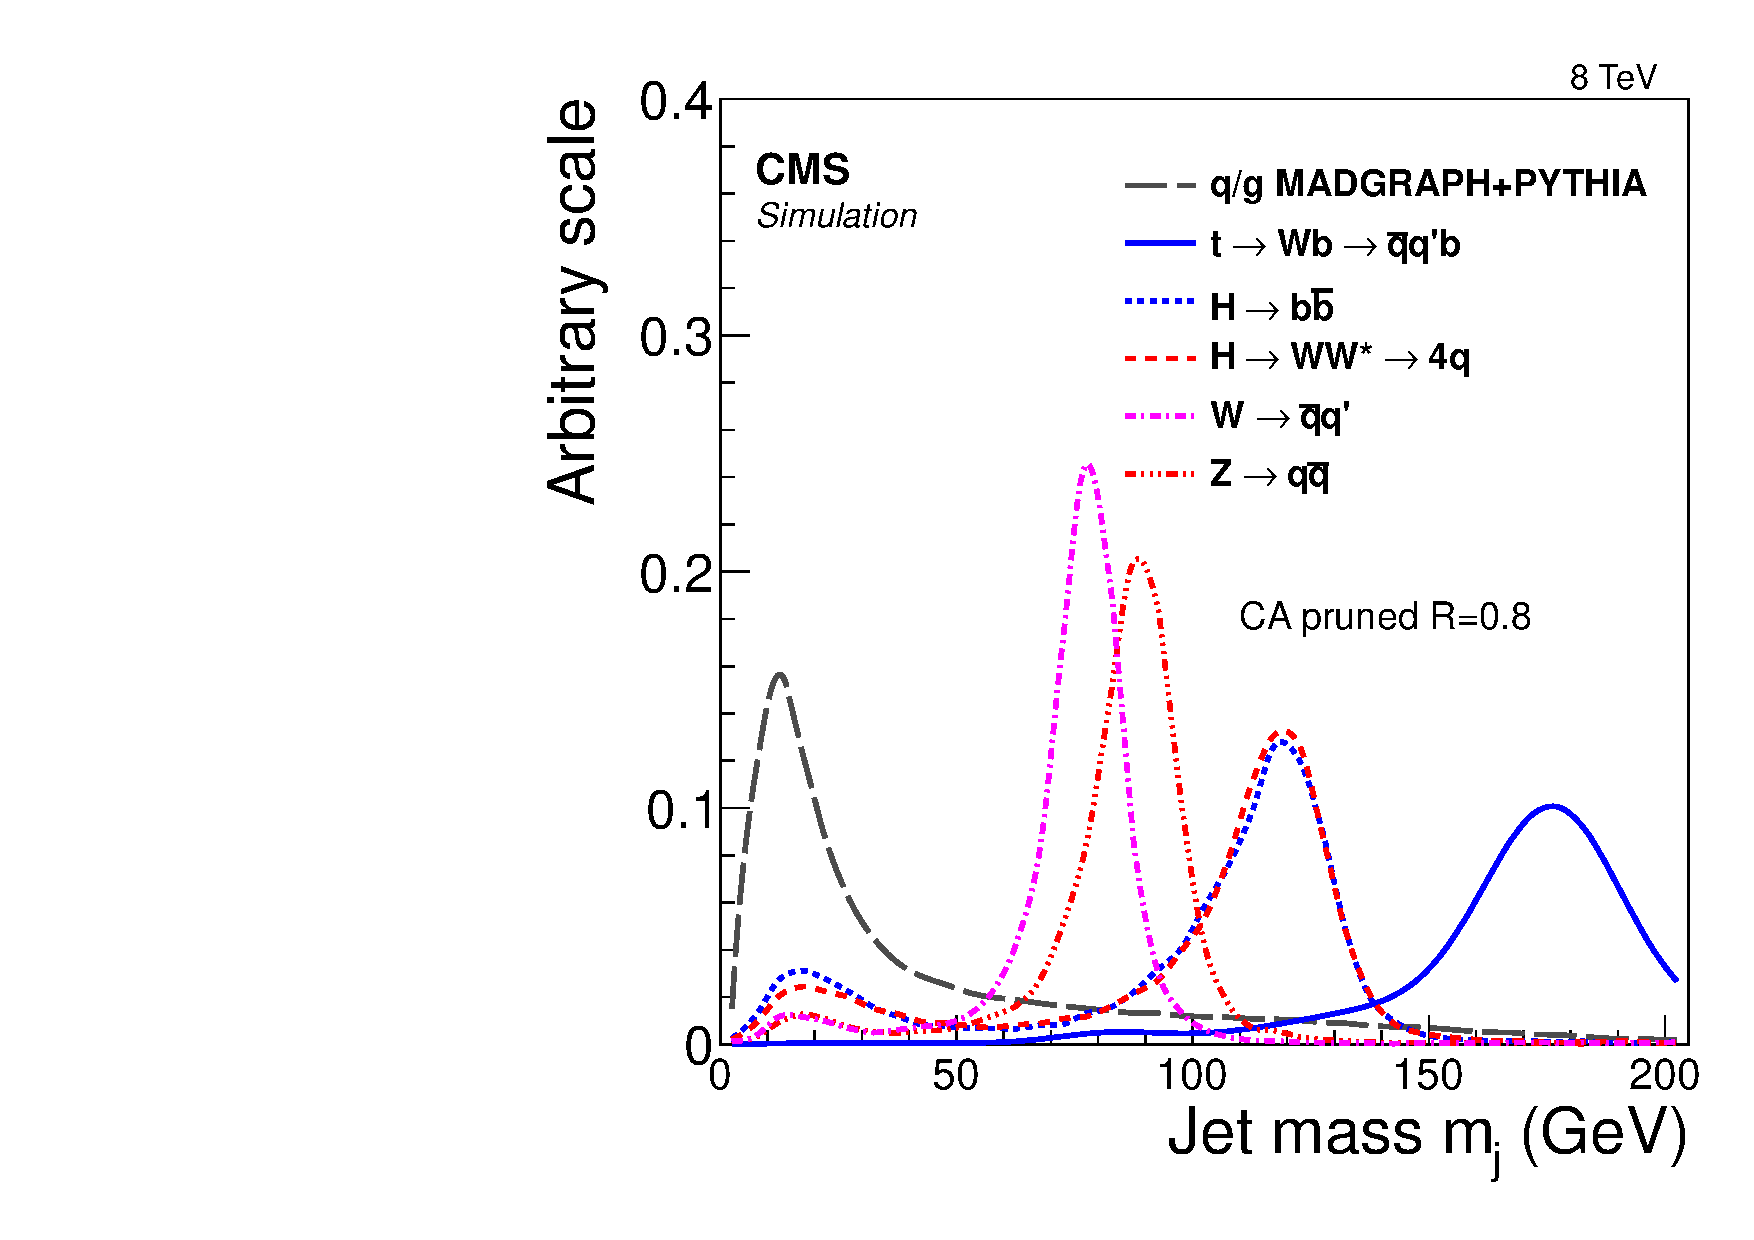
\includegraphics[width=0.69\textwidth]{HbbZqqfigs/Signal/signal-data-qcd-jetmass.pdf}
%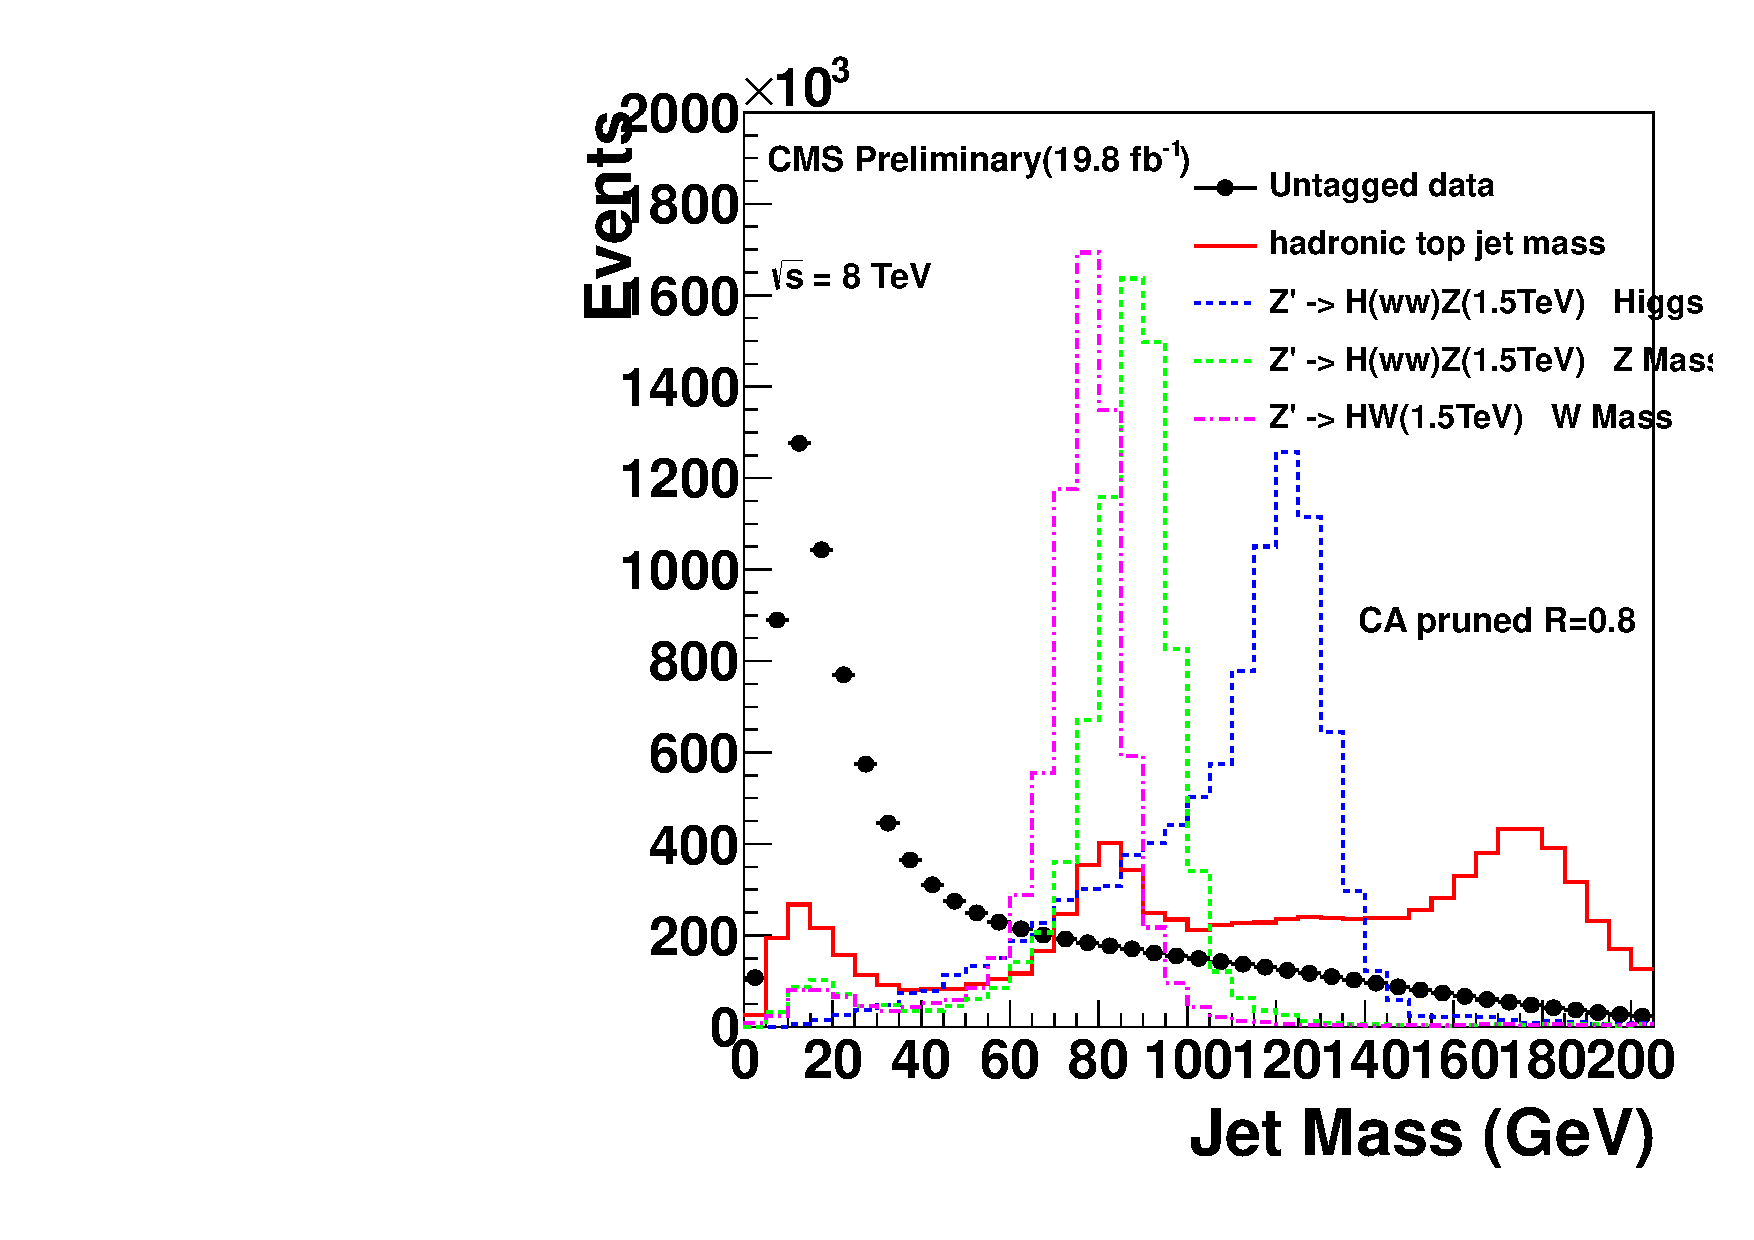
\includegraphics[width=0.49\textwidth]{HqqqqZqqfigs/Signal/signal-data-qcd-jetmass.pdf}
%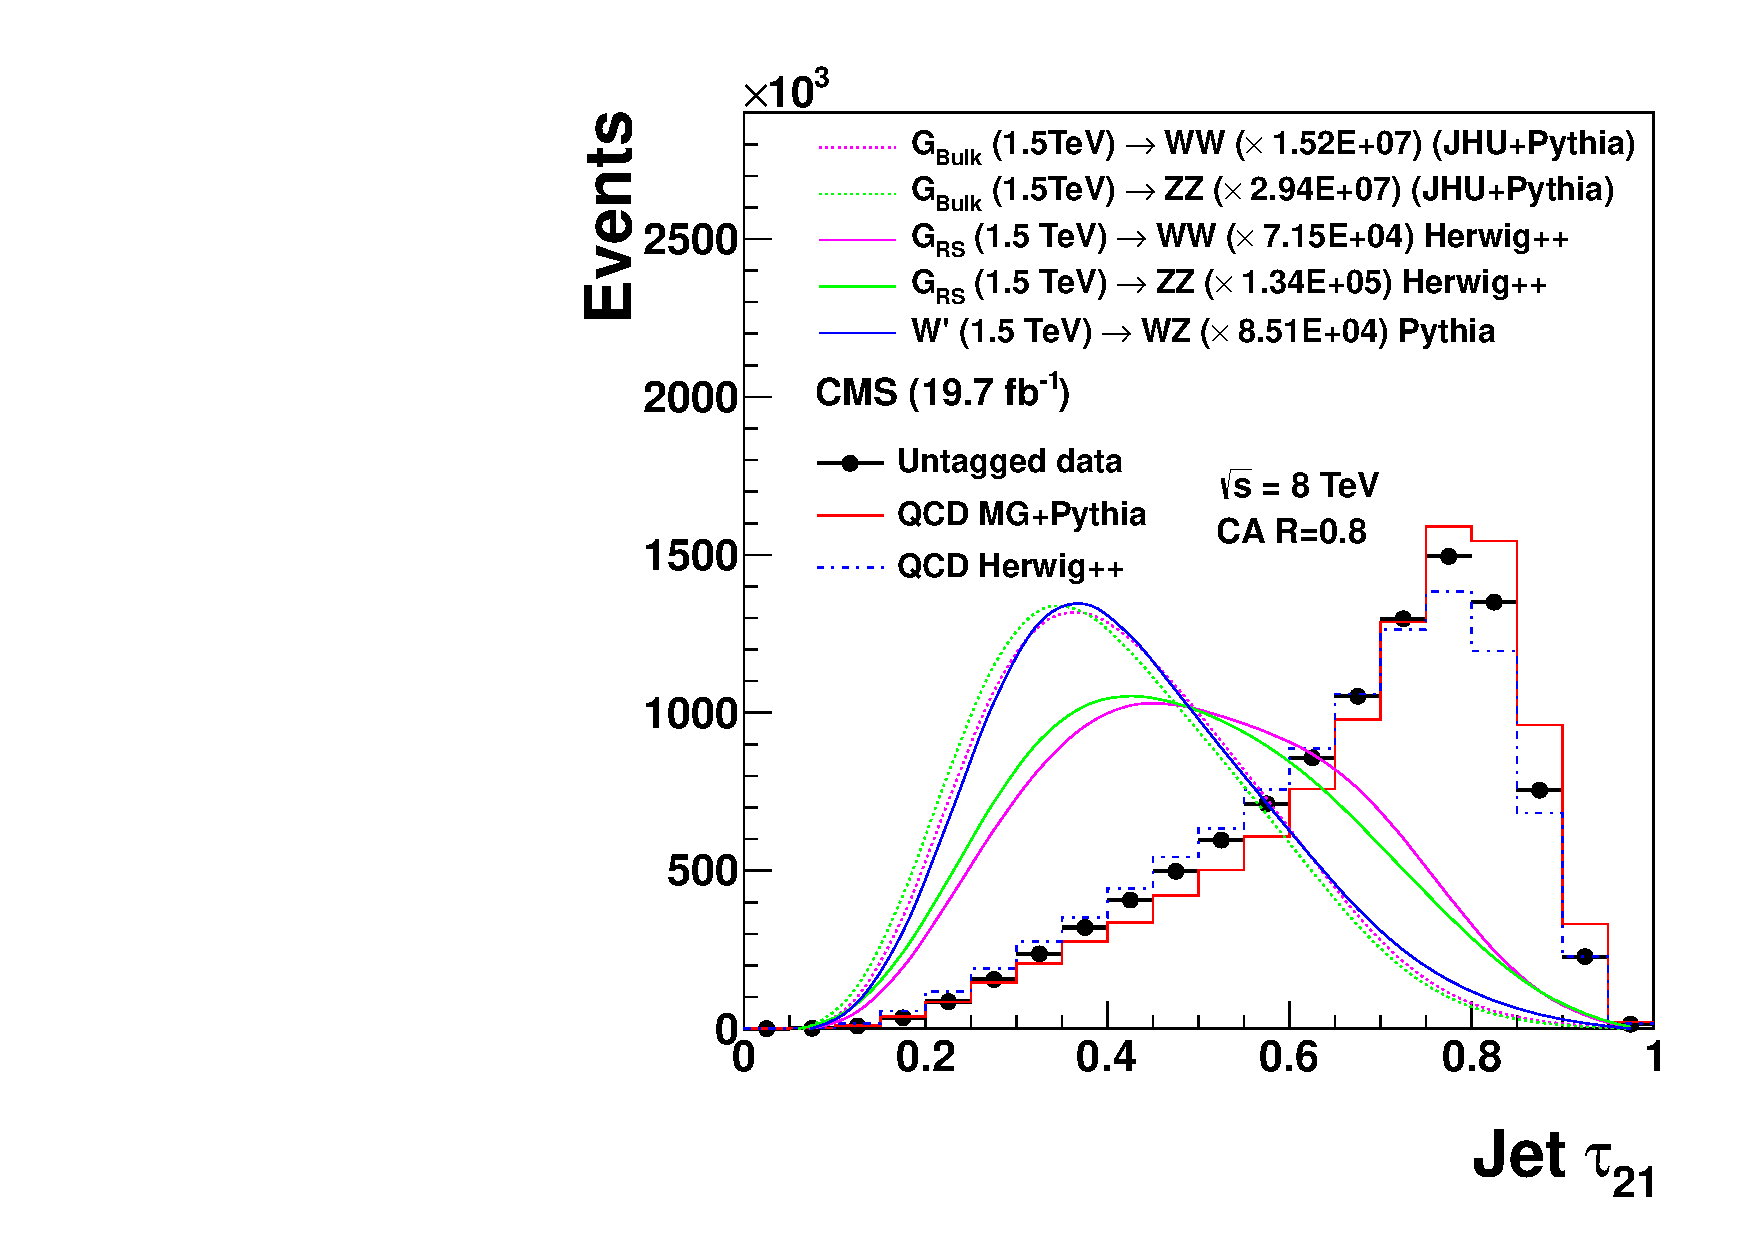
\includegraphics[width=0.49\textwidth]{figs/signal-acc-eff/signal-data-qcd-Jet-Tau21.pdf}
\end{center}
%\caption{Pruned jet mass in signal MC, data and background MC.
%All curves are plotted with the same binning.
%MC are randomly normalized to fit in the plot. H(bb) jets on the left plot, H(ww -> qqqq) on the right hand plot. 
%The signal MC distributions are plotted as smooth curves connecting the histogram entries. MC are normalized according to data.
%}
\caption{Pruned jet mass in signal MC, data and background MC.
All curves are plotted with the same binning.
MC are randomly normalized to fit in the plot. 
}
\label{fig:HbbjetMass}
\end{figure}

%Plot:  the pruned jet mass of Higgs Jet and QCD jet , Z jet, top jet? in one plot. 

%Plot:  tau42 for Higgs Jet , Z jets, WJets, top jet, in one plot. leptonic top jet ?


%The pruned jet mass and jet $\tau_{21}$ distributions in signal MC, data and background MC are shown in Fig.~\ref{fig:taggingvariables}.

Fully merged jets from Ws and Zs peak around 80-90~\GeV in pruned jet mass while QCD jets and not fully merged Ws and Zs peak around 20~\GeV.
Fully merged jets from Higgs to bb\bar decays peaked around 120~130\GeV. 
The discriminating power of the pruned jet mass for signals is evident.

and the tau42 distribution is already shown on the Htagging part. 

For both the pruned jet mass and $\tau_{42}$, differences are observed
between the \HERWIG{++} ($G_{RS}$) and \PYTHIA6
%($G_{Bulk}$, $\cPq^*$, $\PWpr$) distributions, which arise from
distributions, which arise from
differences in the polarization of the $\PW$/$\cPZ $ and Higgs bosons and the
showering and hadronization models used by these generators. 
The differences due to showering and hadronization models
are into account in the estimate of the systematic uncertainties

%In
%particular this is the reason why the $\PW\cPZ$ prediction for
%$\tau_{21}$ is different from the $\PW\PW$, $\cPZ\cPZ$ predictions.
%The differences due to showering and hadronization models
%%are into account in the estimate of the systematic uncertainties
%on the tagging efficiency, as discussed below.

%\begin{figure}[htb]
%\begin{center}
%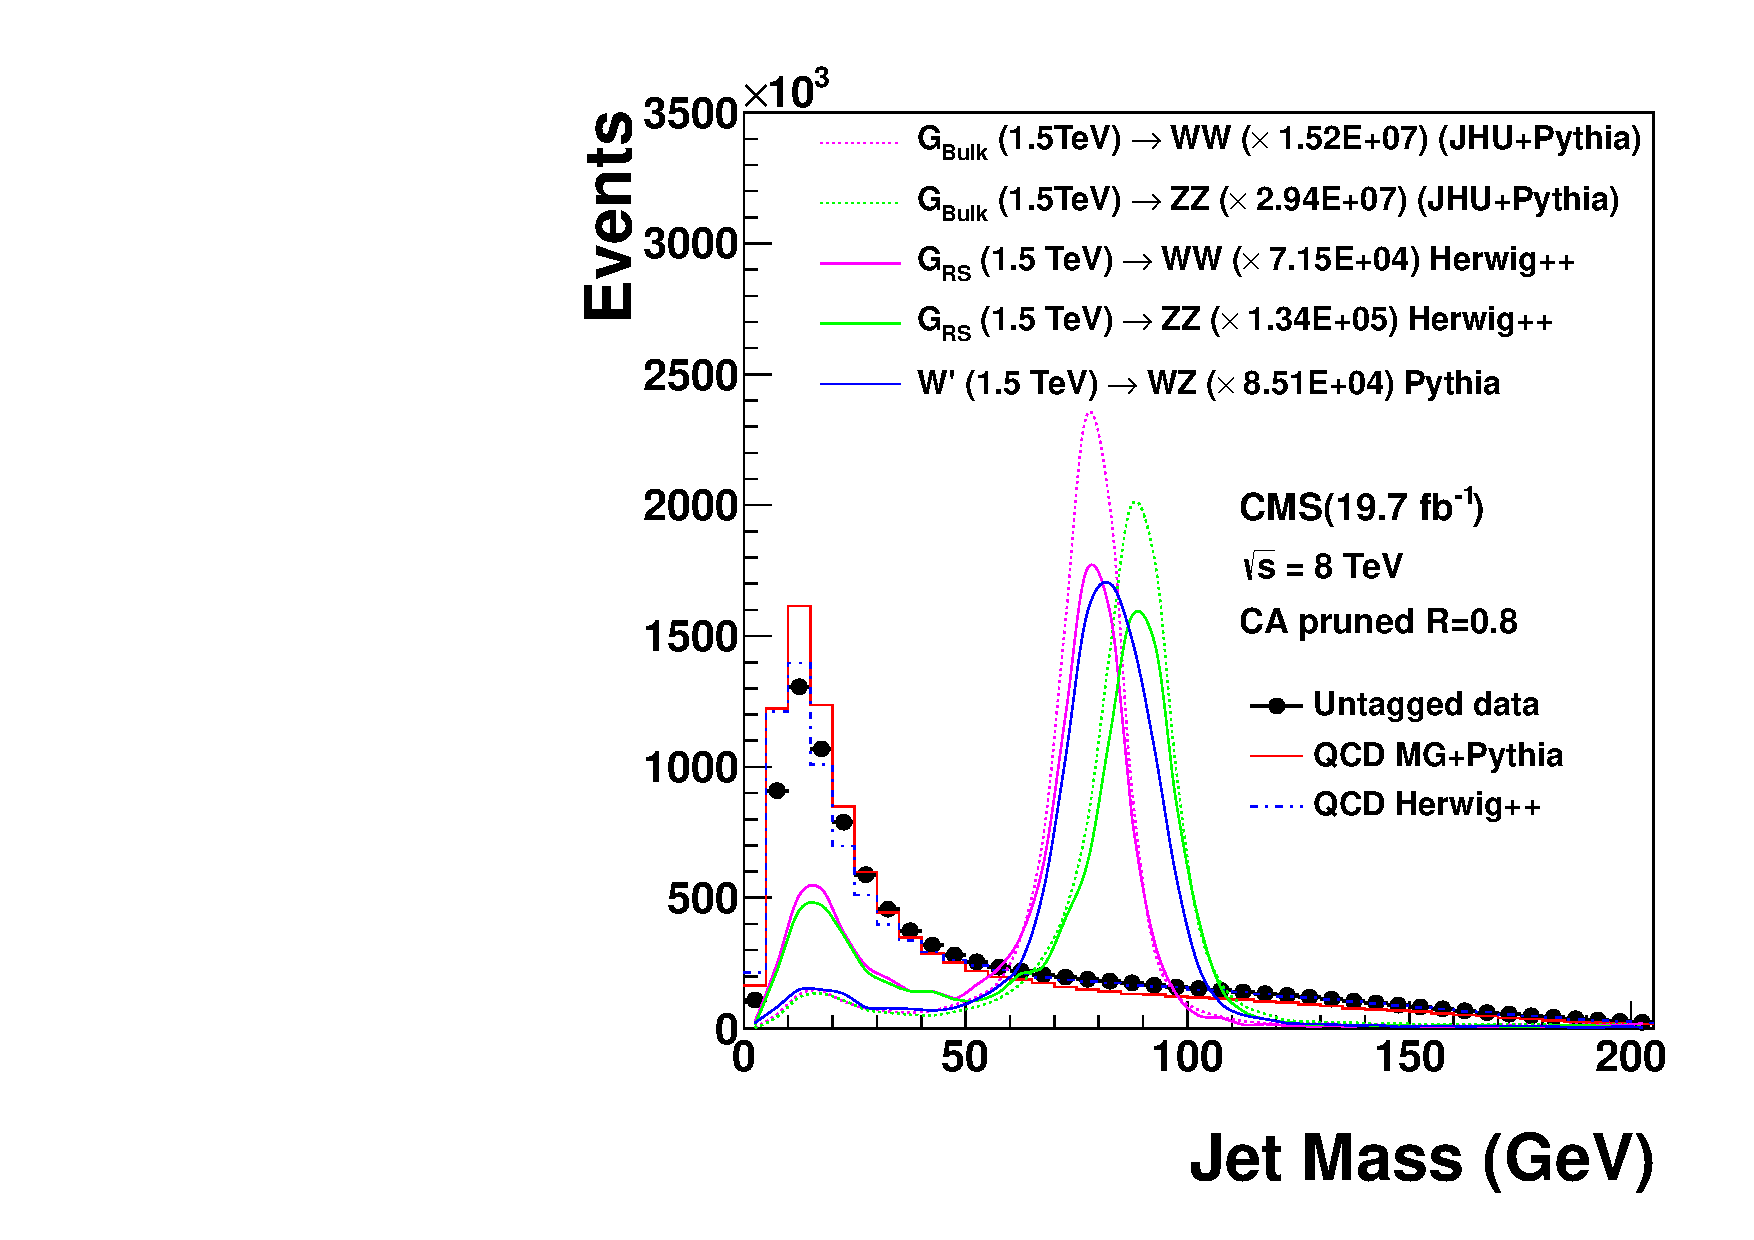
\includegraphics[width=0.49\textwidth]{figs/signal-acc-eff/signal-data-qcd-jetmass.pdf}
%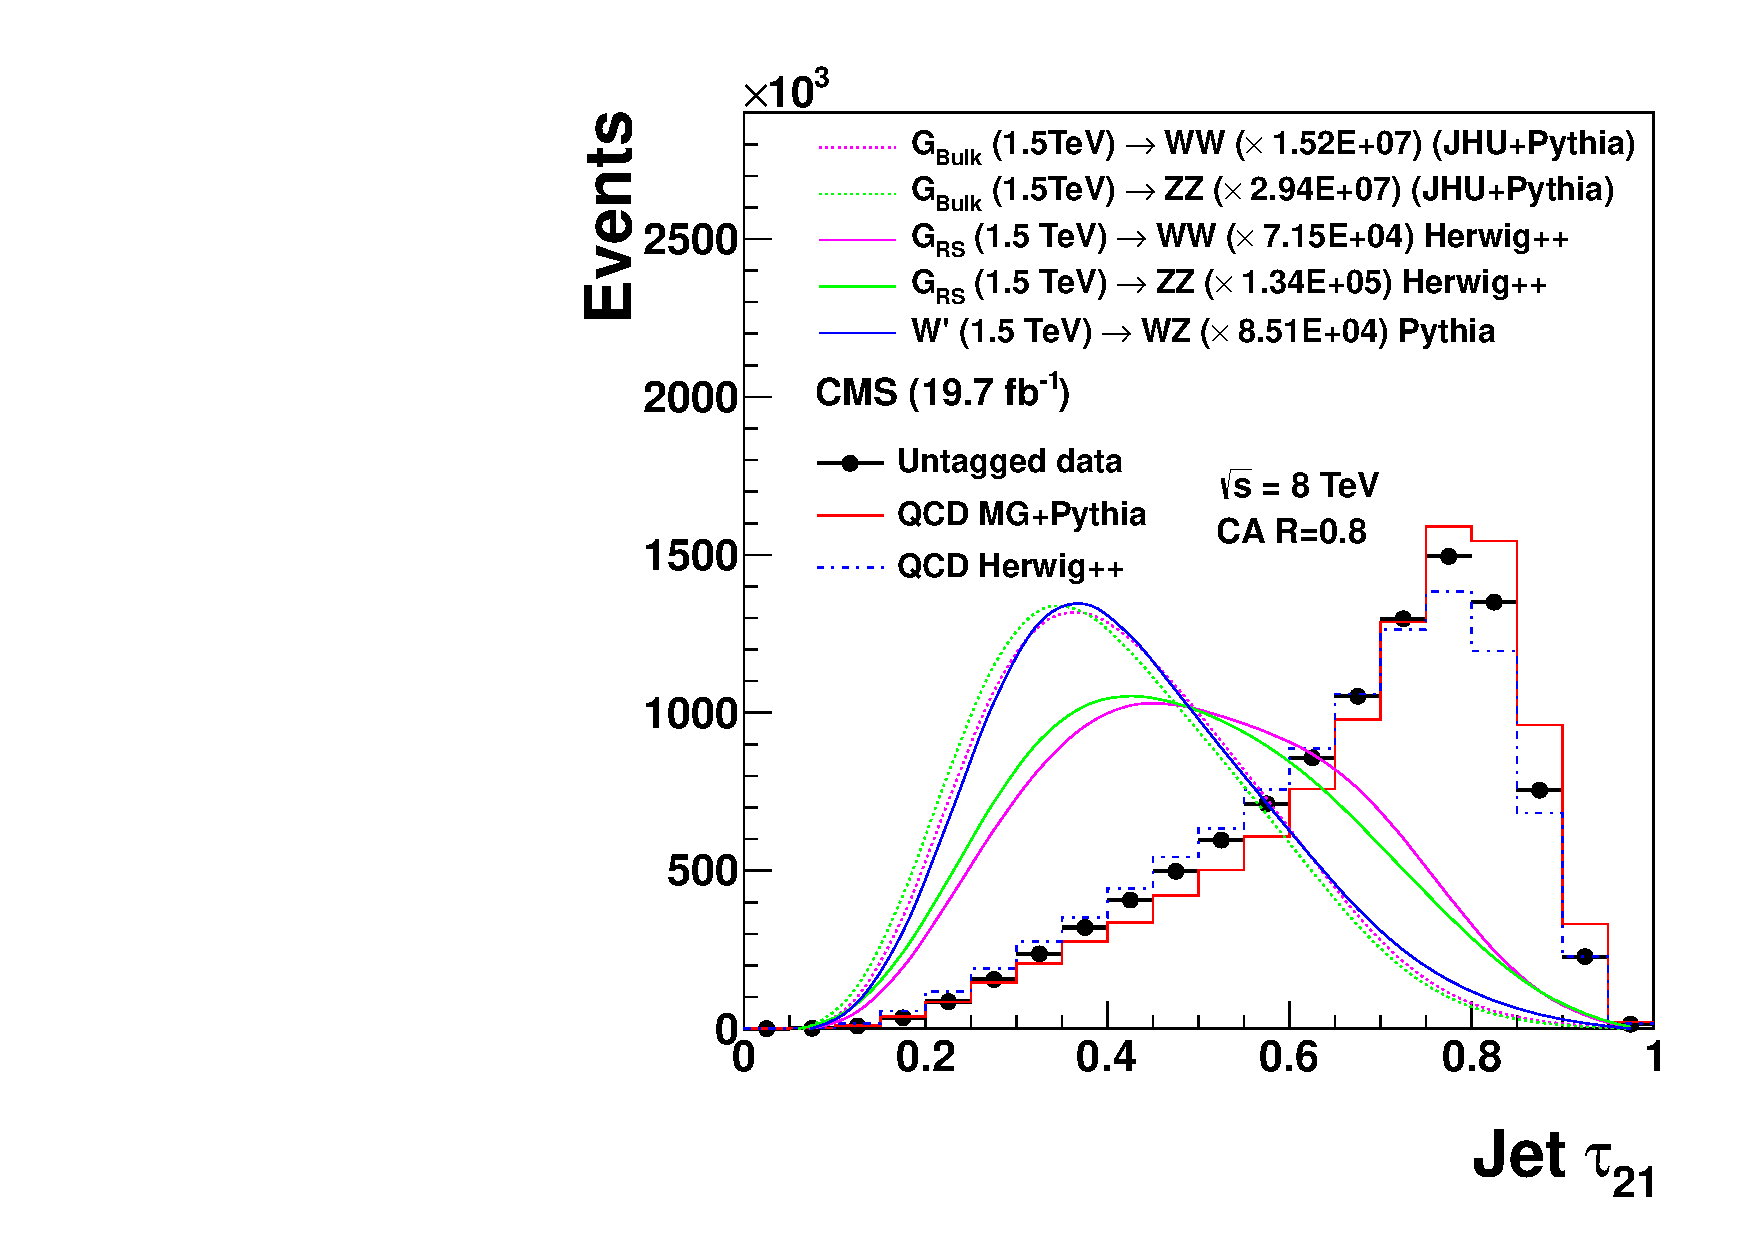
\includegraphics[width=0.49\textwidth]{figs/signal-acc-eff/signal-data-qcd-Jet-Tau21.pdf}
%\end{center}
%\caption{Pruned jet mass and $\tau_{21}$ in signal MC, data and background MC.
%All curves are plotted with the same binning.
%The signal MC distributions are plotted as smooth curves connecting the histogram entries. MC are normalized according to data.
%}
%\label{fig:taggingvariables}
%\end{figure}

%Table~\ref{table:acceptance} summarizes the signal branching ratio times angular acceptances and also the W/Z-tagging efficiencies.

%The Higgs tagging efficiency 

We study the Higgs tagging efficiency in MC by matching the jet to the Higgs Gen particle, 
this is jet is refered as Higgs genJet. 
And then apply the H-tagging rule on the Higgs genJet.
Fig.~\ref{fig:HEff} are showing the Higgs tagging efficiency 
of H(bb) and H(ww) jets. 


\begin{figure}[htb]
\begin{center}
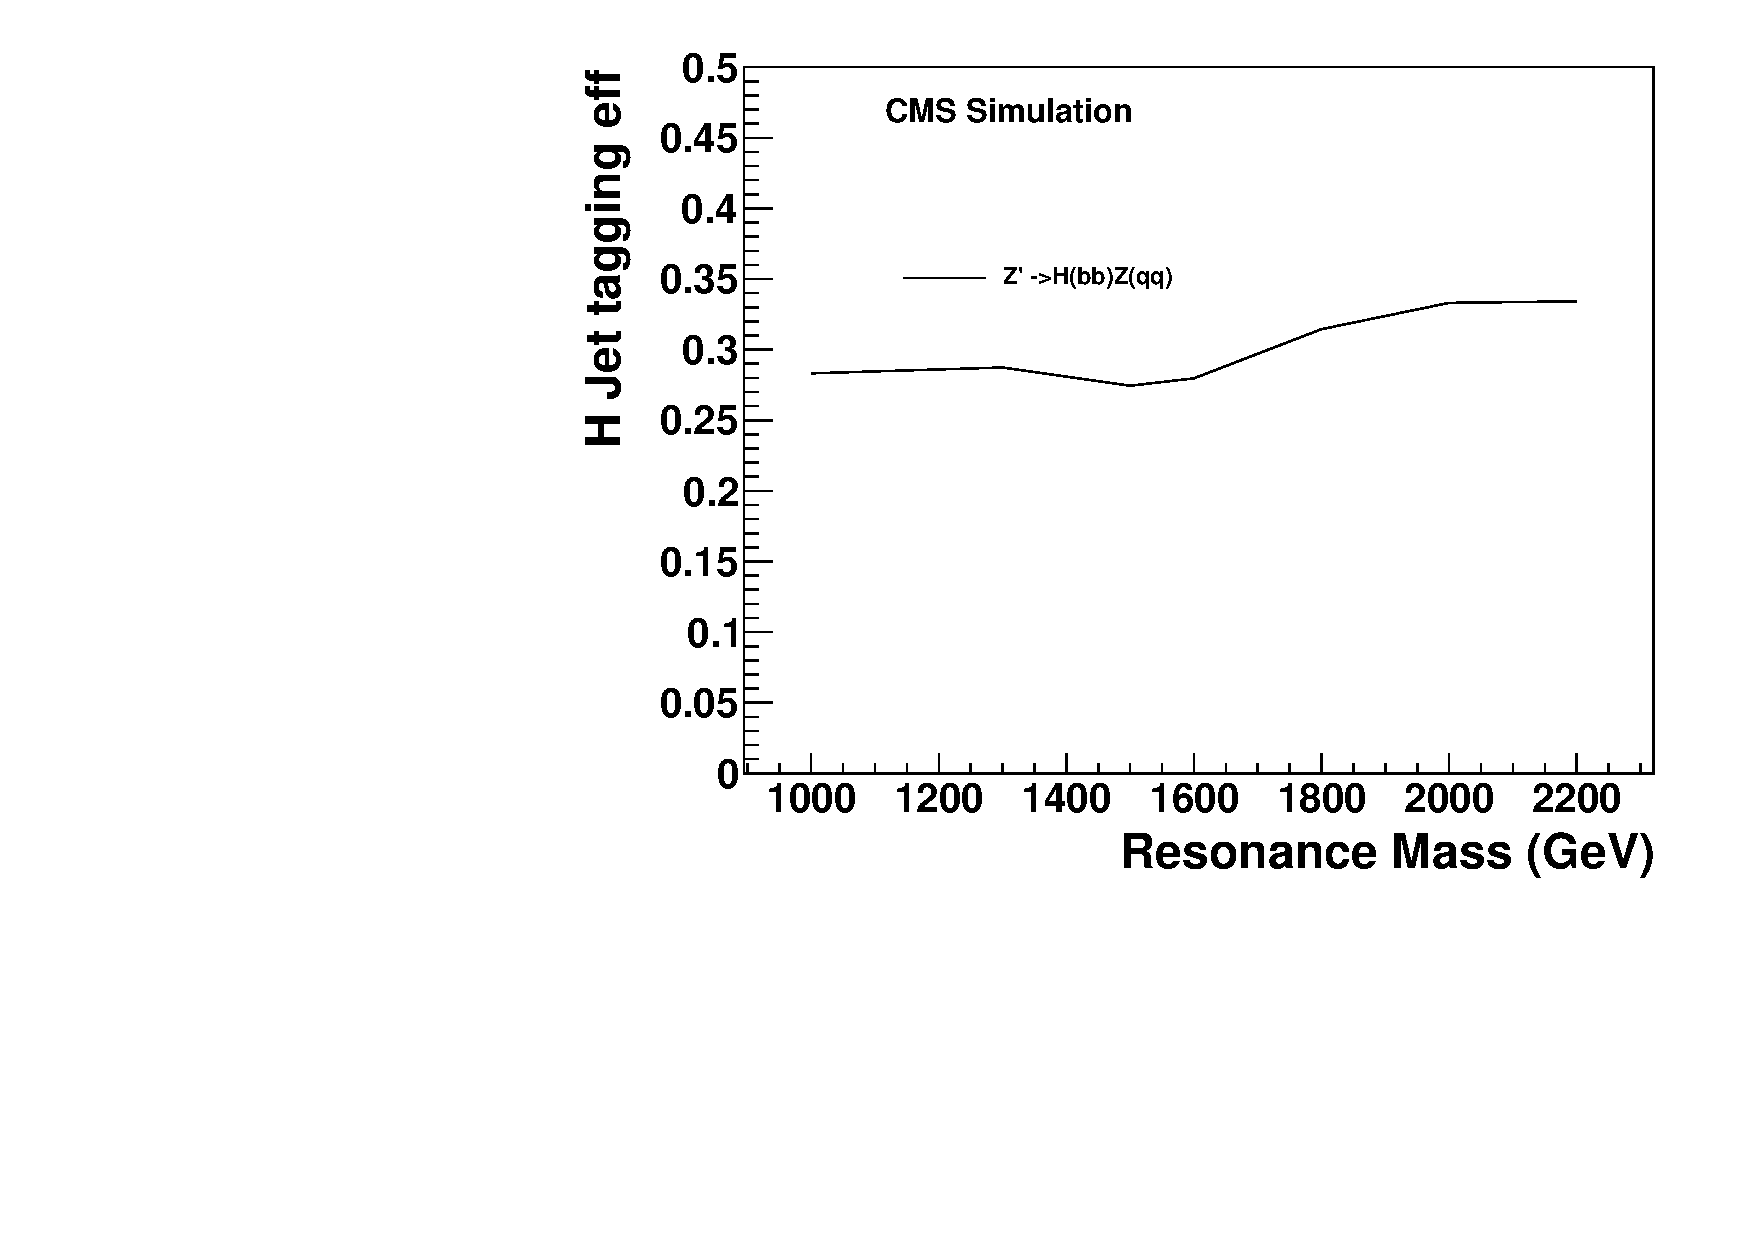
\includegraphics[width=0.49\textwidth]{HbbZqqfigs/Signal/H-taggingEff-8TeV.pdf}
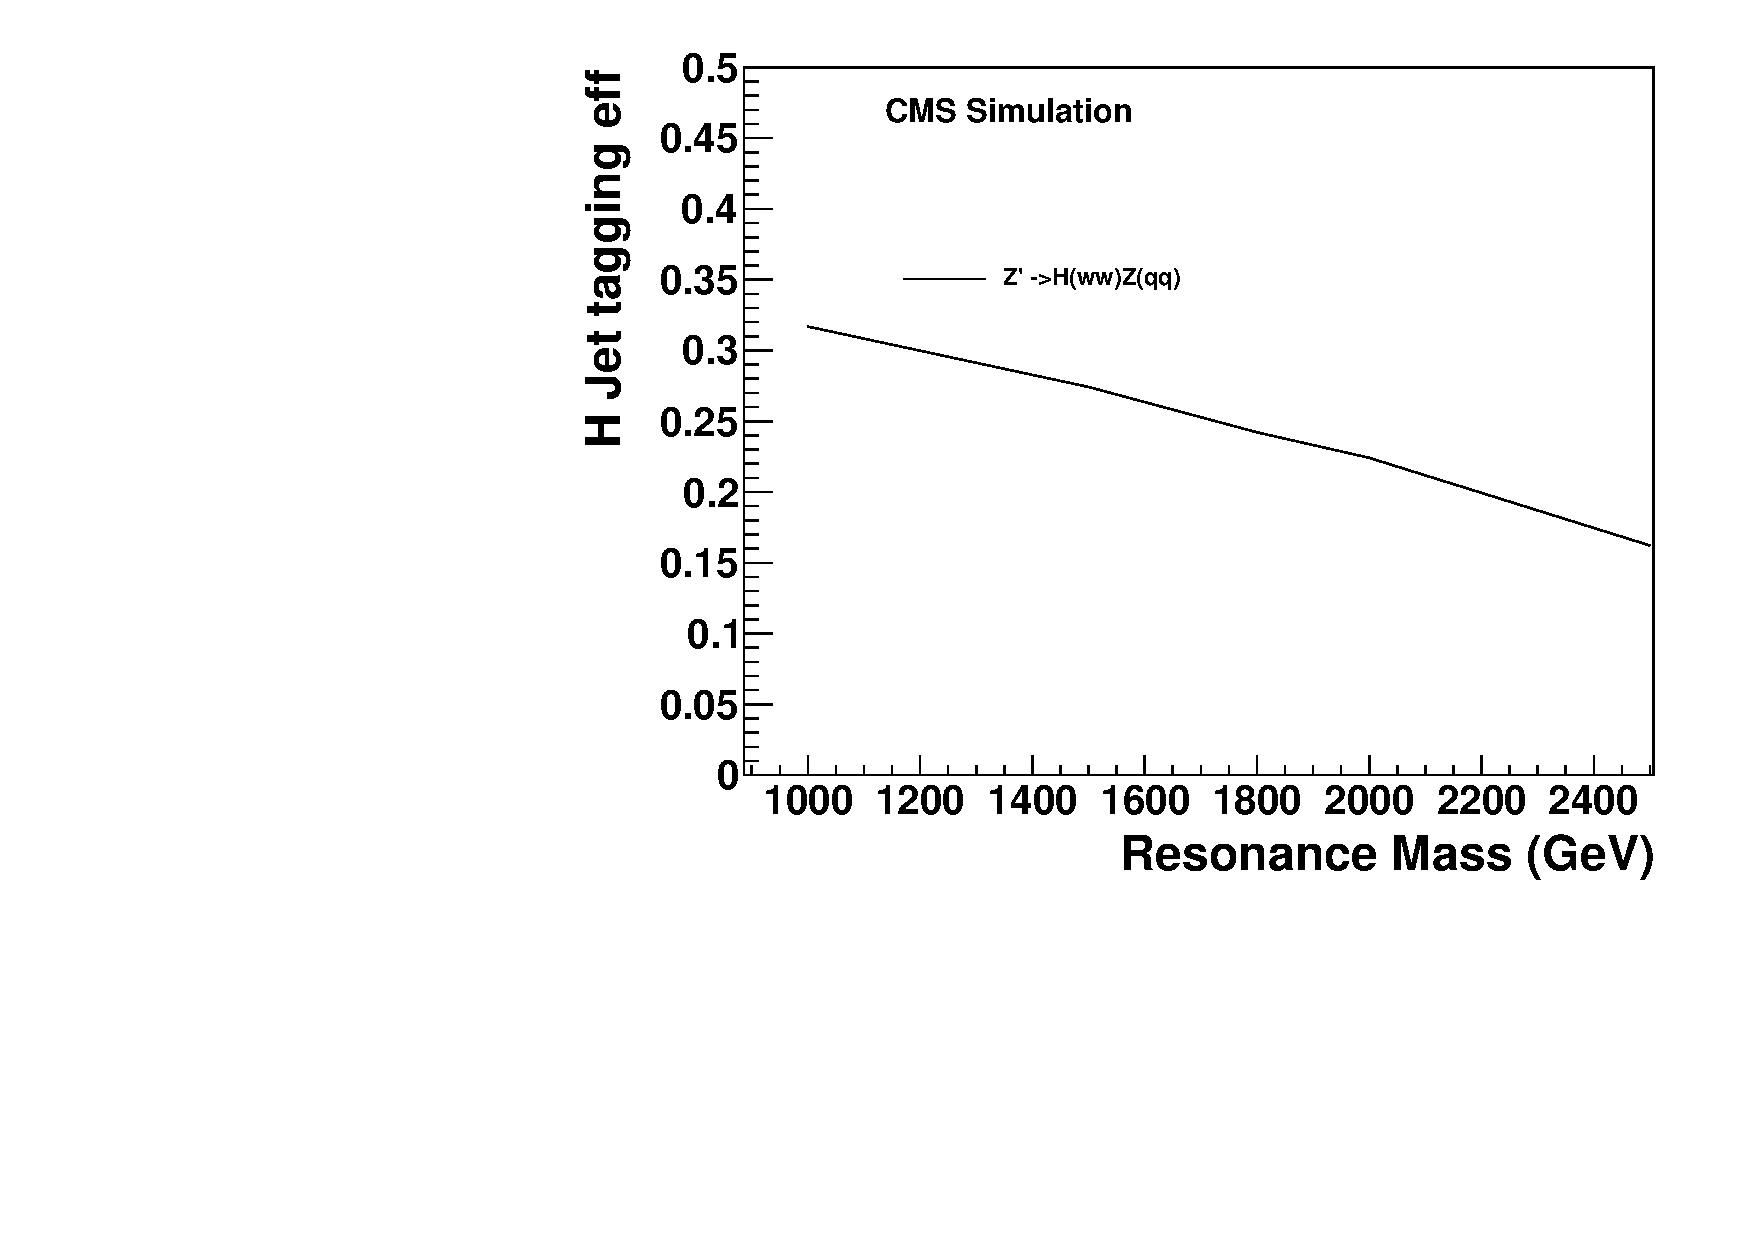
\includegraphics[width=0.49\textwidth]{HqqqqZqqfigs/Signal/H-taggingEff-8TeV.pdf}
%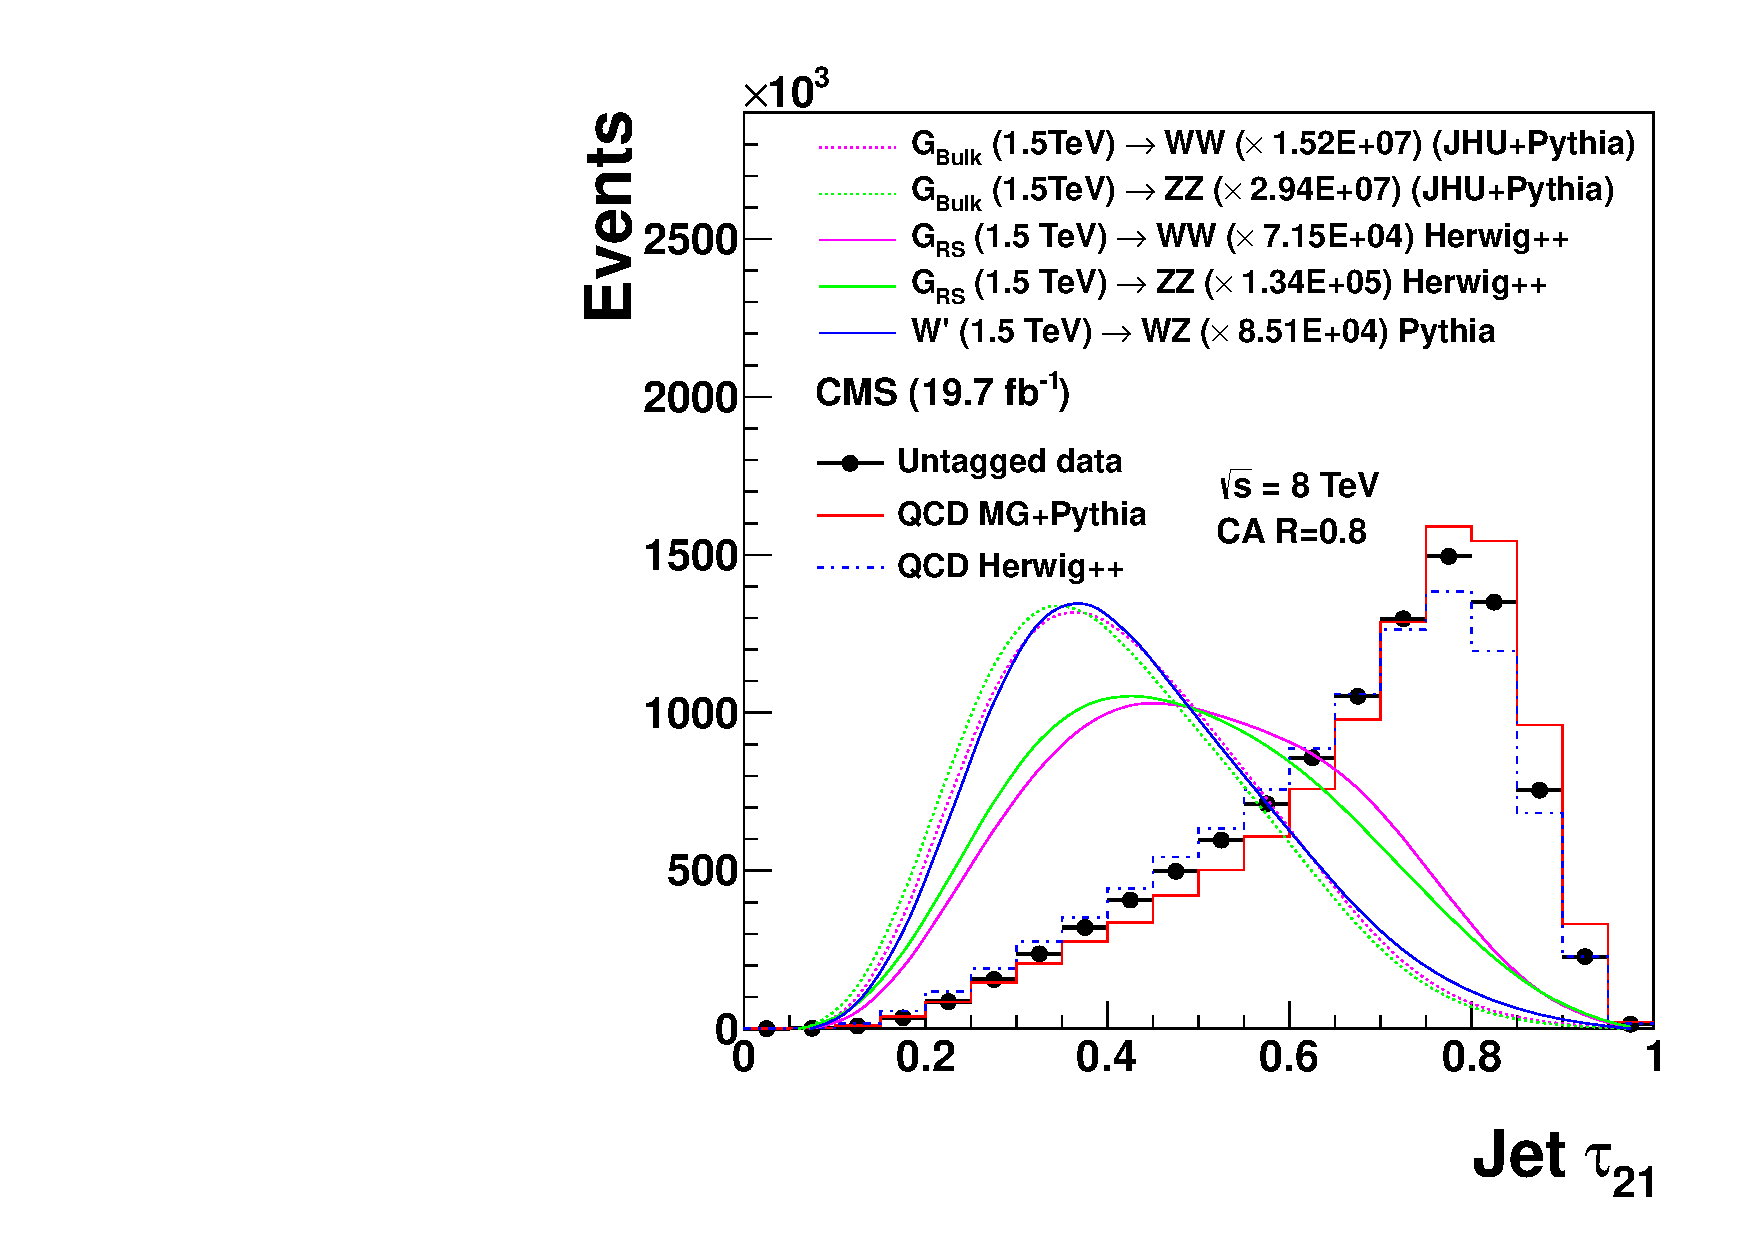
\includegraphics[width=0.49\textwidth]{figs/signal-acc-eff/signal-data-qcd-Jet-Tau21.pdf}
\end{center}
\caption{
Higgs genJet tagging efficiency in signal mc.On the left is H(bb), on the right hand is H(ww).  
}
\label{fig:HEff}
\end{figure}

In the Hbb channel, we see the upward movment of Hbb tagging efficiency. At high resonance, above 1.5 \TeVc
for signal,  H jets will be boosted to have deltaR smaller than 0.3. And the fat jet b tagging will be applied. 
So we may change fat jet b tagging to CSVM, which will introduce a smooth falling H-tagging eff, as shown in 
Fig.~\ref{fig:fatCSVM}. 


\begin{figure}[htb]
\begin{center}
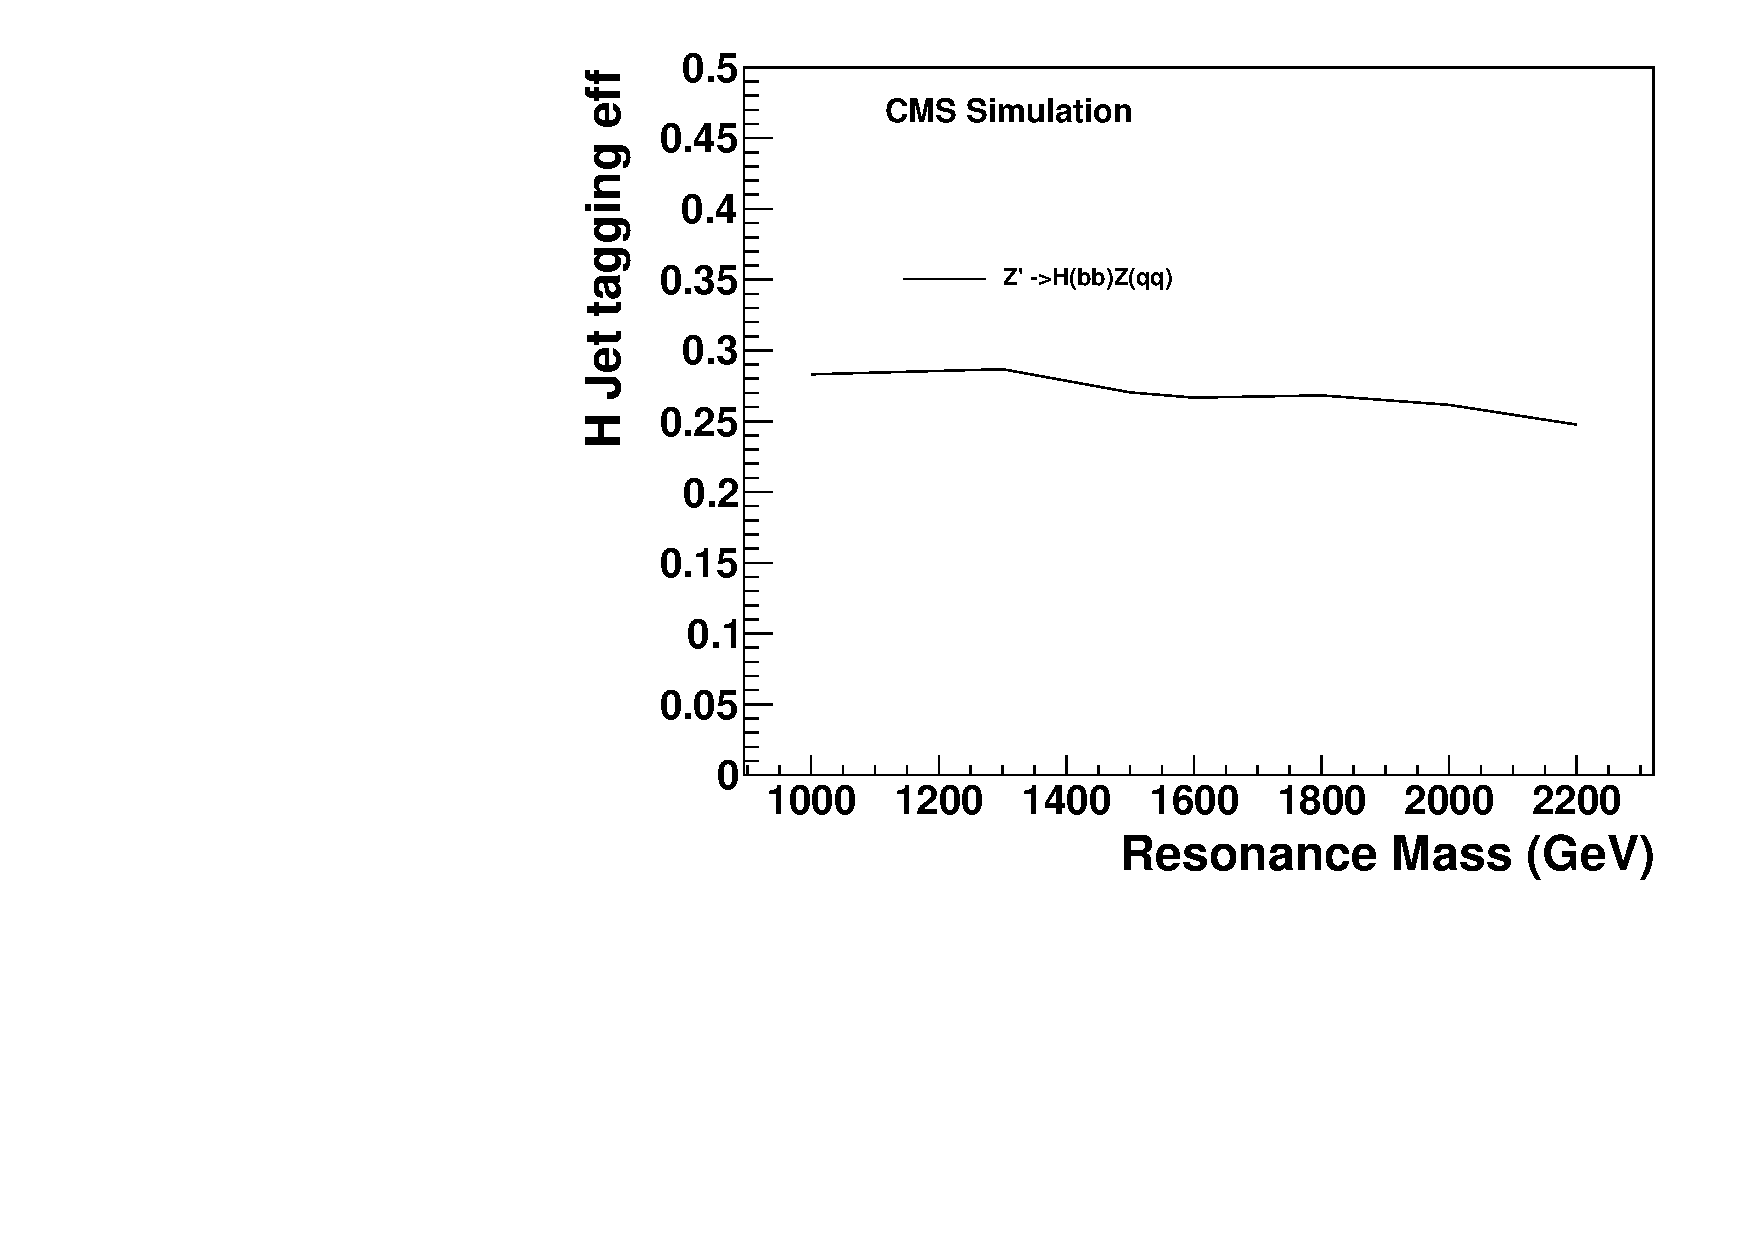
\includegraphics[width=0.60\textwidth]{HbbZqqfigs/Signal/H-taggingEff-8TeV-CSVM.pdf}
\end{center}
\caption{
Higgs genJet tagging efficiency in signal mc, for H(bb) channel.  Changing fat jet b tagging to CSVM instead of CSVL. 
}
\label{fig:fatCSVM}
\end{figure}


In the H(ww) all hadronic channel, to compensate the efficiency drop in the high resonance mass, we also add two low purity 
categories, low purity H-tagging and low purity V-tagging. 
The tagging efficiency of low purity H/V-tagging is shown on Fig.~\ref{fig:LowPurity}.  

\begin{figure}[htb]
\begin{center}
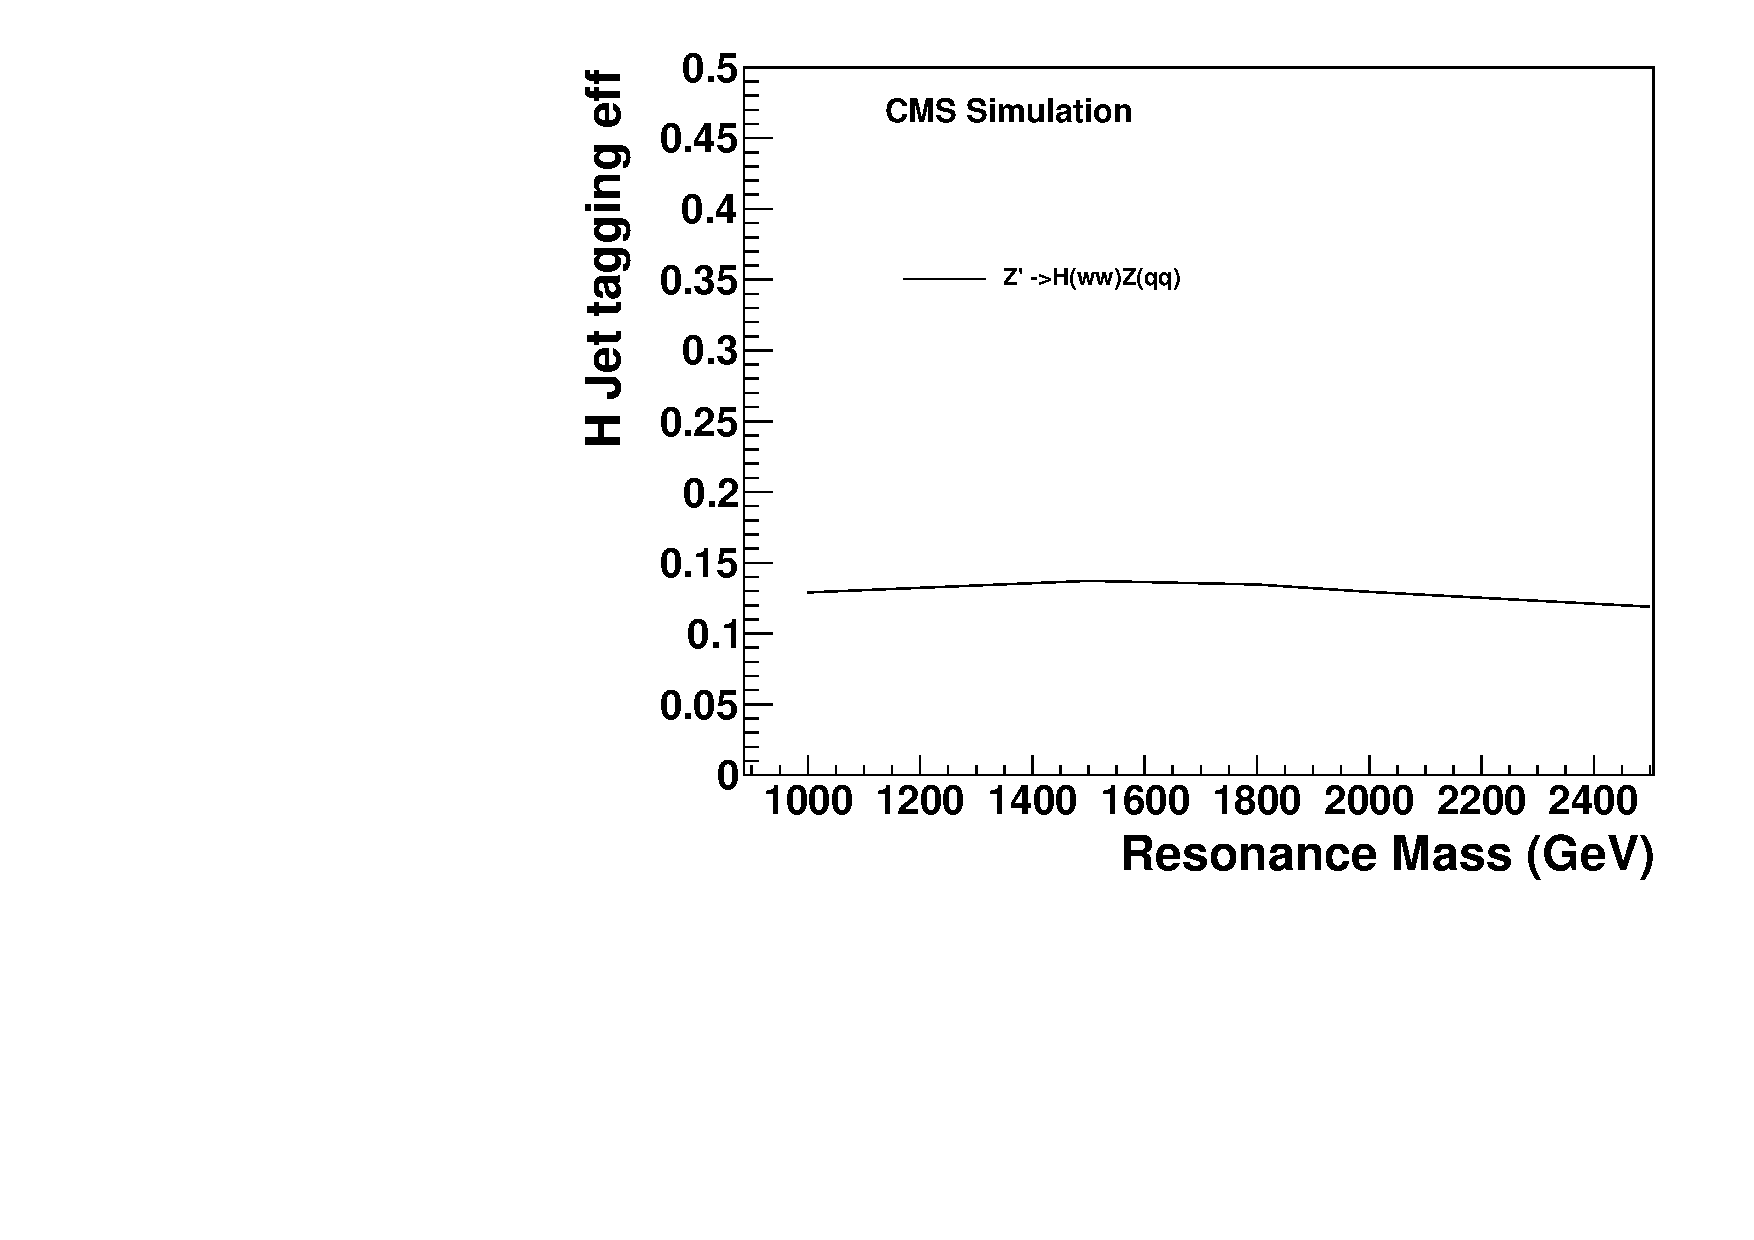
\includegraphics[width=0.49\textwidth]{HqqqqZqqfigs/Signal/H-taggingEff-8TeV-LowP.pdf}
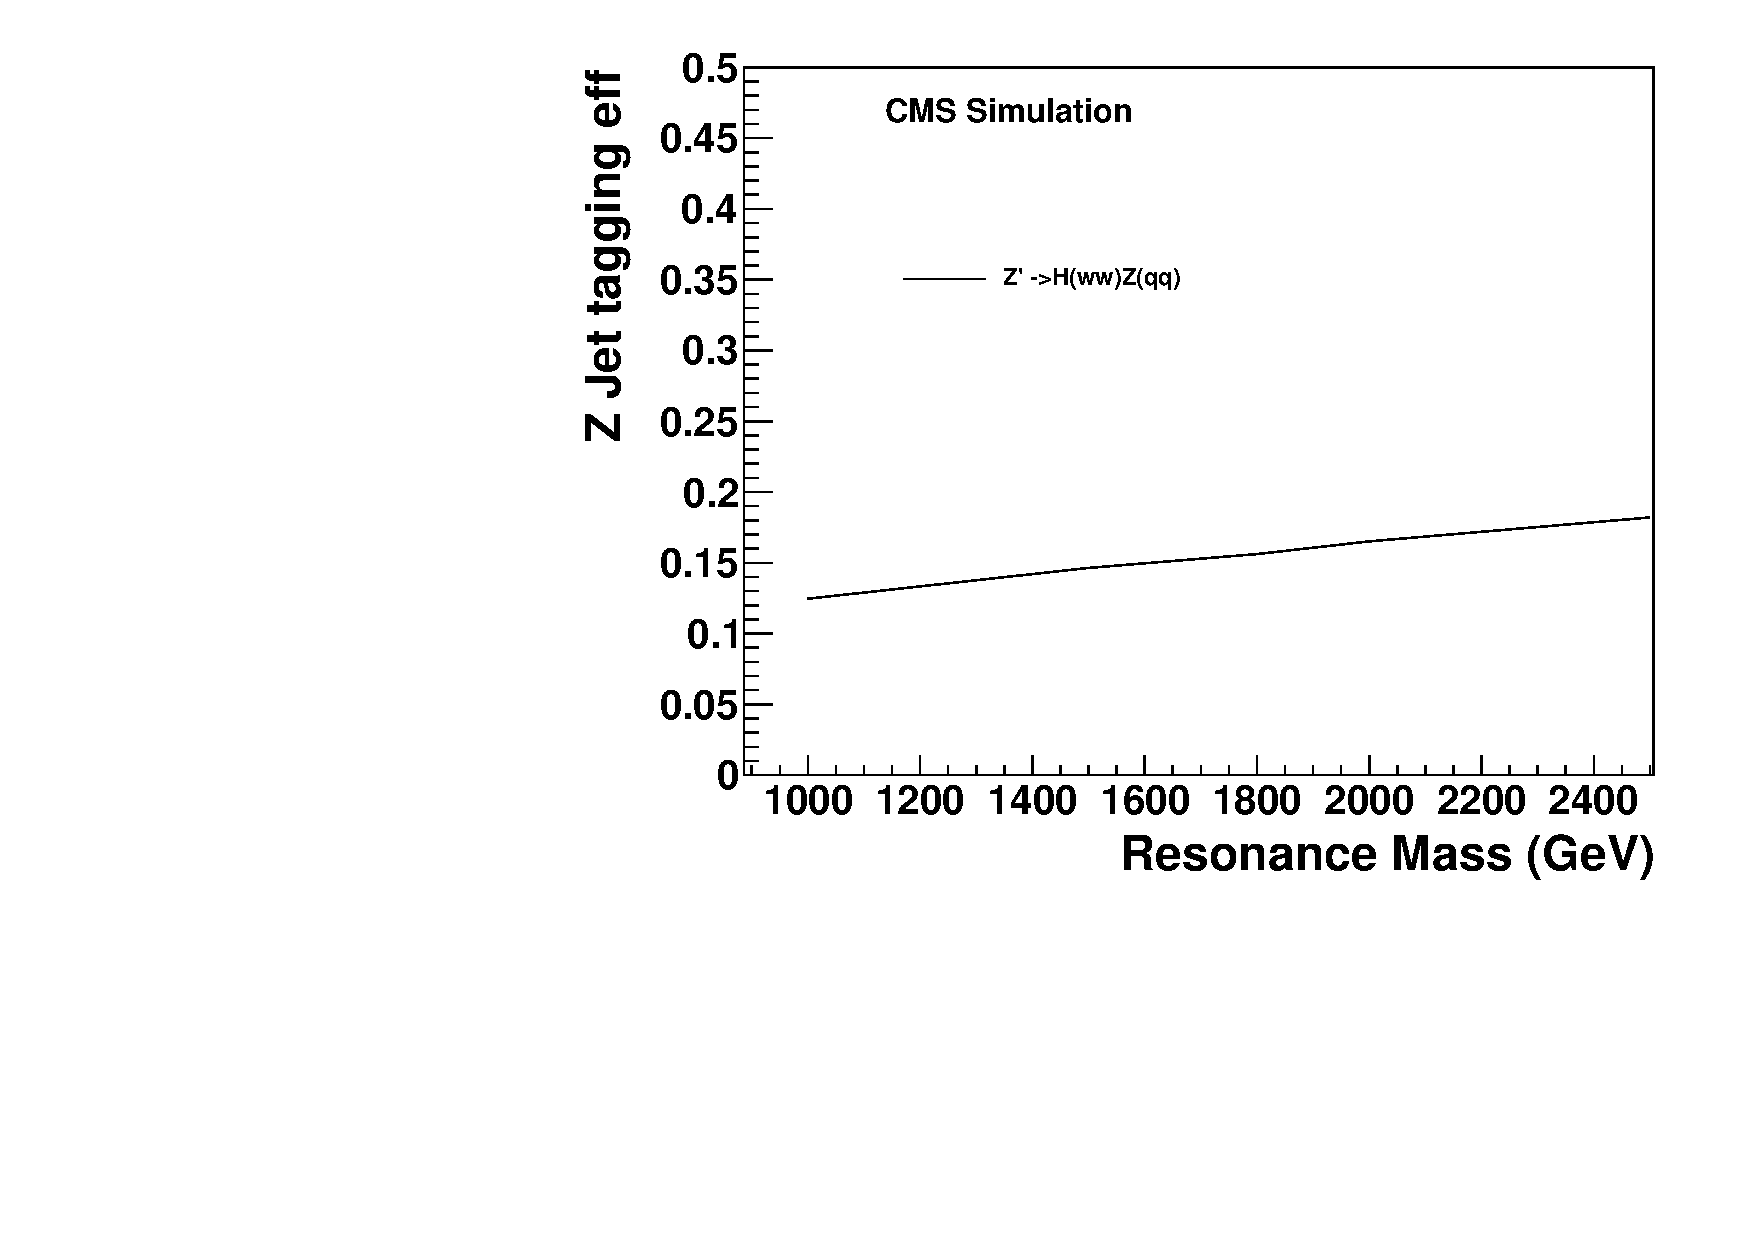
\includegraphics[width=0.49\textwidth]{HqqqqZqqfigs/Signal/Z-taggingEff-8TeV-LowP.pdf}
\end{center}
\caption{
Higgs genJet tagging efficiencies in signal mc, H(ww) low purity on left. Z(qq) low purity on right.  
}
\label{fig:LowPurity}
\end{figure}

{\bf  ACCEPTANCE}

Signal acceptance is defined as the number of signal events pass all the events selection divided by the 
number of generated events, shown on Fig.~\ref{fig:Acc}

\begin{figure}[htb]
\begin{center}
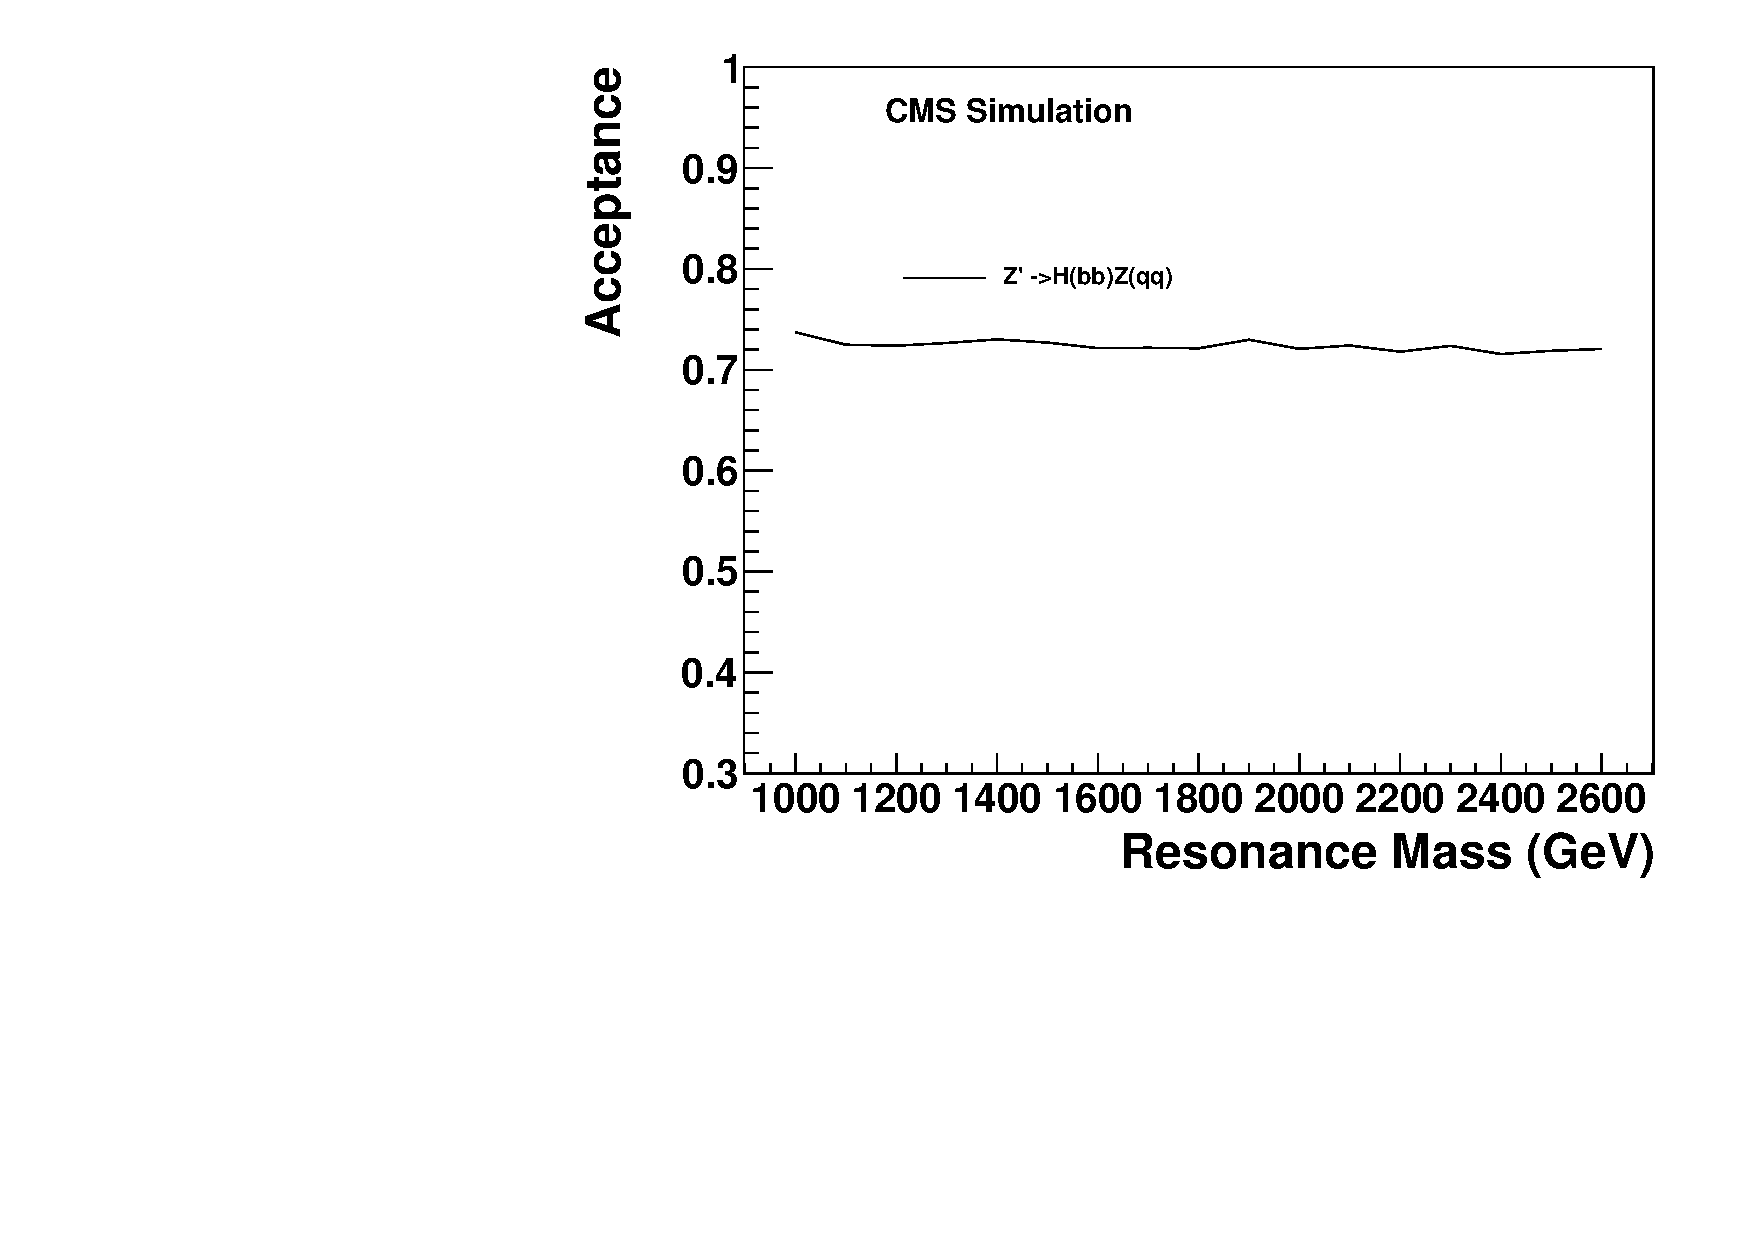
\includegraphics[width=0.49\textwidth]{HbbZqqfigs/Signal/HbbZqq-signal-acc-8TeV.pdf}
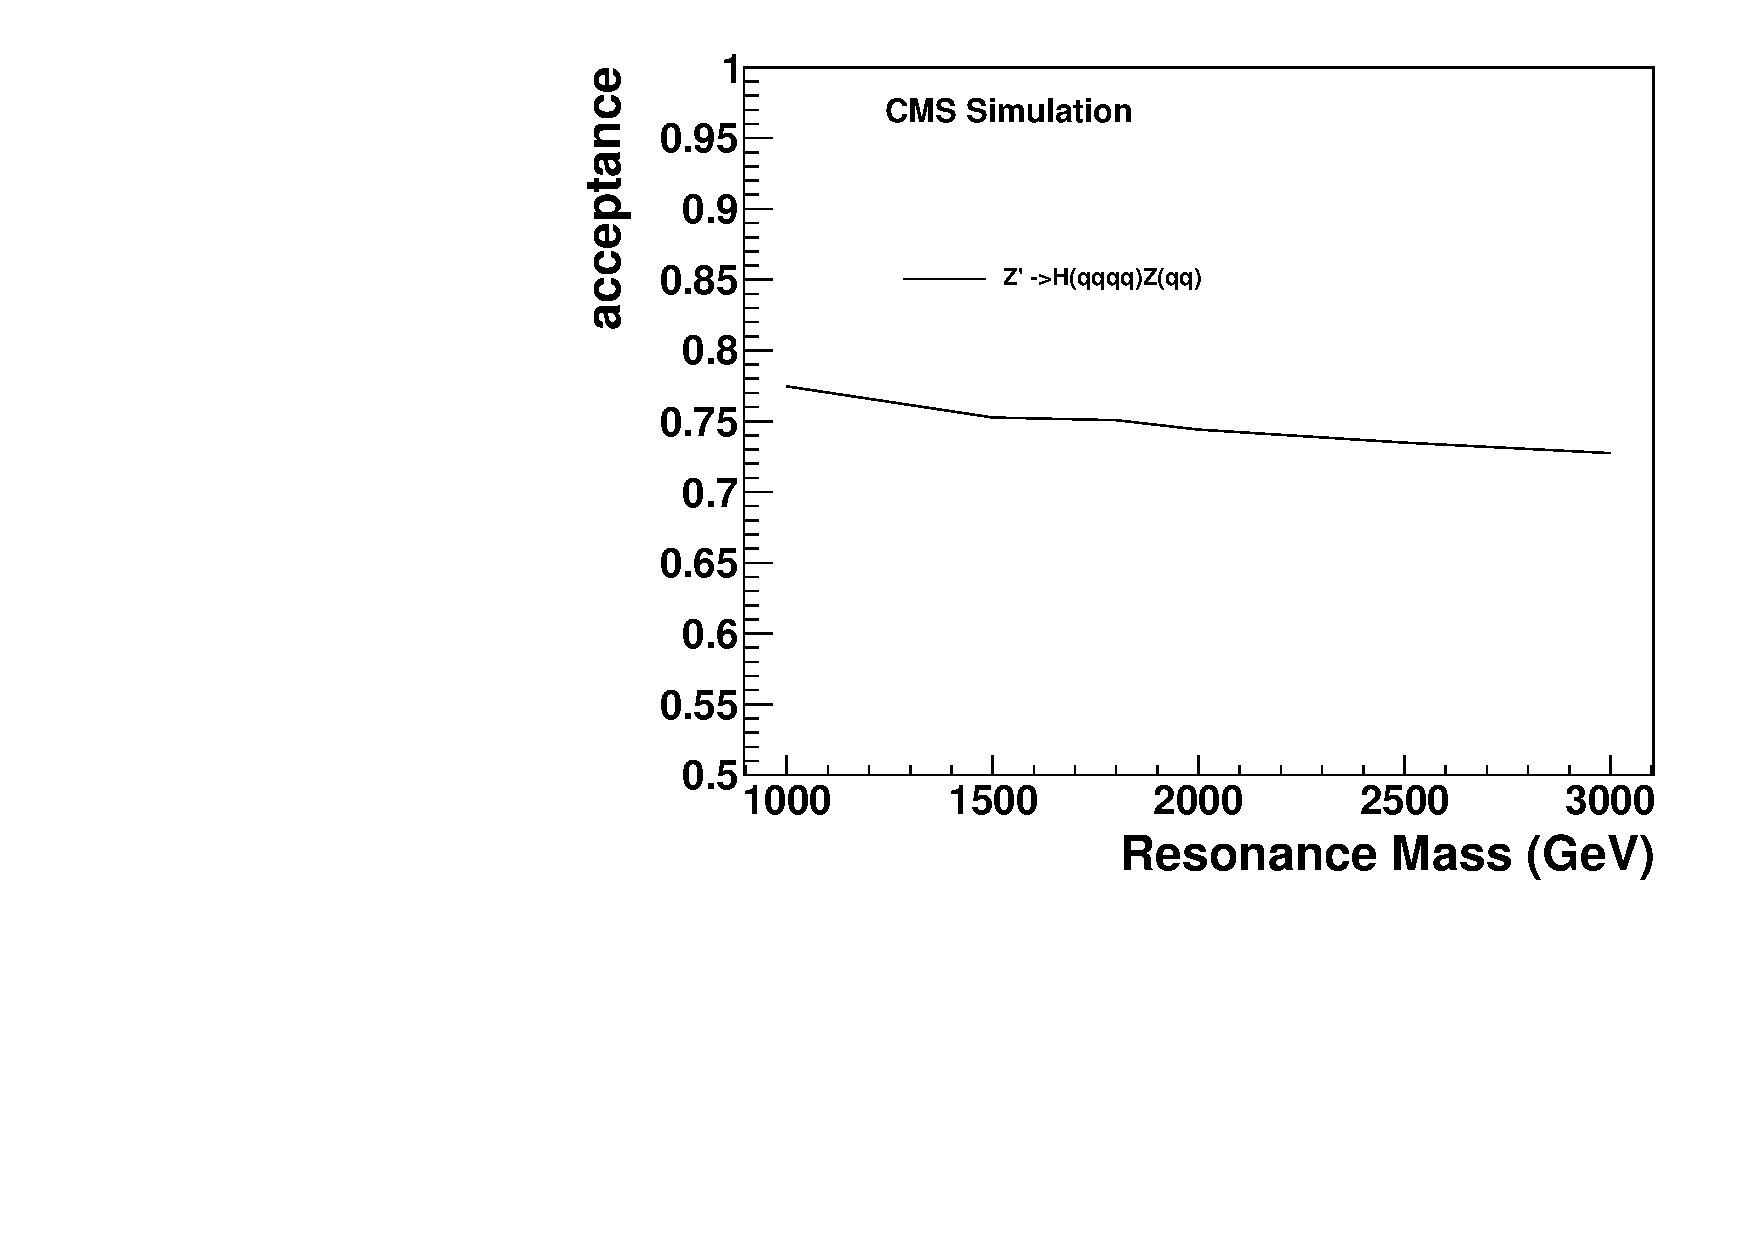
\includegraphics[width=0.49\textwidth]{HqqqqZqqfigs/Signal/HqqqqZqq-signal-acc-8TeV.pdf}
\end{center}
\caption{
Acceptance in signal. Left hand is H(bb), right hand is H(ww).
}
\label{fig:Acc}
\end{figure}


The overall tagging eff of Hbb channel in signal and data are shown on Fig.~\ref{fig:HbbEff}
and the tagging eff of H(ww) channel are shown on Fig.~\ref{fig:HwwEff}


\begin{figure}[htb]
\begin{center}
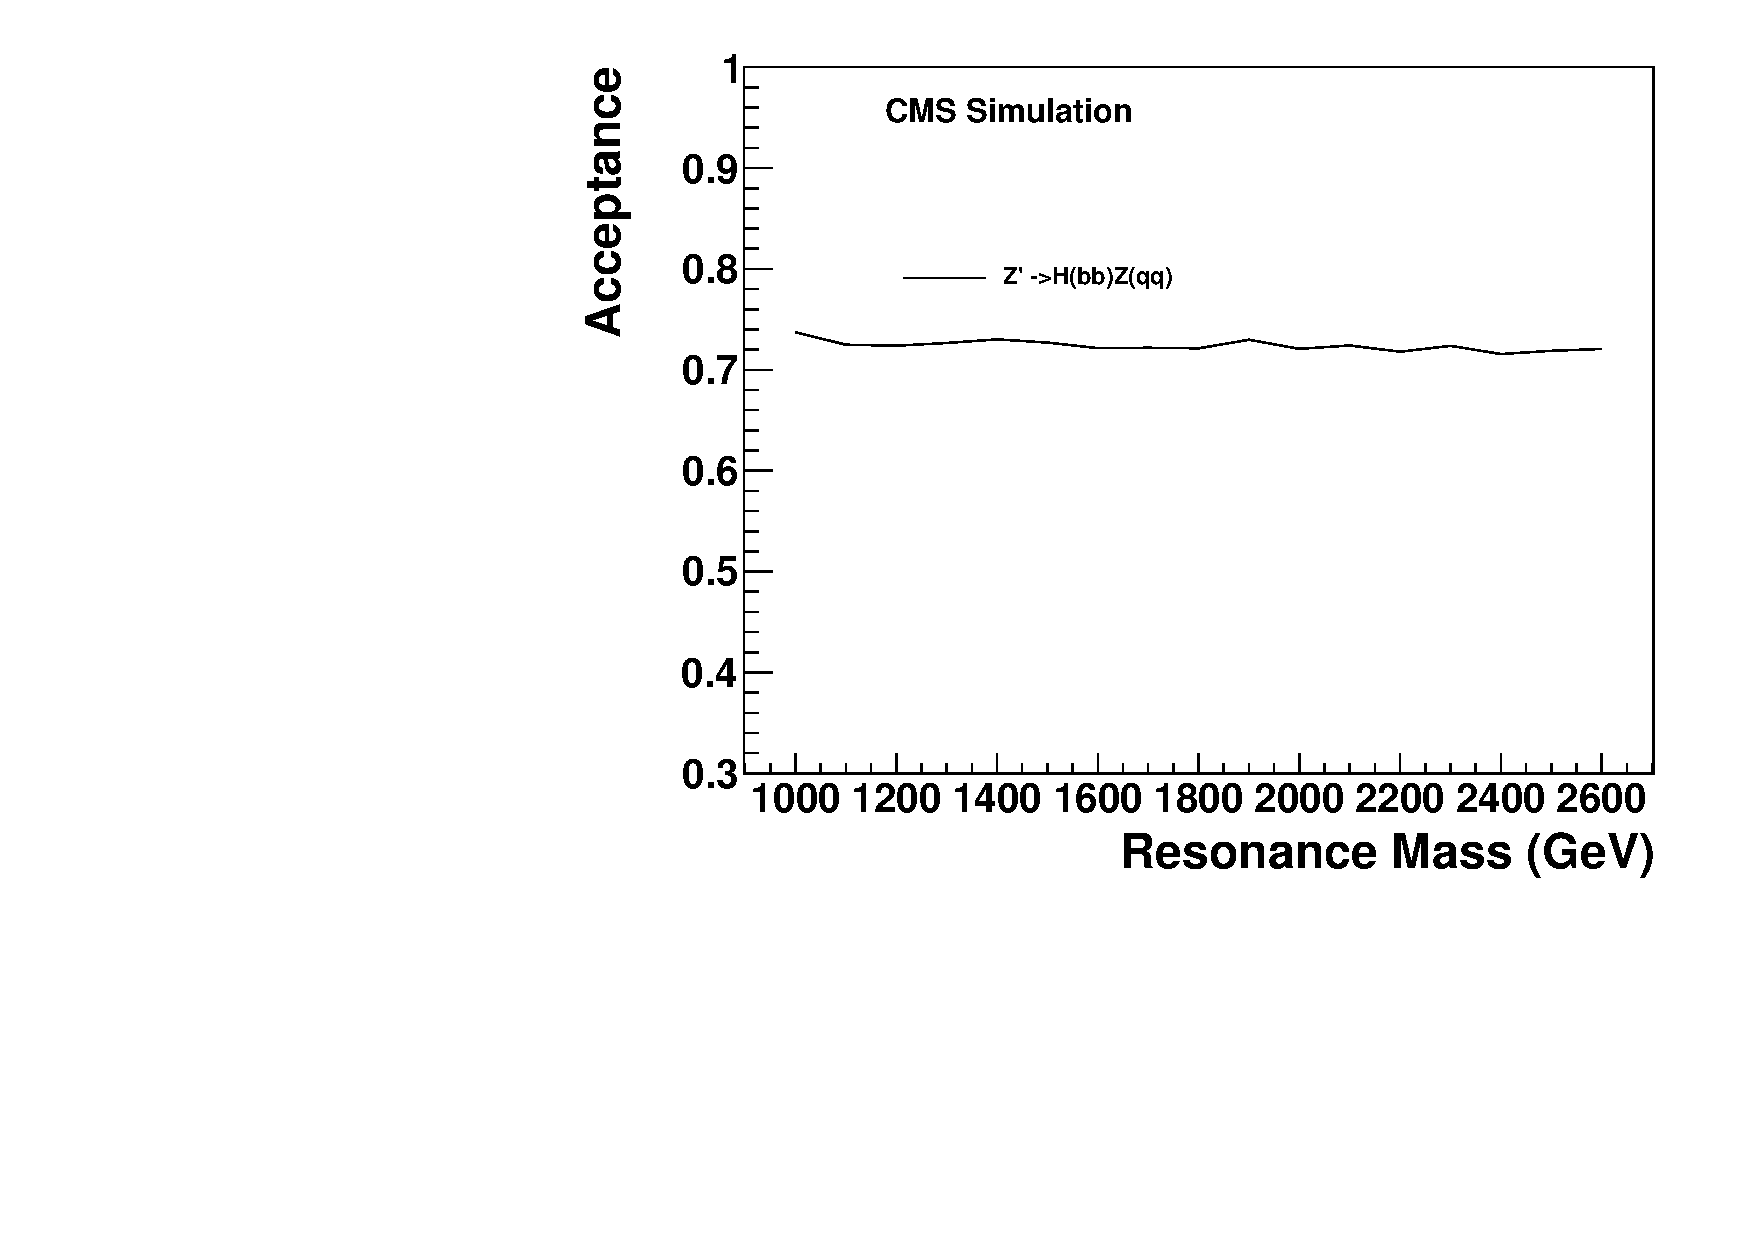
\includegraphics[width=0.60\textwidth]{HbbZqqfigs/Signal/HbbZqq-signal-acc-8TeV.pdf}
\end{center}
\caption{
This is the overall Signal tagging efficiency on the H(bb) channel. 
}
\label{fig:HbbEff}
\end{figure}


\begin{figure}[htb]
\begin{center}
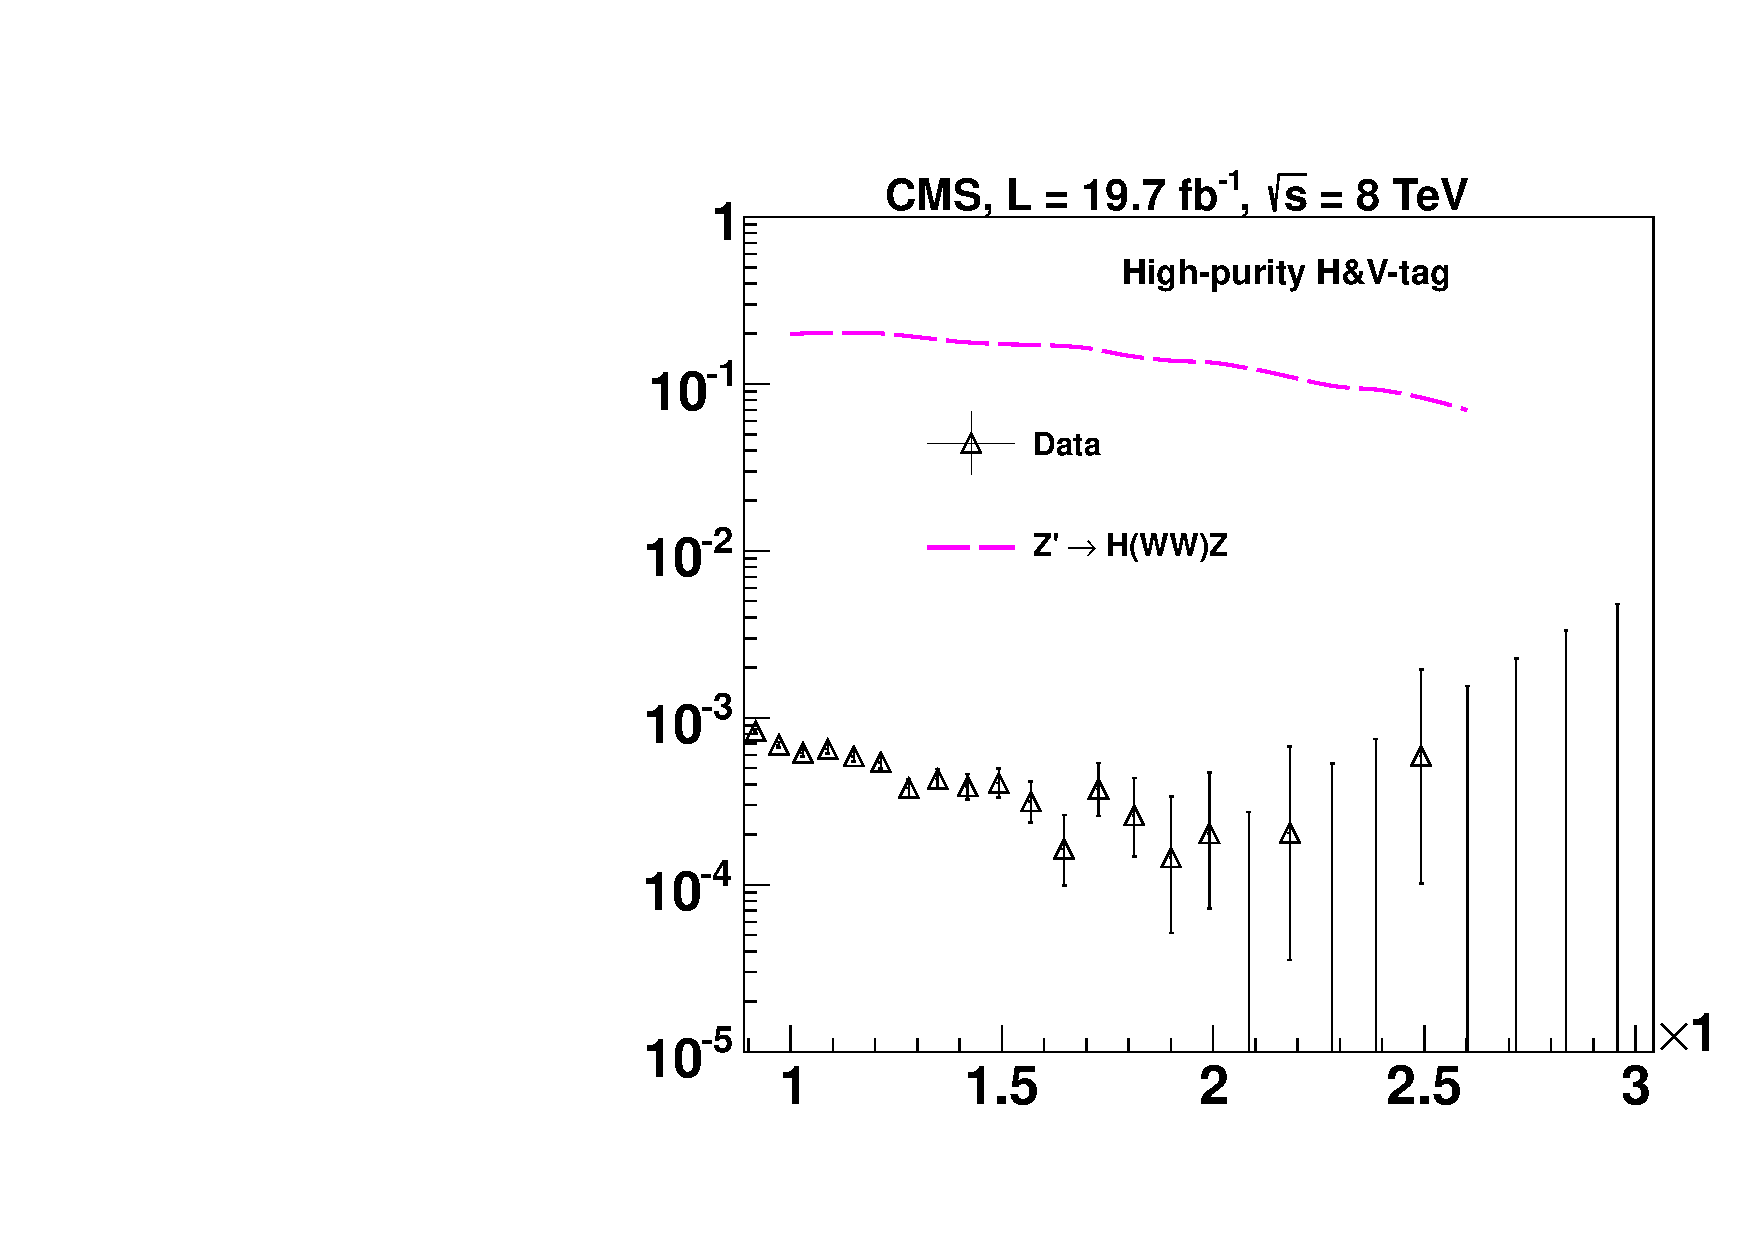
\includegraphics[width=0.33\textwidth]{HqqqqZqqfigs/Signal/tagging-eff-HighPuri.pdf}
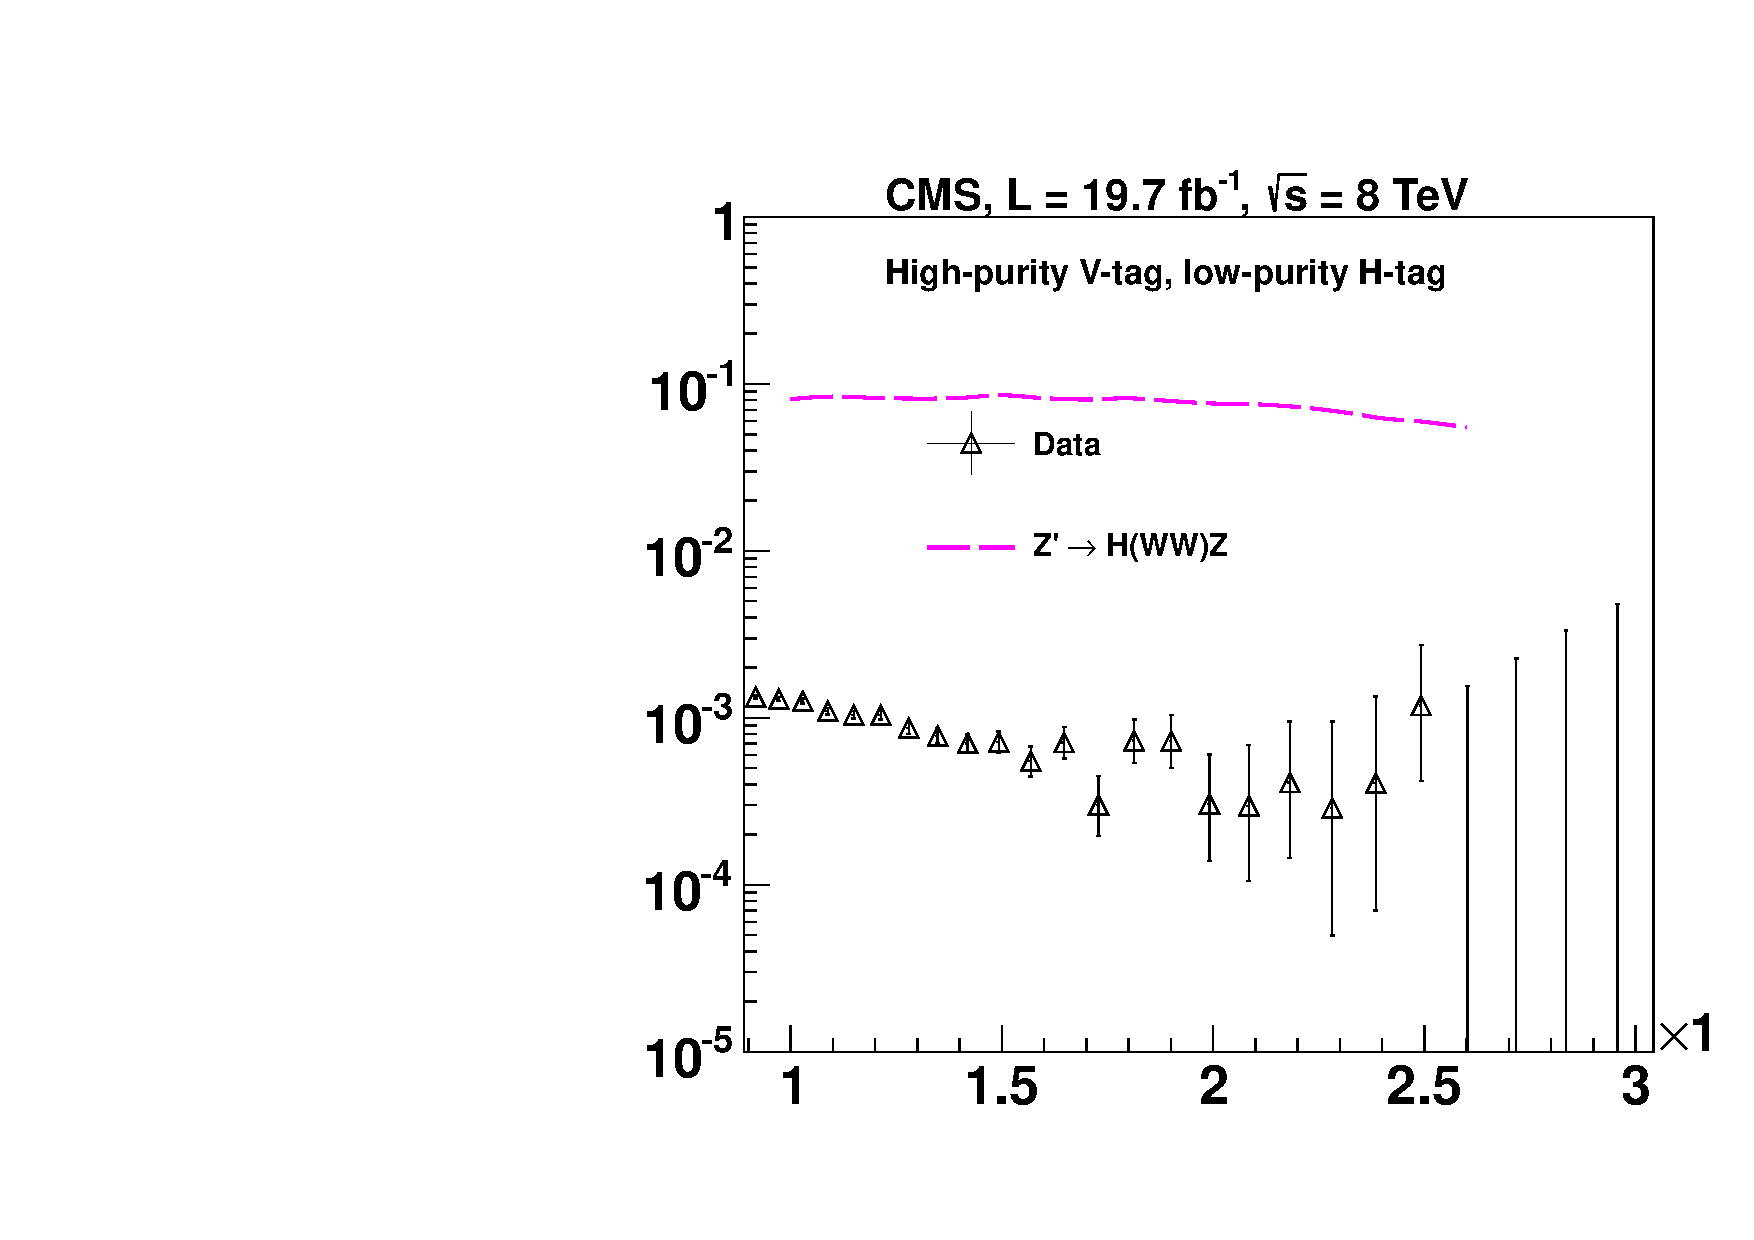
\includegraphics[width=0.33\textwidth]{HqqqqZqqfigs/Signal/tagging-eff-LowPuriH.pdf}
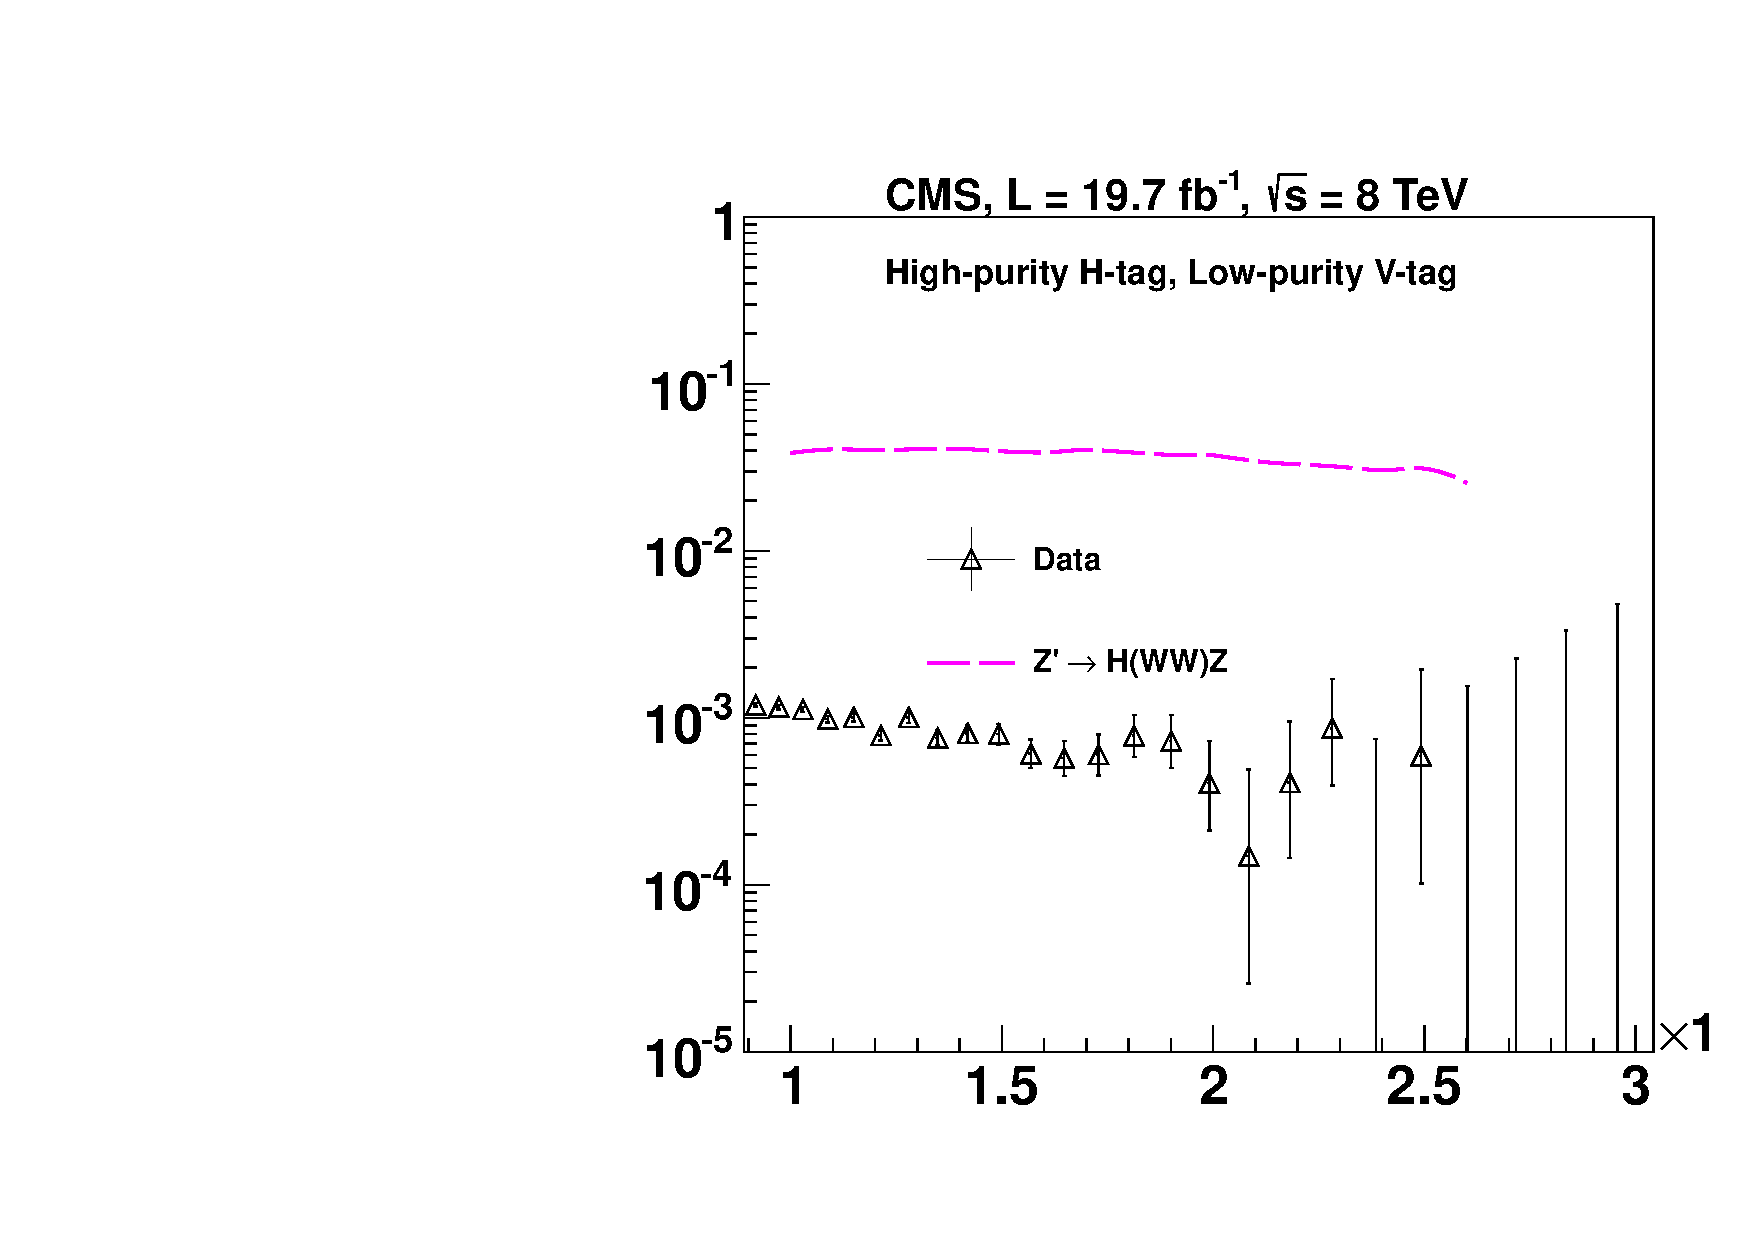
\includegraphics[width=0.33\textwidth]{HqqqqZqqfigs/Signal/tagging-eff-LowPuriV.pdf}
\end{center}
\caption{
This is the overall Signal tagging efficiency on the H(ww) channel. 
}
\label{fig:HwwEff}
\end{figure}







\iffalse

The full event selection efficiency is estimated using simulated
signal samples.
Less than 1\% of the $\cPZ\cPZ$ or $\PW\PW$ events which pass the full
selection are from $\cPZ\cPZ \to ll qq$ or $\PW\PW \to l\nu qq$
decays, where $l$ can be a muon or electron.  While 3\% of the
selected $\cPZ\cPZ$ events are from $\cPZ\cPZ \to \tau\tau qq$ decays,
less than 1\% of the selected $\PW\PW$ events are from $\PW\PW \to
\tau\nu qq$ decays.
To within 10\% accuracy the full selection efficiency can
therefore be
approximated by the product of the $\PW/\cPZ$-tagging efficiency
and an approximate acceptance.
This acceptance is shown in Fig.~\ref{fig:acceptances} and
takes into account the angular acceptance
($|\eta| < 2.5$, $|\Delta\eta|<1.3$),
the branching into quark final states,
BR($\PW/\cPZ \to \text{quarks}$) and a matching within
$\Delta R = \sqrt{(\Delta \eta)^2 + (\Delta\phi)^2} <0.5$
between the generated W/Z bosons and the reconstructed jets.


%\begin{table}[htbp]
%\begin{tabular}{|l|l|r|r|l|l|r|r|}
%\hline
%signal  & model & mass & BR($W/Z \to jets$)$\times$acc. & M 1-tag & H 1-tag & M 2-tag & H 2-tag \\ \hline
%$G_{RS} \to WW$ & Herwig++ & 1000 & 0.382 & NAN & NAN & 0.073 & 0.116 \\ 
%$G_{RS} \to WW$ & Herwig++ & 1500 & 0.401 & NAN & NAN & 0.076 & 0.092 \\ 
%$G_{RS} \to WW$ & Herwig++ & 1800 & 0.403 & NAN & NAN & 0.082 & 0.089 \\ 
%$G_{RS} \to WW$ & Herwig++ & 2000 & 0.404 & NAN & NAN & 0.076 & 0.079 \\ 
%$G_{RS} \to WW$ & Herwig++ & 2500 & 0.411 & NAN & NAN & 0.055 & 0.046 \\ 
%$G_{RS} \to WW$ & Herwig++ & 3000 & 0.409 & NAN & NAN & 0.032 & 0.029 \\ \hline 
%$G_{RS} \to ZZ$ & Herwig++ & 1000 & 0.390 & NAN & NAN & 0.070 & 0.120 \\ 
%$G_{RS} \to ZZ$ & Herwig++ & 1500 & 0.391 & NAN & NAN & 0.088 & 0.119 \\ 
%$G_{RS} \to ZZ$ & Herwig++ & 1800 & 0.387 & NAN & NAN & 0.095 & 0.125 \\ 
%$G_{RS} \to ZZ$ & Herwig++ & 2000 & 0.383 & NAN & NAN & 0.095 & 0.121 \\ 
%$G_{RS} \to ZZ$ & Herwig++ & 3000 & 0.374 & NAN & NAN & 0.077 & 0.056 \\ \hline
%$G_{RS} \to WW$ & Pythia Z2* & 1000 & 0.455 & NAN & NAN & 0.081 & 0.132 \\ 
%$G_{RS} \to WW$ & Pythia Z2* & 1500 & 0.432 & NAN & NAN & 0.088 & 0.124 \\ 
%$G_{RS} \to WW$ & Pythia Z2* & 1800 & 0.419 & NAN & NAN & 0.079 & 0.109 \\ 
%$G_{RS} \to WW$ & Pythia Z2* & 2000 & 0.415 & NAN & NAN & 0.078 & 0.094 \\ 
%$G_{RS} \to WW$ & Pythia Z2* & 2500 & 0.397 & NAN & NAN & 0.059 & 0.056 \\ 
%$G_{RS} \to WW$ & Pythia Z2* & 3000 & 0.391 & NAN & NAN & 0.040 & 0.035 \\ \hline
%$G_{RS} \to ZZ$ & Pythia Z2* & 1000 & 0.454 & NAN & NAN & 0.075 & 0.149 \\ 
%$G_{RS} \to ZZ$ & Pythia Z2* & 1500 & 0.417 & NAN & NAN & 0.106 & 0.161 \\ 
%$G_{RS} \to ZZ$ & Pythia Z2* & 1800 & 0.400 & NAN & NAN & 0.107 & 0.154 \\ 
%$G_{RS} \to ZZ$ & Pythia Z2* & 2000 & 0.389 & NAN & NAN & 0.113 & 0.148 \\ 
%$G_{RS} \to ZZ$ & Pythia Z2* & 3000 & 0.355 & NAN & NAN & 0.081 & 0.071 \\ \hline
%$W' \to WZ$ & Pythia Z2* & 1000 & 0.486 & NAN & NAN & 0.109 & 0.246 \\ 
%$W' \to WZ$ & Pythia Z2* & 1500 & 0.487 & NAN & NAN & 0.121 & 0.246 \\ 
%$W' \to WZ$ & Pythia Z2* & 1800 & 0.485 & NAN & NAN & 0.119 & 0.216 \\ 
%$W' \to WZ$ & Pythia Z2* & 2000 & 0.484 & NAN & NAN & 0.117 & 0.199 \\ 
%$W' \to WZ$ & Pythia Z2* & 2200 & 0.479 & NAN & NAN & 0.108 & 0.172 \\ 
%$W' \to WZ$ & Pythia Z2* & 2500 & 0.485 & NAN & NAN & 0.092 & 0.139 \\ 
%$W' \to WZ$ & Pythia Z2* & 3000 & 0.494 & NAN & NAN & 0.068 & 0.114 \\ \hline
%$q* \to qW$ & Pythia Z2* & 1000 & 0.502 & 0.125 & 0.364 & NAN & NAN \\ 
%$q* \to qW$ & Pythia Z2* & 1500 & 0.495 & 0.135 & 0.333 & NAN & NAN \\ 
%$q* \to qW$ & Pythia Z2* & 2000 & 0.497 & 0.139 & 0.306 & NAN & NAN \\ 
%$q* \to qW$ & Pythia Z2* & 3000 & 0.490 & 0.129 & 0.177 & NAN & NAN \\ 
%$q* \to qW$ & Pythia Z2* & 4000 & 0.475 & 0.121 & 0.130 & NAN & NAN \\ \hline
%$ q* \to qZ$ & Pythia Z2* & 1000 & 0.494 & 0.116 & 0.371 & NAN & NAN \\ 
%$ q* \to qZ$ & Pythia Z2* & 1500 & 0.488 & 0.138 & 0.384 & NAN & NAN \\ 
%$ q* \to qZ$ & Pythia Z2* & 2000 & 0.474 & 0.154 & 0.364 & NAN & NAN \\ 
%$ q* \to qZ$ & Pythia Z2* & 3000 & 0.452 & 0.173 & 0.262 & NAN & NAN \\ 
%$ q* \to qZ$ & Pythia Z2* & 4000 & 0.449 & 0.156 & 0.187 & NAN & NAN \\ \hline
%\end{tabular}
%\caption{Summary of signal branching ratio times angular acceptance and W/Z-tagging efficiency, in medium purity 1-tag, high purity 
%1-tag, medium purity 2-tag and high purity 2-tag categories. }
%\label{table:acceptance}
%\end{table}
%






%\begin{table}[htb]
%\begin{center}
%\begin{tabular}{ |c|c|c|c|c|c| }
%\hline
%signal & model & mass & BR($W/Z \to jets$)$\times$acc. & 1 W/Z-tag & 2 W/Z-tag\\
%\hline
%hline
%\end{tabular} 
%\end{center}
%\caption{Summary of signal branching ratio times acceptance and W/Z-tagging efficiency.}
%\label{table:acceptance}
%\end{table}

\begin{figure}[htb]
\begin{center}
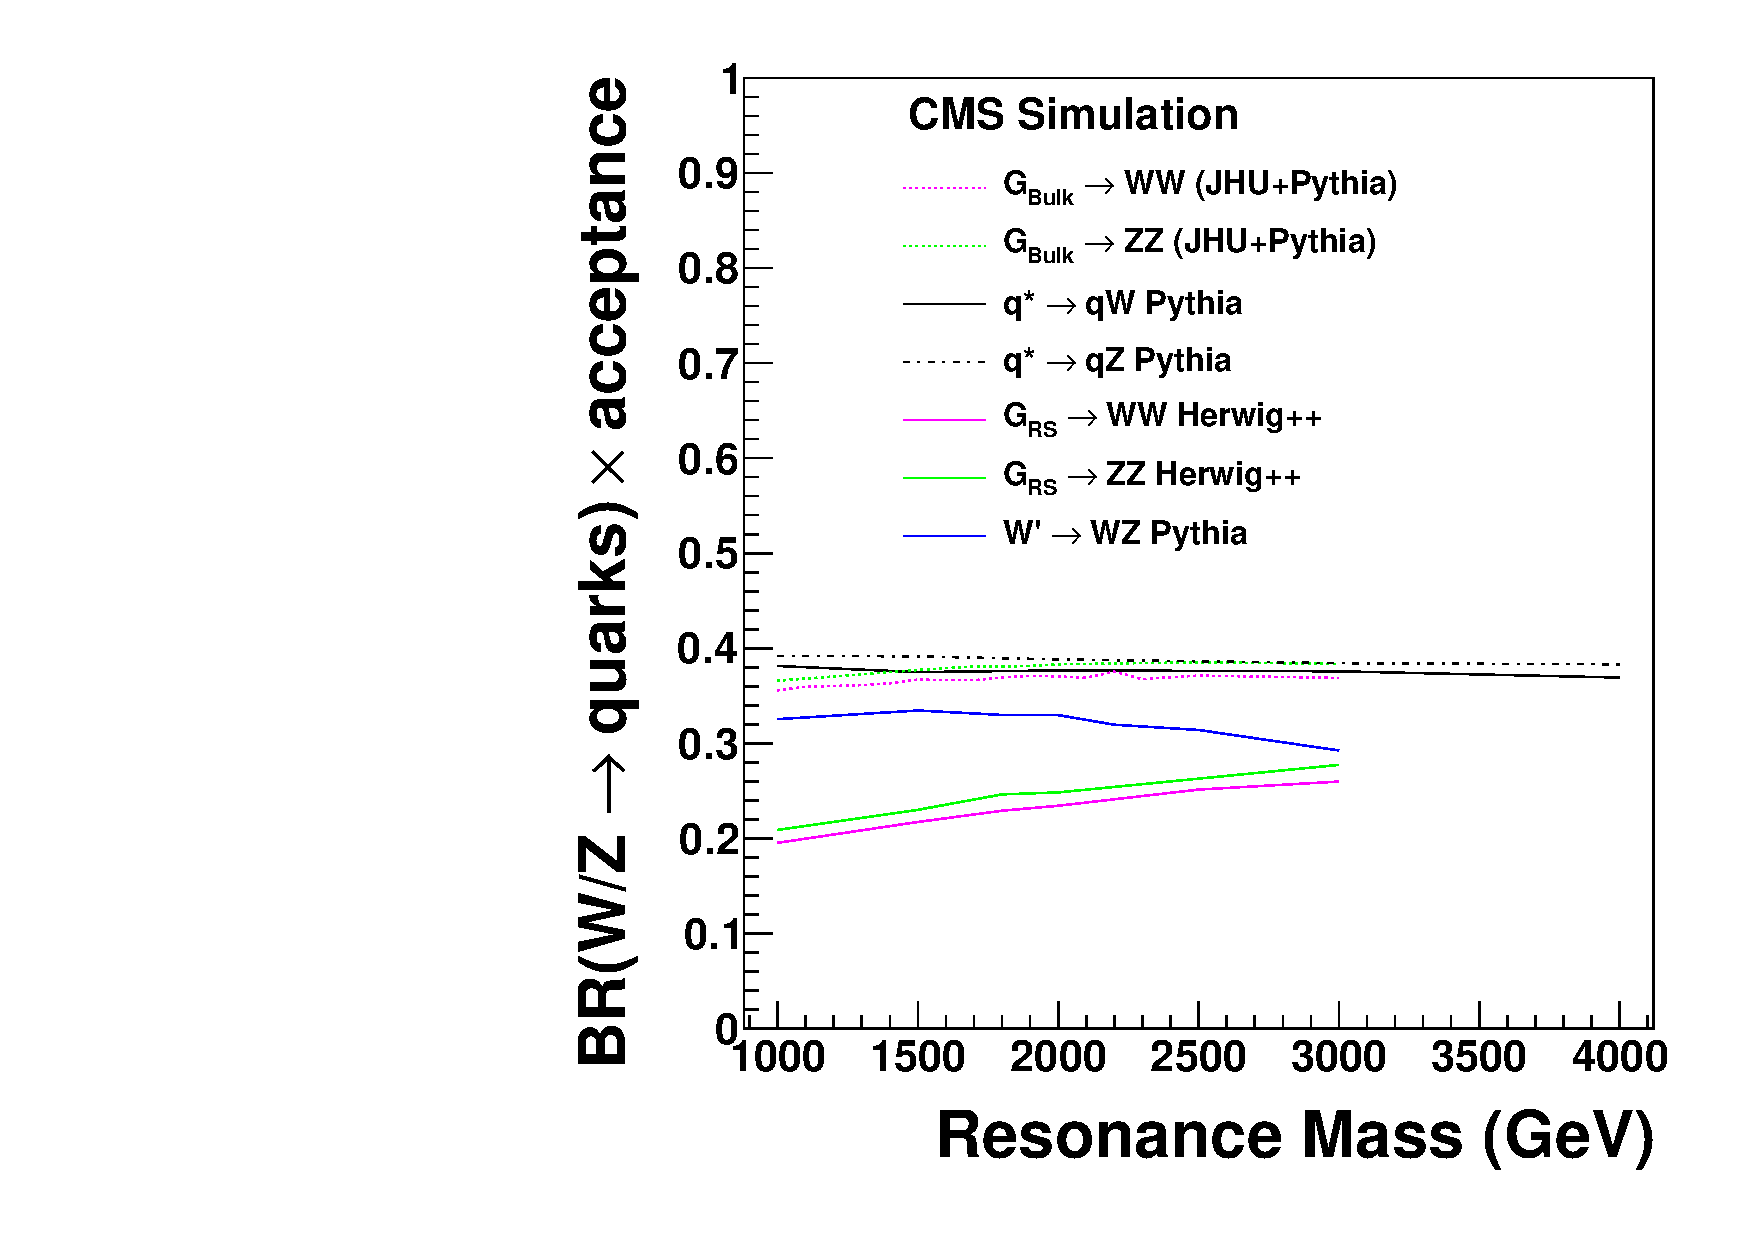
\includegraphics[width=0.88\textwidth]{figs/signal-acc-eff/all-signal-acc-8TeV.pdf}
\end{center}
\caption{Fraction of events with branching into quark final states, BR($\PW/\cPZ \to \text{quarks}$),
  which are reconstructed as dijets ($\text{quarks} \to \text{jets}$)
  and pass the angular acceptance ($|\eta| < 2.5$, $|\Delta\eta|<1.3$.}
\label{fig:acceptances}
\end{figure}

\begin{figure}[htb]
\begin{center}
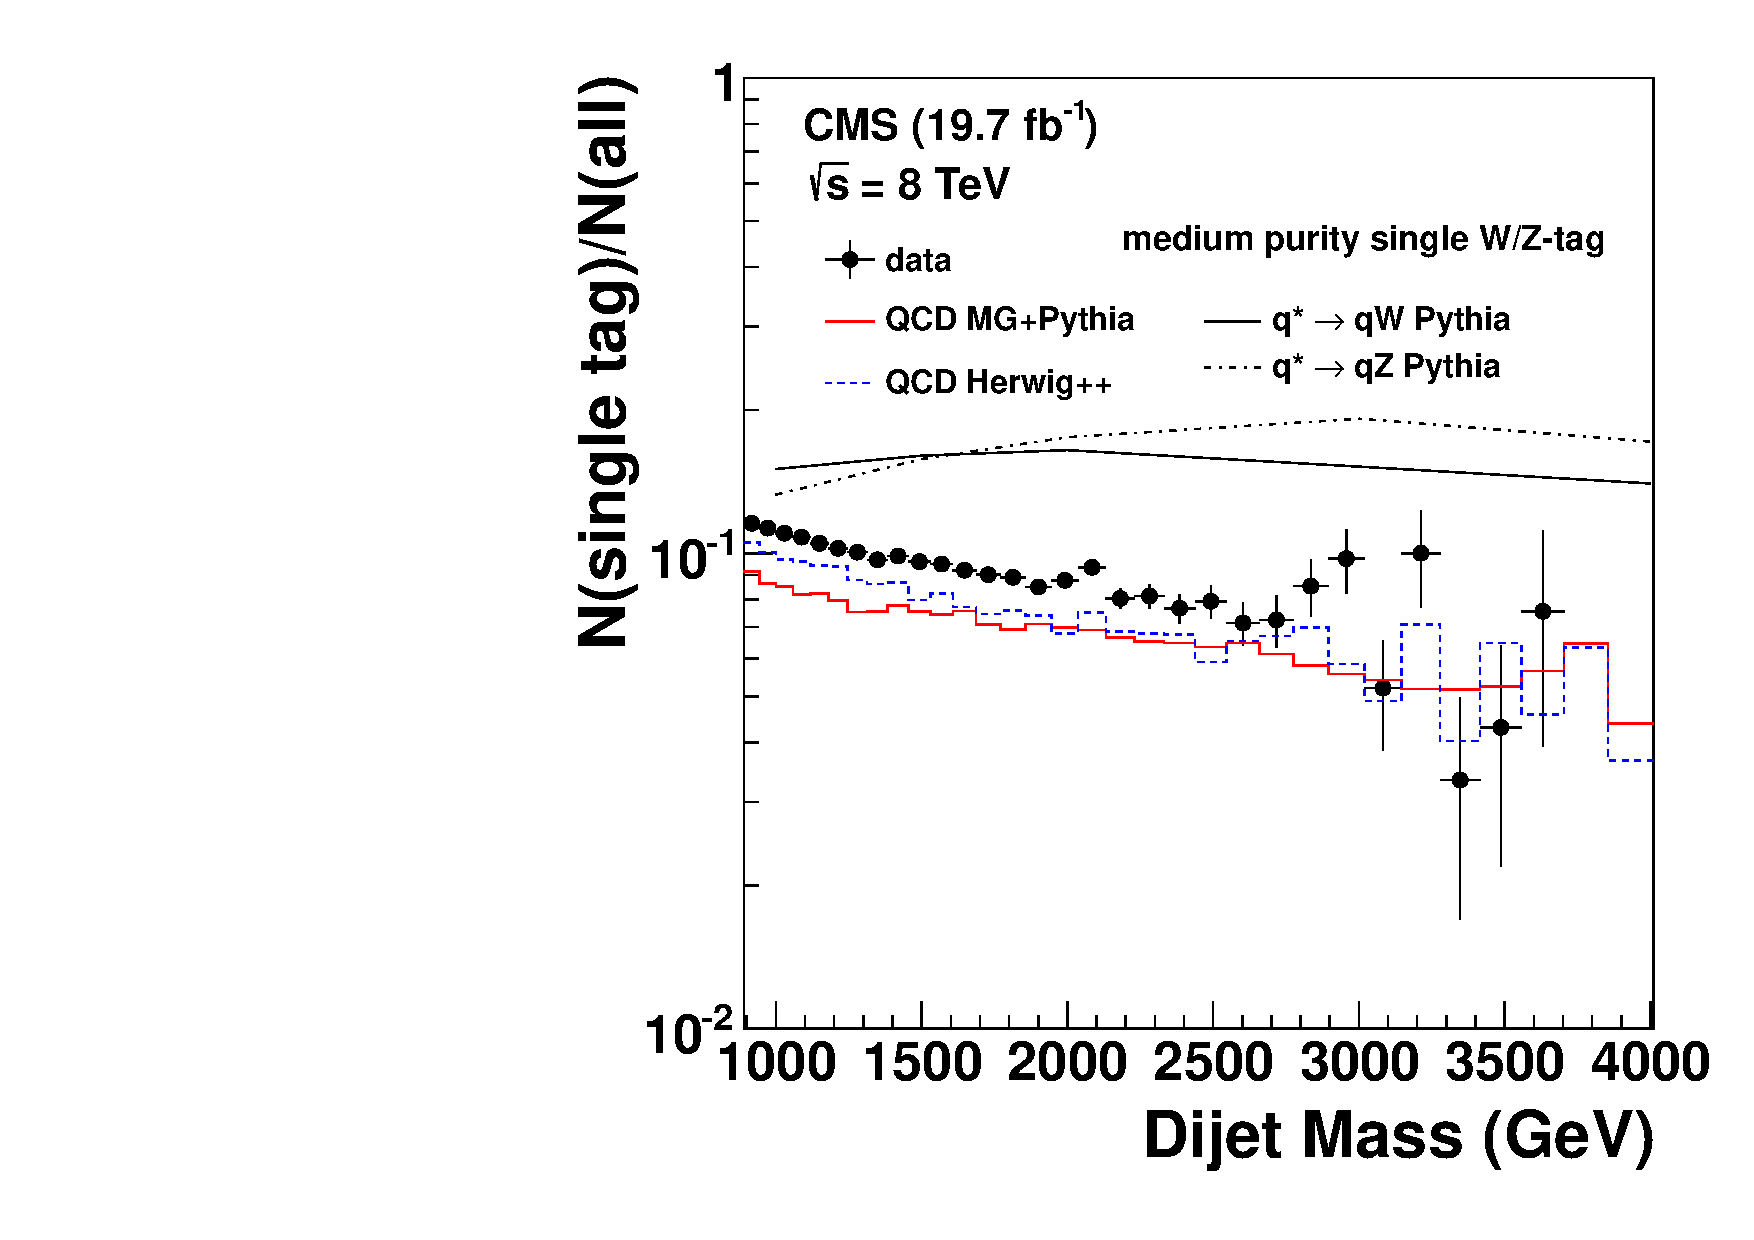
\includegraphics[width=0.49\textwidth]{figs/signal-acc-eff/single-tagging-eff-medium.pdf}
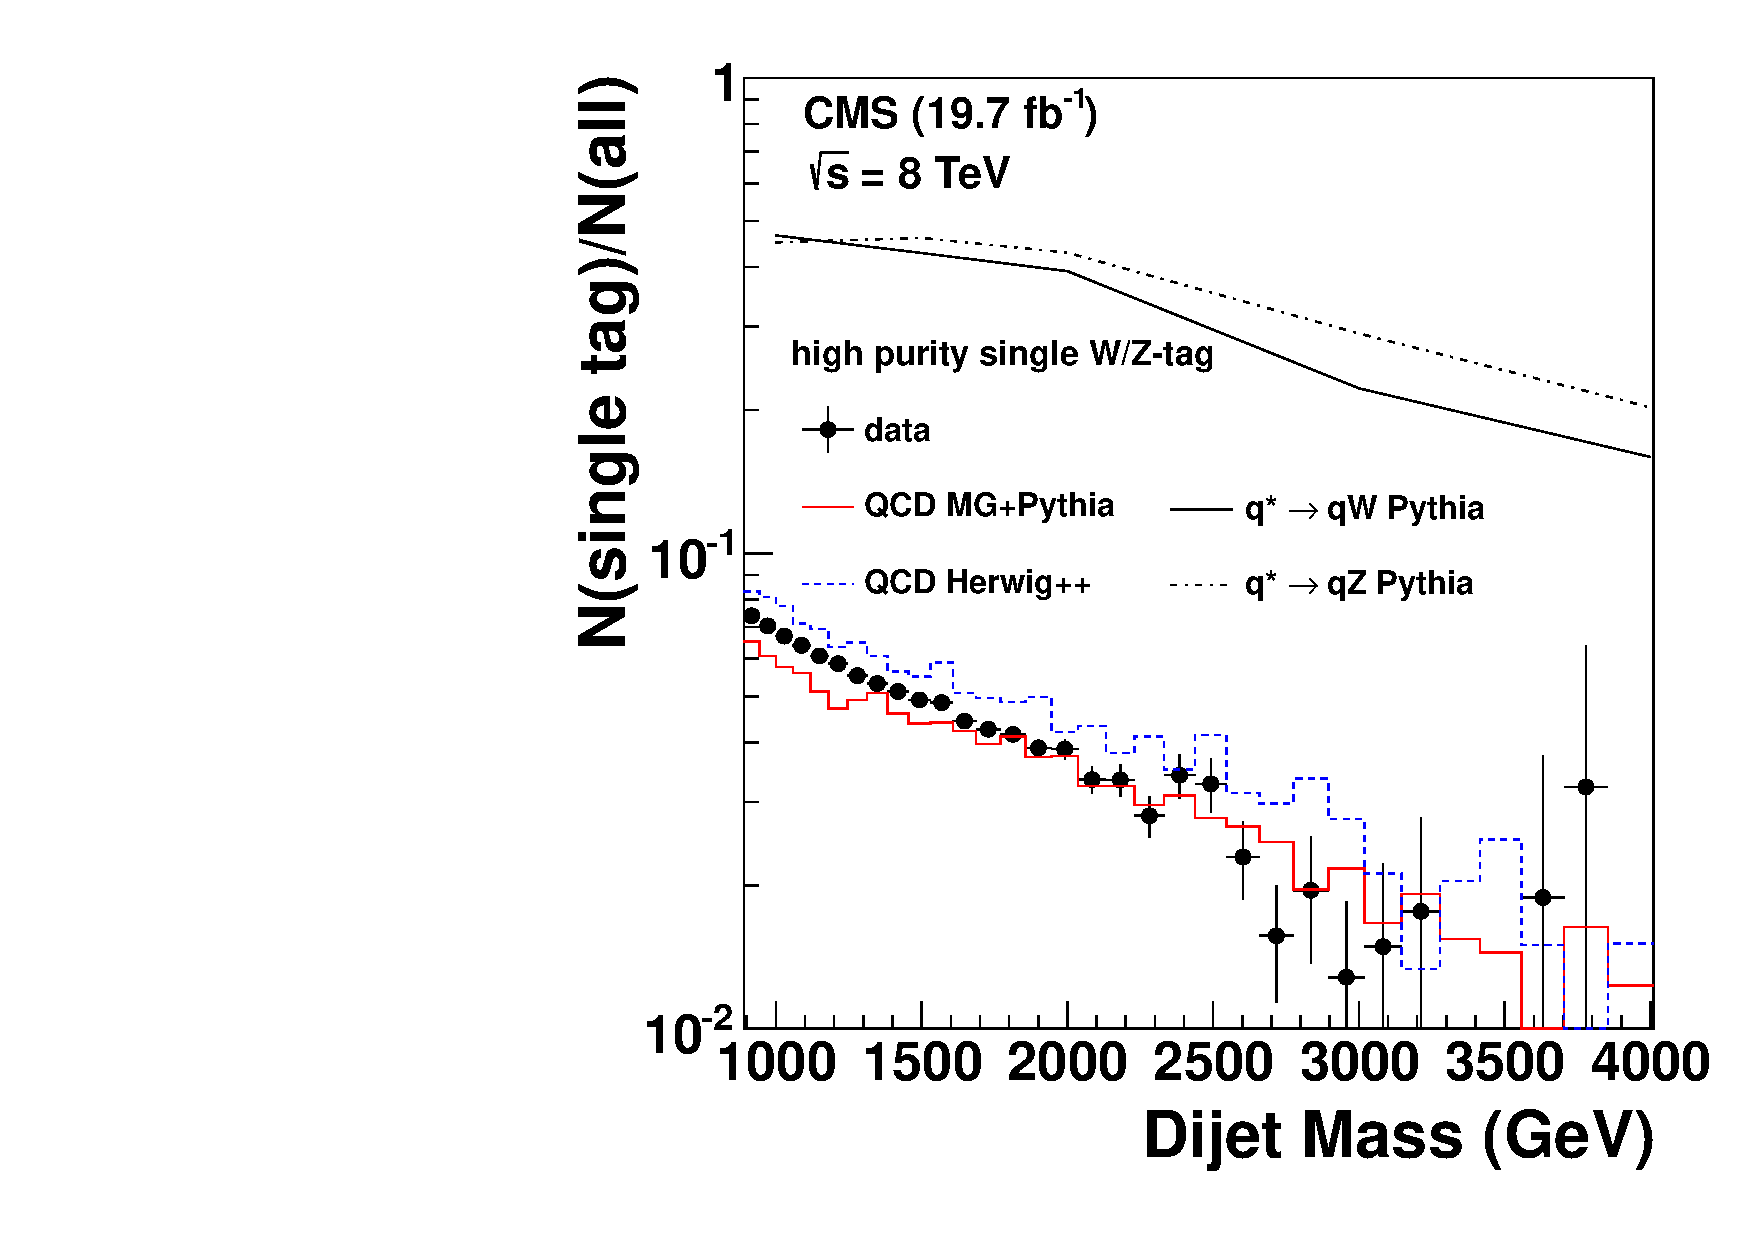
\includegraphics[width=0.49\textwidth]{figs/signal-acc-eff/single-tagging-eff.pdf}
\end{center}
\caption{The fraction of singly-tagged events, requiring one medium purity (left) 
  and high purity (right) $\PW/\cPZ$-tag in data,
  signal and background simulations for events passing the angular acceptance
  requirement ($|\eta| < 2.5$, $|\Delta\eta|<1.3$).}
\label{fig:singleefficiencies}
\end{figure}

\begin{figure}[htb]
\begin{center}
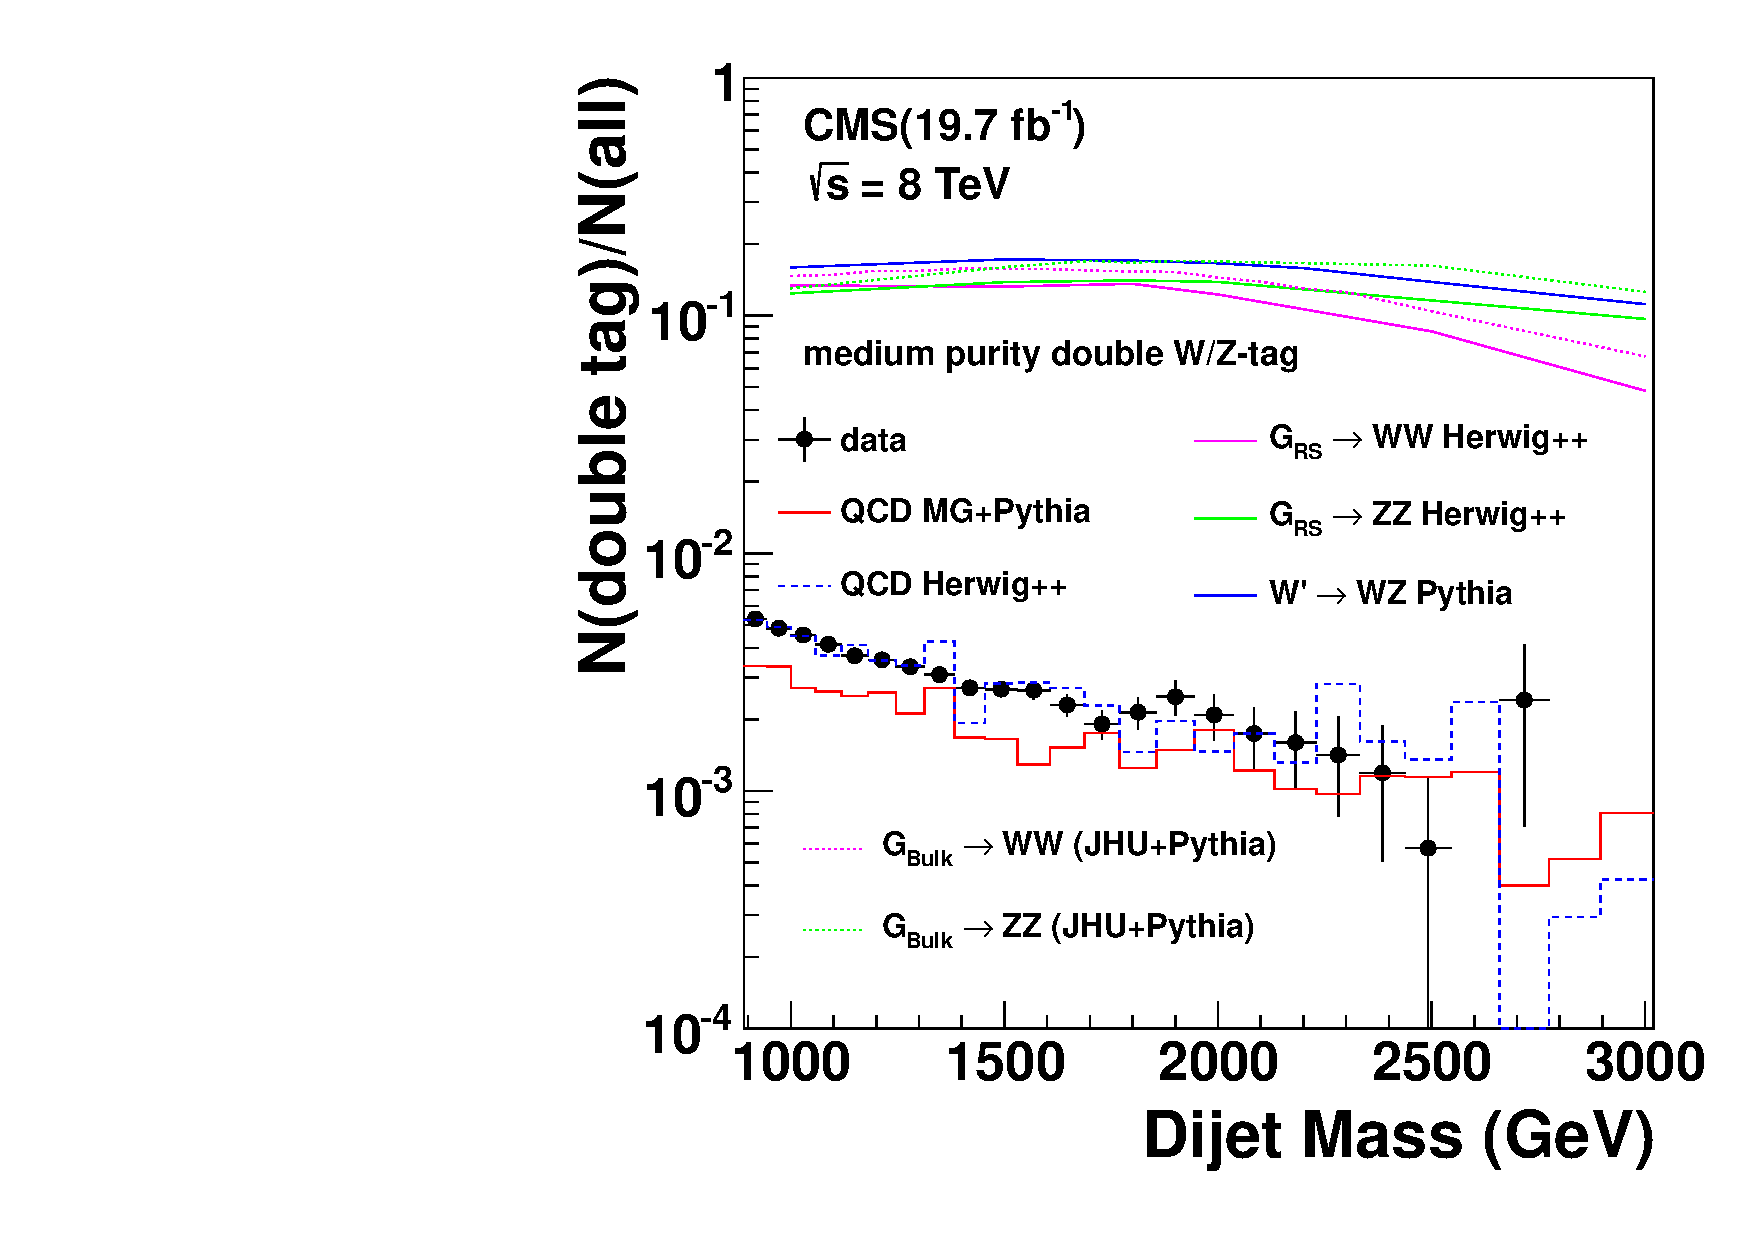
\includegraphics[width=0.49\textwidth]{figs/signal-acc-eff/double-tagging-eff-medium.pdf}
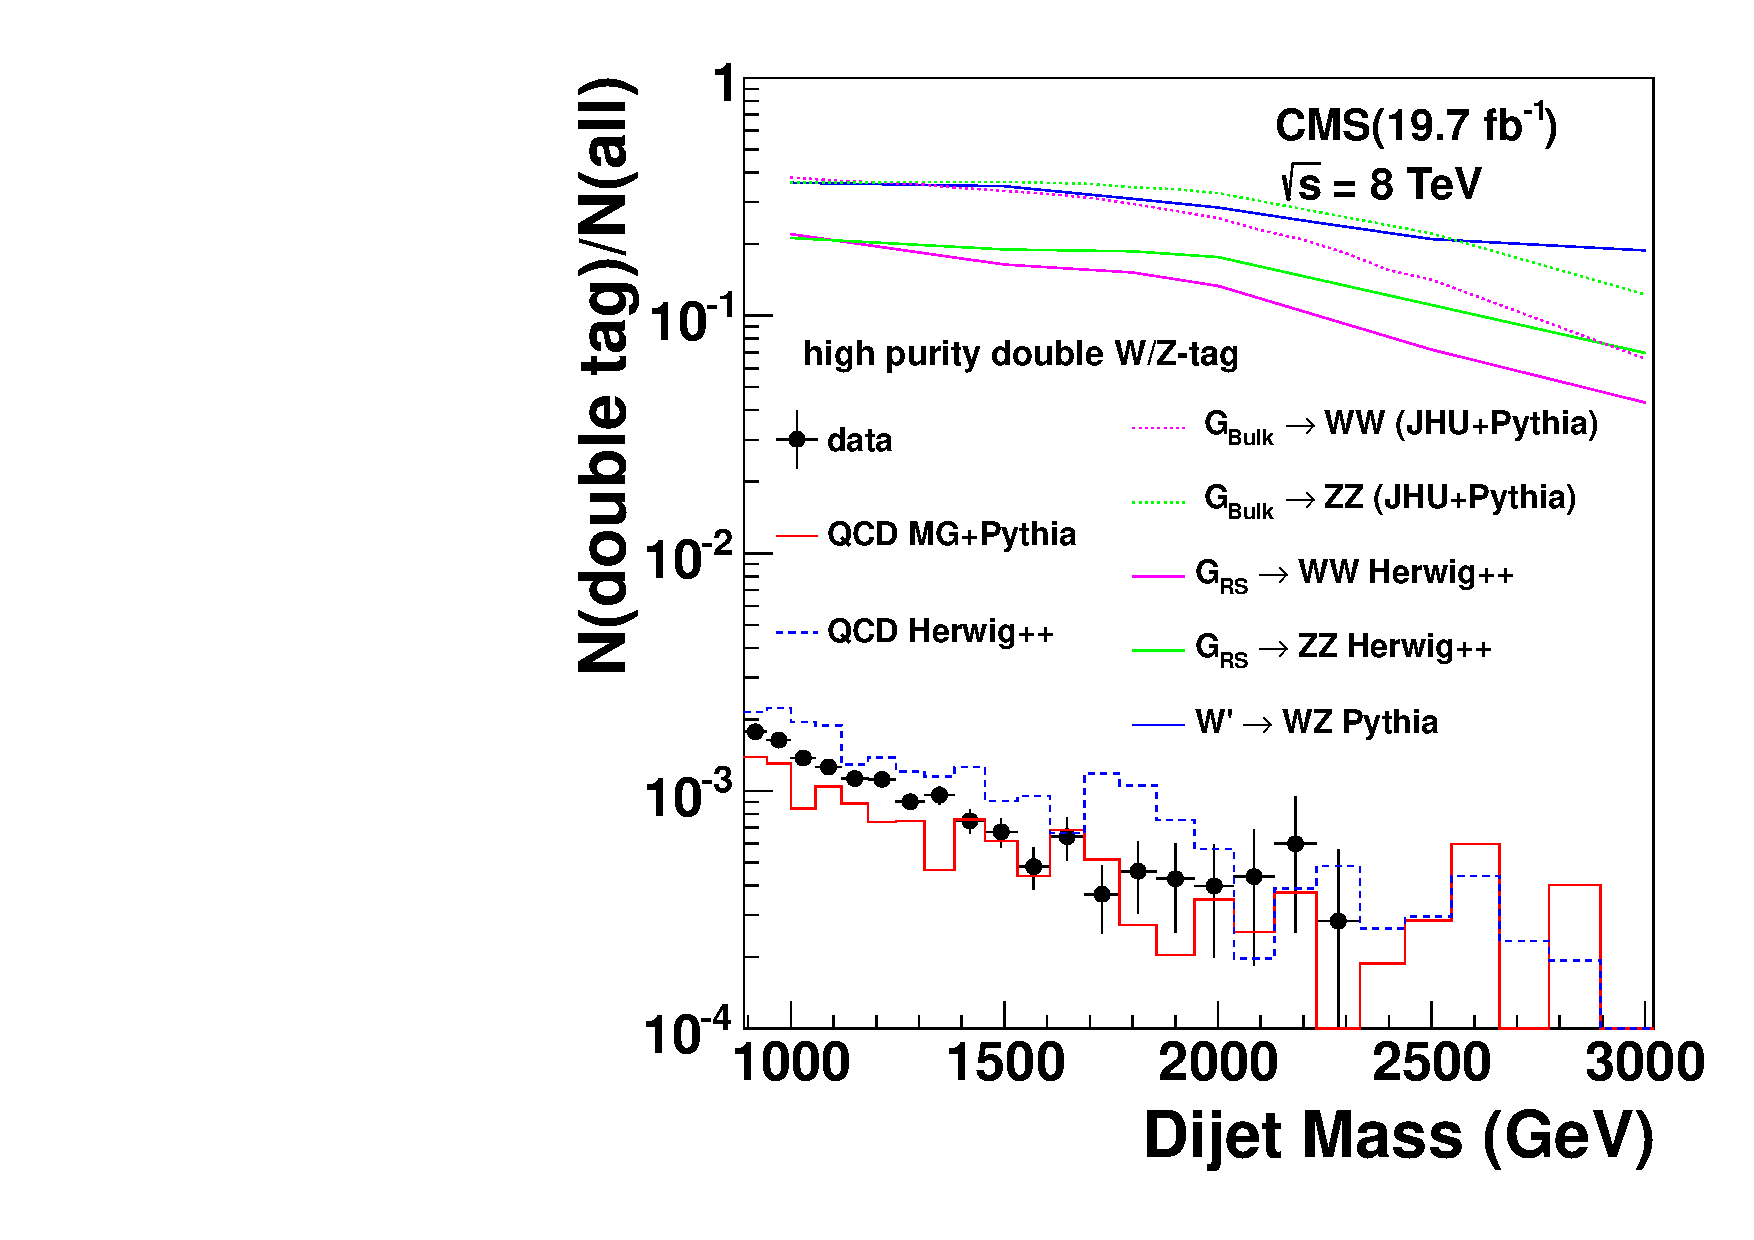
\includegraphics[width=0.49\textwidth]{figs/signal-acc-eff/double-tagging-eff.pdf}
\end{center}
\caption{The fraction of doubly-tagged events, requiring two medium purity (left) 
and high purity (right) $\PW/\cPZ$-tags in data,
  signal and background simulations for events passing the angular acceptance
  requirement ($|\eta| < 2.5$, $|\Delta\eta|<1.3$).}
\label{fig:doubleefficiencies}
\end{figure}
%


The W/Z-tagging efficiency is shown in Fig.~\ref{fig:singleefficiencies} and Fig.~\ref{fig:doubleefficiencies}.
%The W/Z-tagging efficiency for single W/Z-tagged signals is about $13\% - 38\%$ in high purity category, and $12\% - 18\%$ in medium purity category.
%The W/Z-tagging efficiency for a double W/Z-tagged signals is about $3\% - 12\%$ in high purity category, and $3\% - 9\%$ in medium purity category.


The signal shapes for all five processes considered in this analysis are shown in Fig.~\ref{fig:mediumsignalShapes} and Fig.~\ref{fig:highsignalShapes}.  
For the $qW$ and $qZ$ final states the shape with a single W/Z-tag required is shown, while for the other signals two W/Z-tags are required.


%Fig~\ref{fig:acceptanceGstarWWherwig} and Fig~\ref{fig:acceptanceGstarWWpythia} show the signal shape for process: $G_{RS} \to WW$.
%Fig~\ref{fig:acceptanceGstarZZherwig} and Fig~\ref{fig:acceptanceGstarZZpythia} show the signal shape for process: $G_{RS} \to ZZ$.  
%Fig~\ref{fig:acceptanceWprime} shows the signal shape for process: $W' \to WZ$. 
%Fig~\ref{fig:acceptanceqstarqW} and Fig~\ref{fig:acceptanceqstarqZ} shows the signal shape for process: $q* \to qW$, $qZ$.
%The different line colors correspond to different signal resonance masses.
%The dashed line is for signal with a single W/Z-tag, while the dotted 
%line is for signal with two W/Z-tags.

\begin{figure}[htb]
\begin{center}
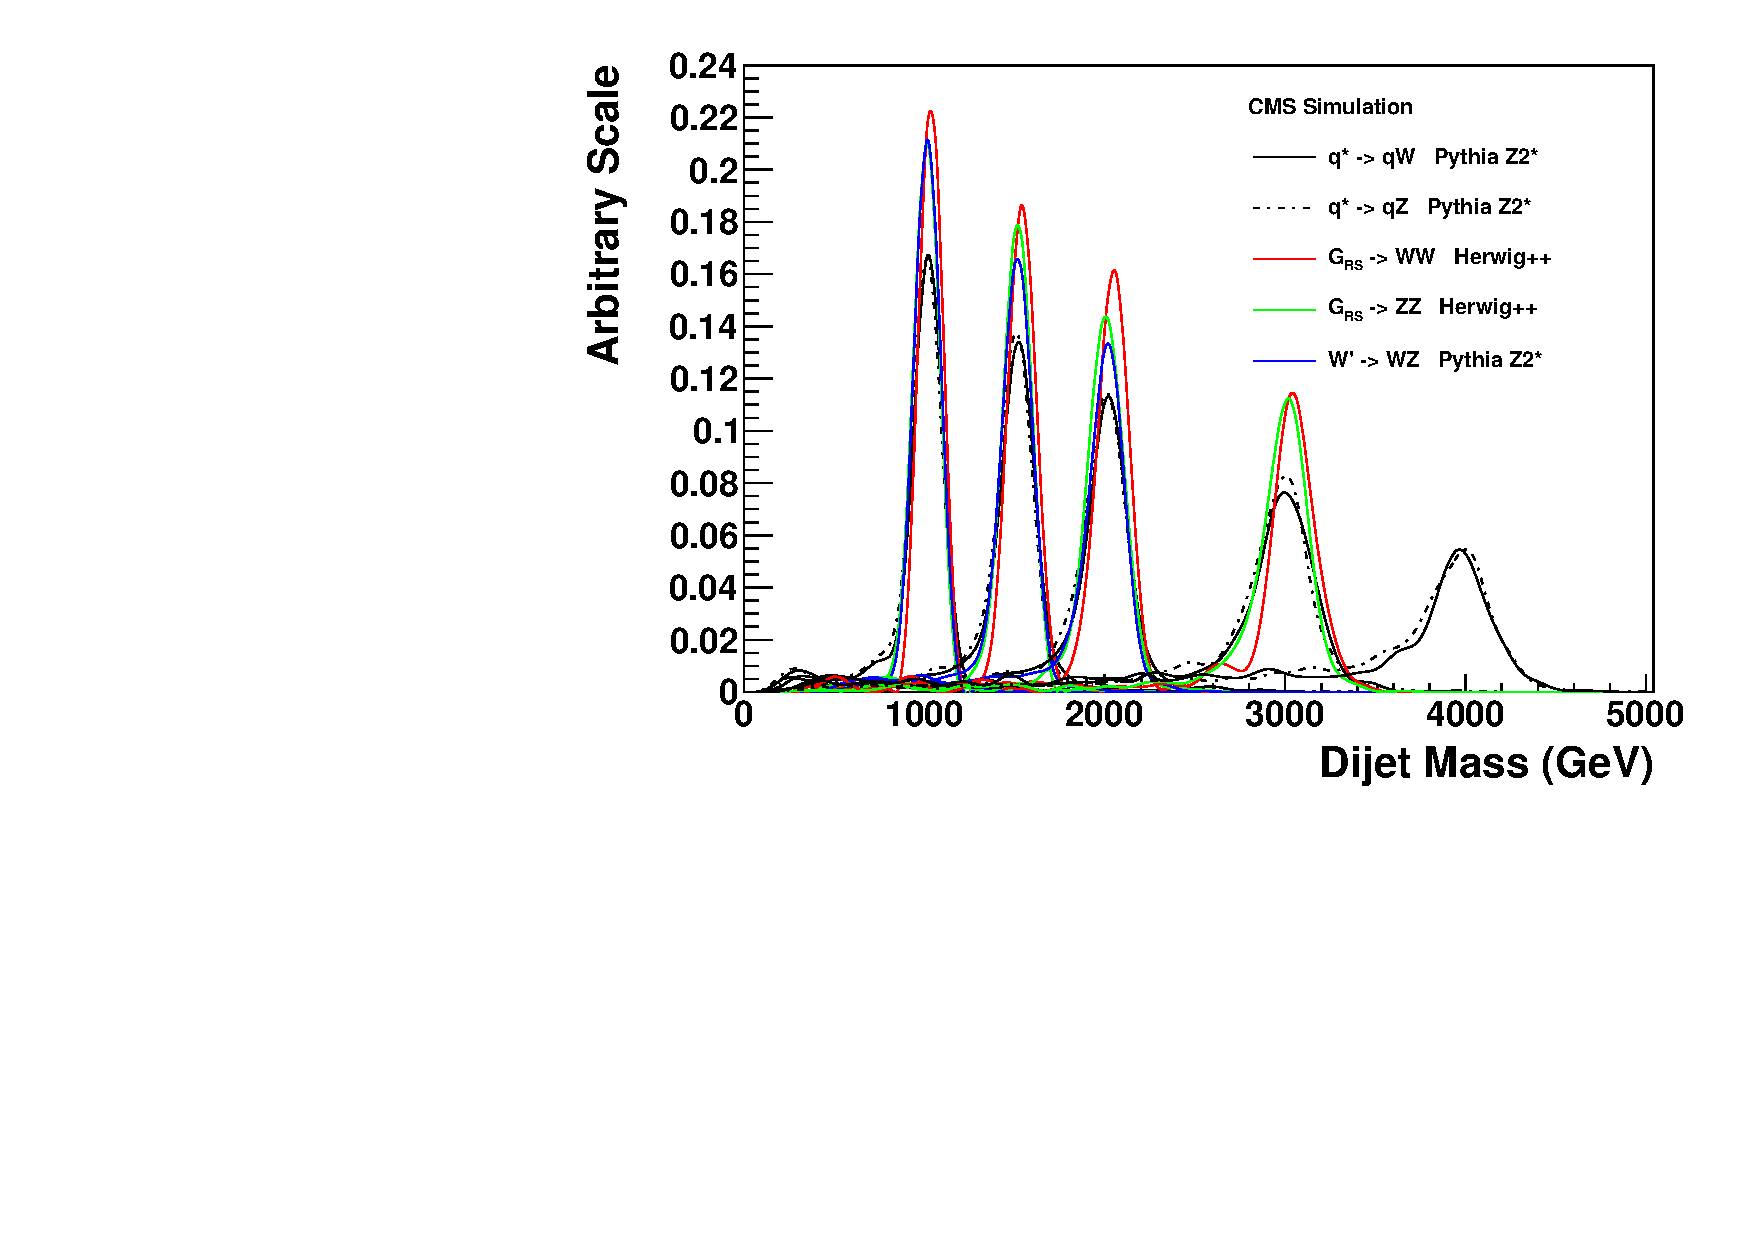
\includegraphics[width=0.75\textwidth]{figs/signal-acc-eff/resonance-shape-medium.pdf}
\end{center}
\caption{The normalized medium purity signal resonance distribution for  $G_{RS}\to \wboson\wboson$, $G_{RS}\to \zboson\zboson$, $W' \to WZ$, $q*\to qW$, and $q*\to qZ$ resonances of dijet invariant mass 1.0\TeVcc, 1.5\TeVcc, 2.0\TeVcc, 2.5 \TeVcc,  3.0\TeVcc, 4.0\TeVcc.
}
\label{fig:mediumsignalShapes}
\end{figure}


\begin{figure}[htb]
\begin{center}
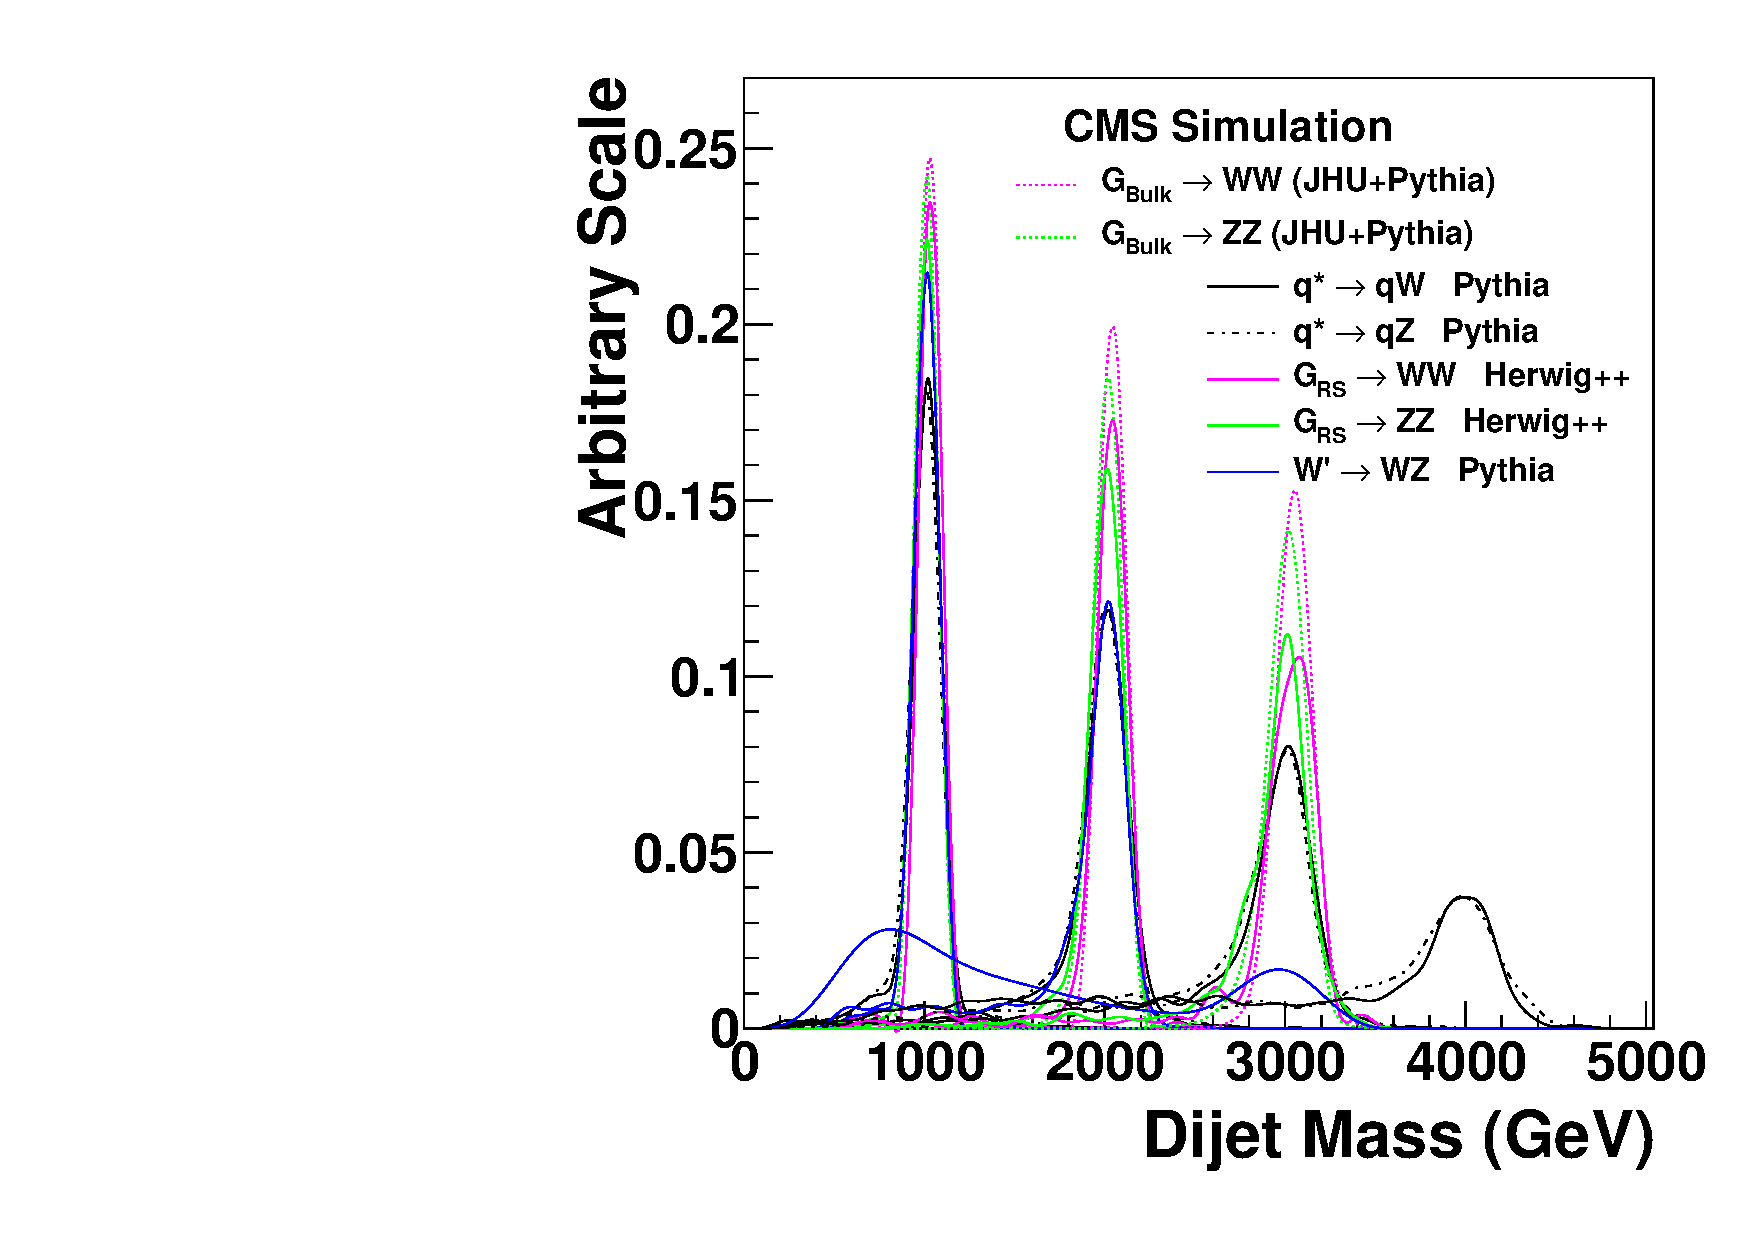
\includegraphics[width=0.75\textwidth]{figs/signal-acc-eff/resonance-shape.pdf}
\end{center}
\caption{The normalized high purity signal resonance distribution for  $G_{RS}\to \wboson\wboson$, $G_{RS}\to \zboson\zboson$, $W' \to WZ$, $q*\to qW$, and $q*\to qZ$ resonances of dijet invariant mass 1.0\TeVcc, 1.5\TeVcc, 2.0\TeVcc,  3.0\TeVcc, 4.0\TeVcc.
}
\label{fig:highsignalShapes}
\end{figure}

%\begin{figure}[htb]
%\begin{center}
%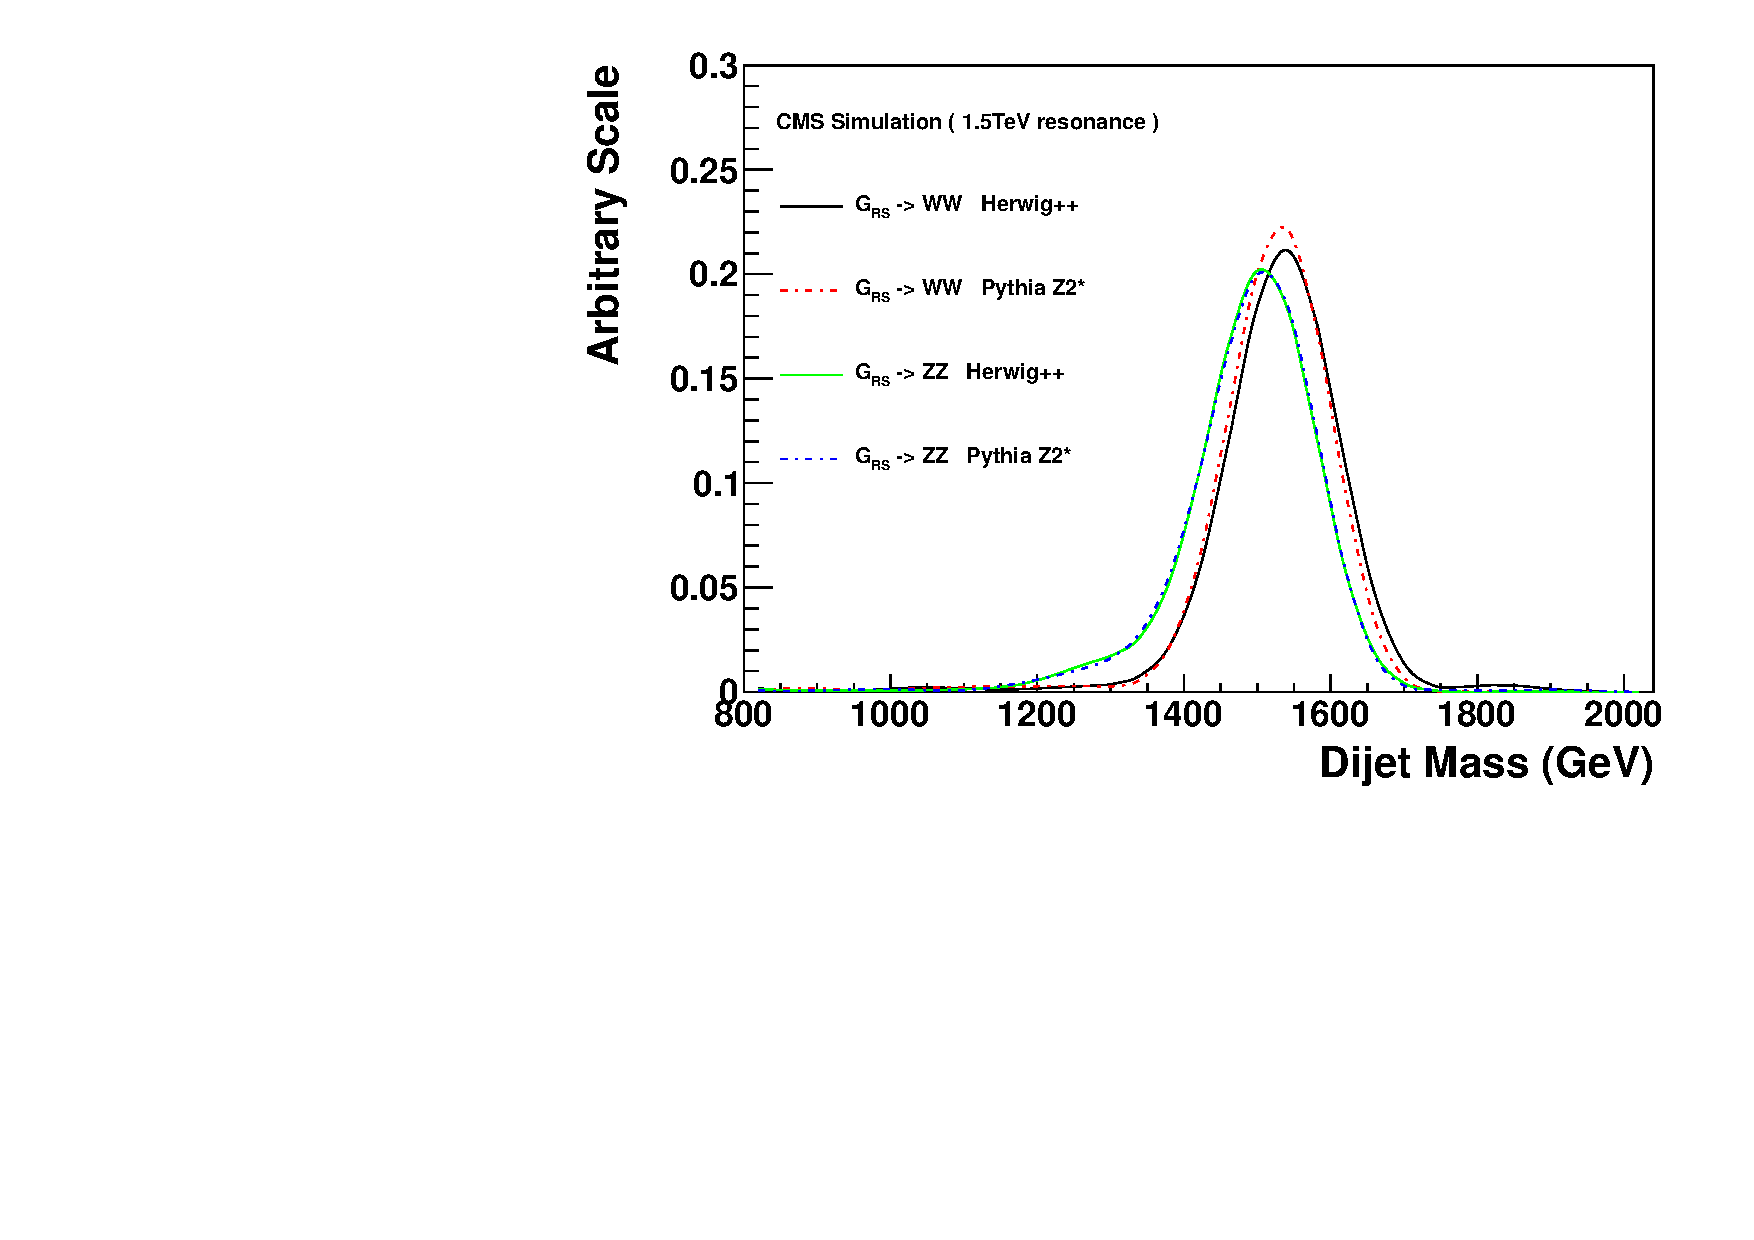
\includegraphics[width=0.75\textwidth]{figs/signal-acc-eff/resonance-shape-double-1500.pdf}
%\end{center}
%\caption{The normalized signal resonance distribution of Herwig++ and Pythia6 Z2* for 1.5 \TeVcc $G_{RS}\to \wboson\wboson$, $G_{RS}\to \zboson\zboson$ resonances of dijet invariant mass.
%}
%\label{fig:signalShapes2}
%\end{figure}




%\begin{figure}[htb]
%\begin{center}
%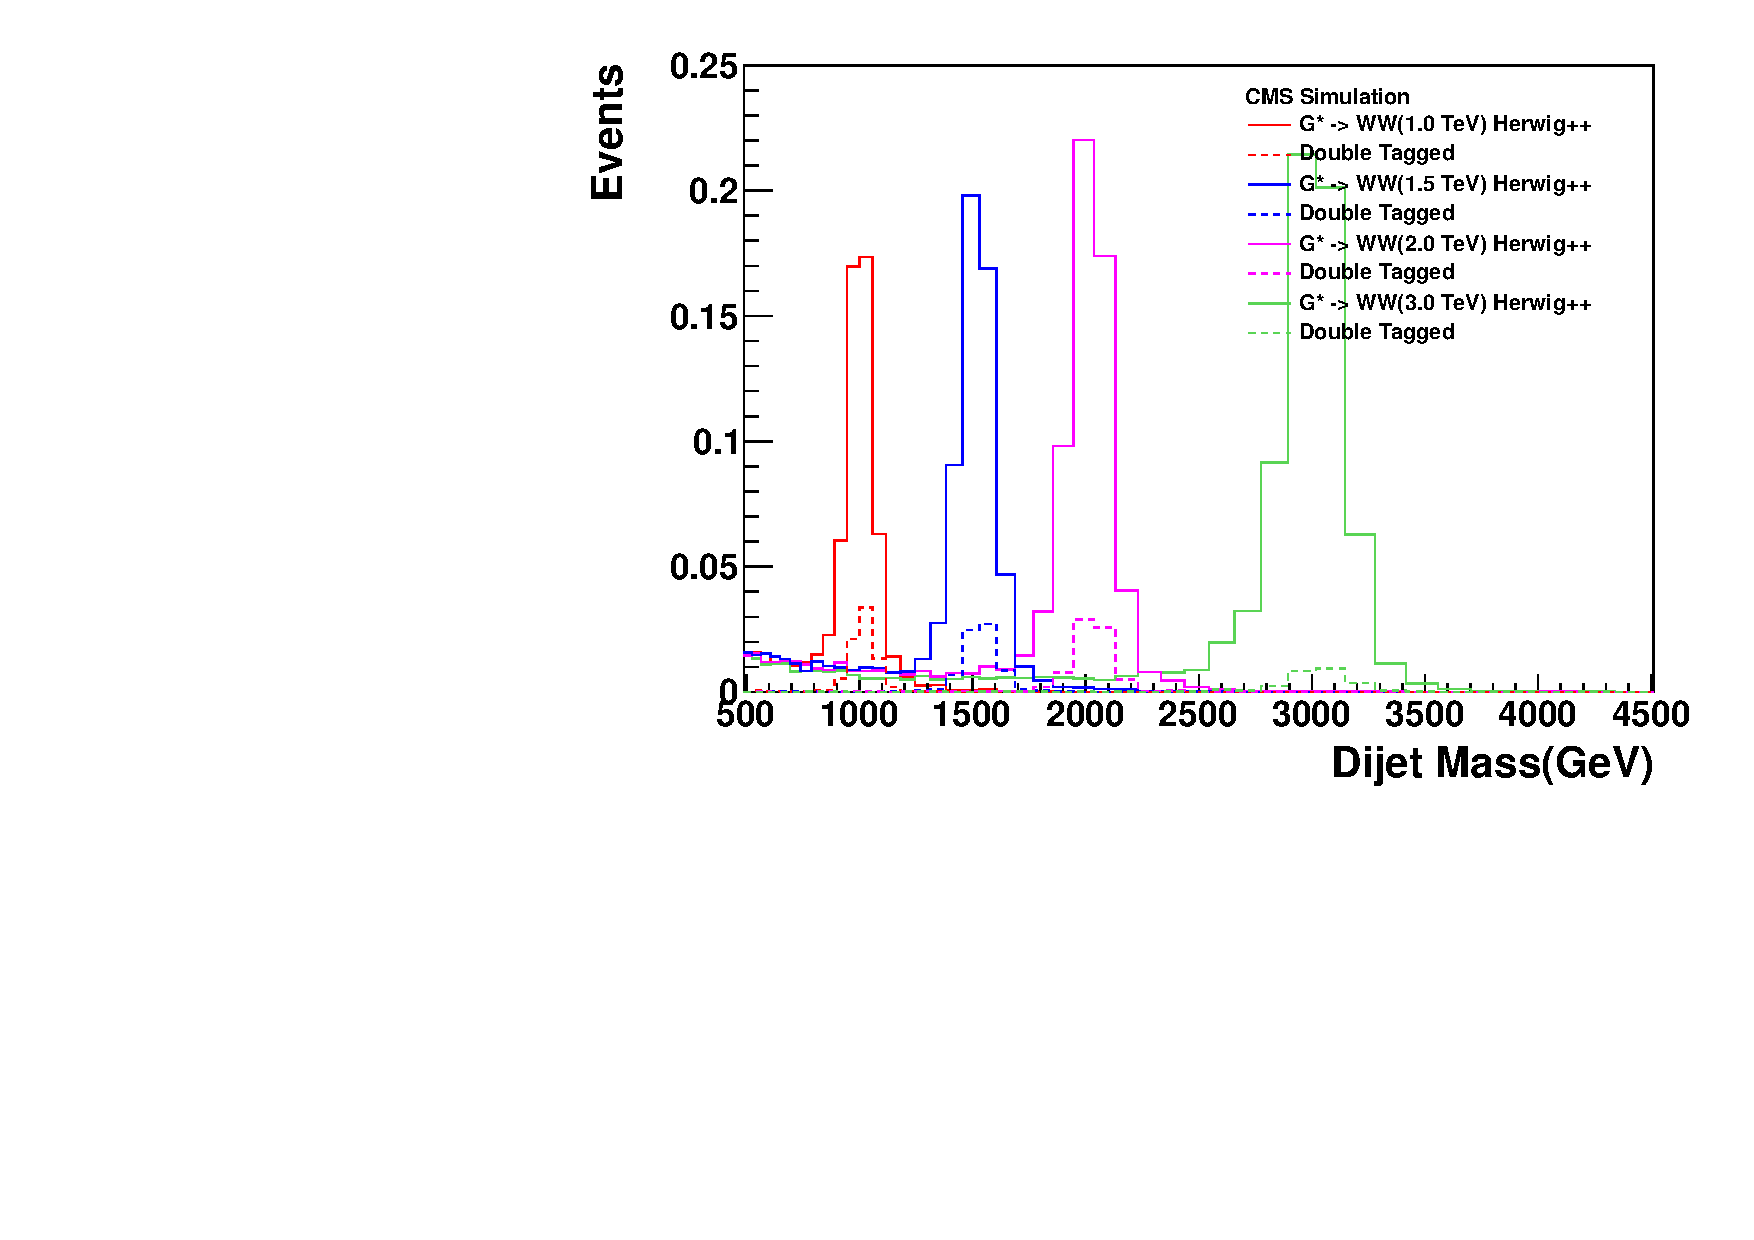
\includegraphics[width=0.48\textwidth]{figs/signal-acc-eff/GstarWWherwig.pdf}
%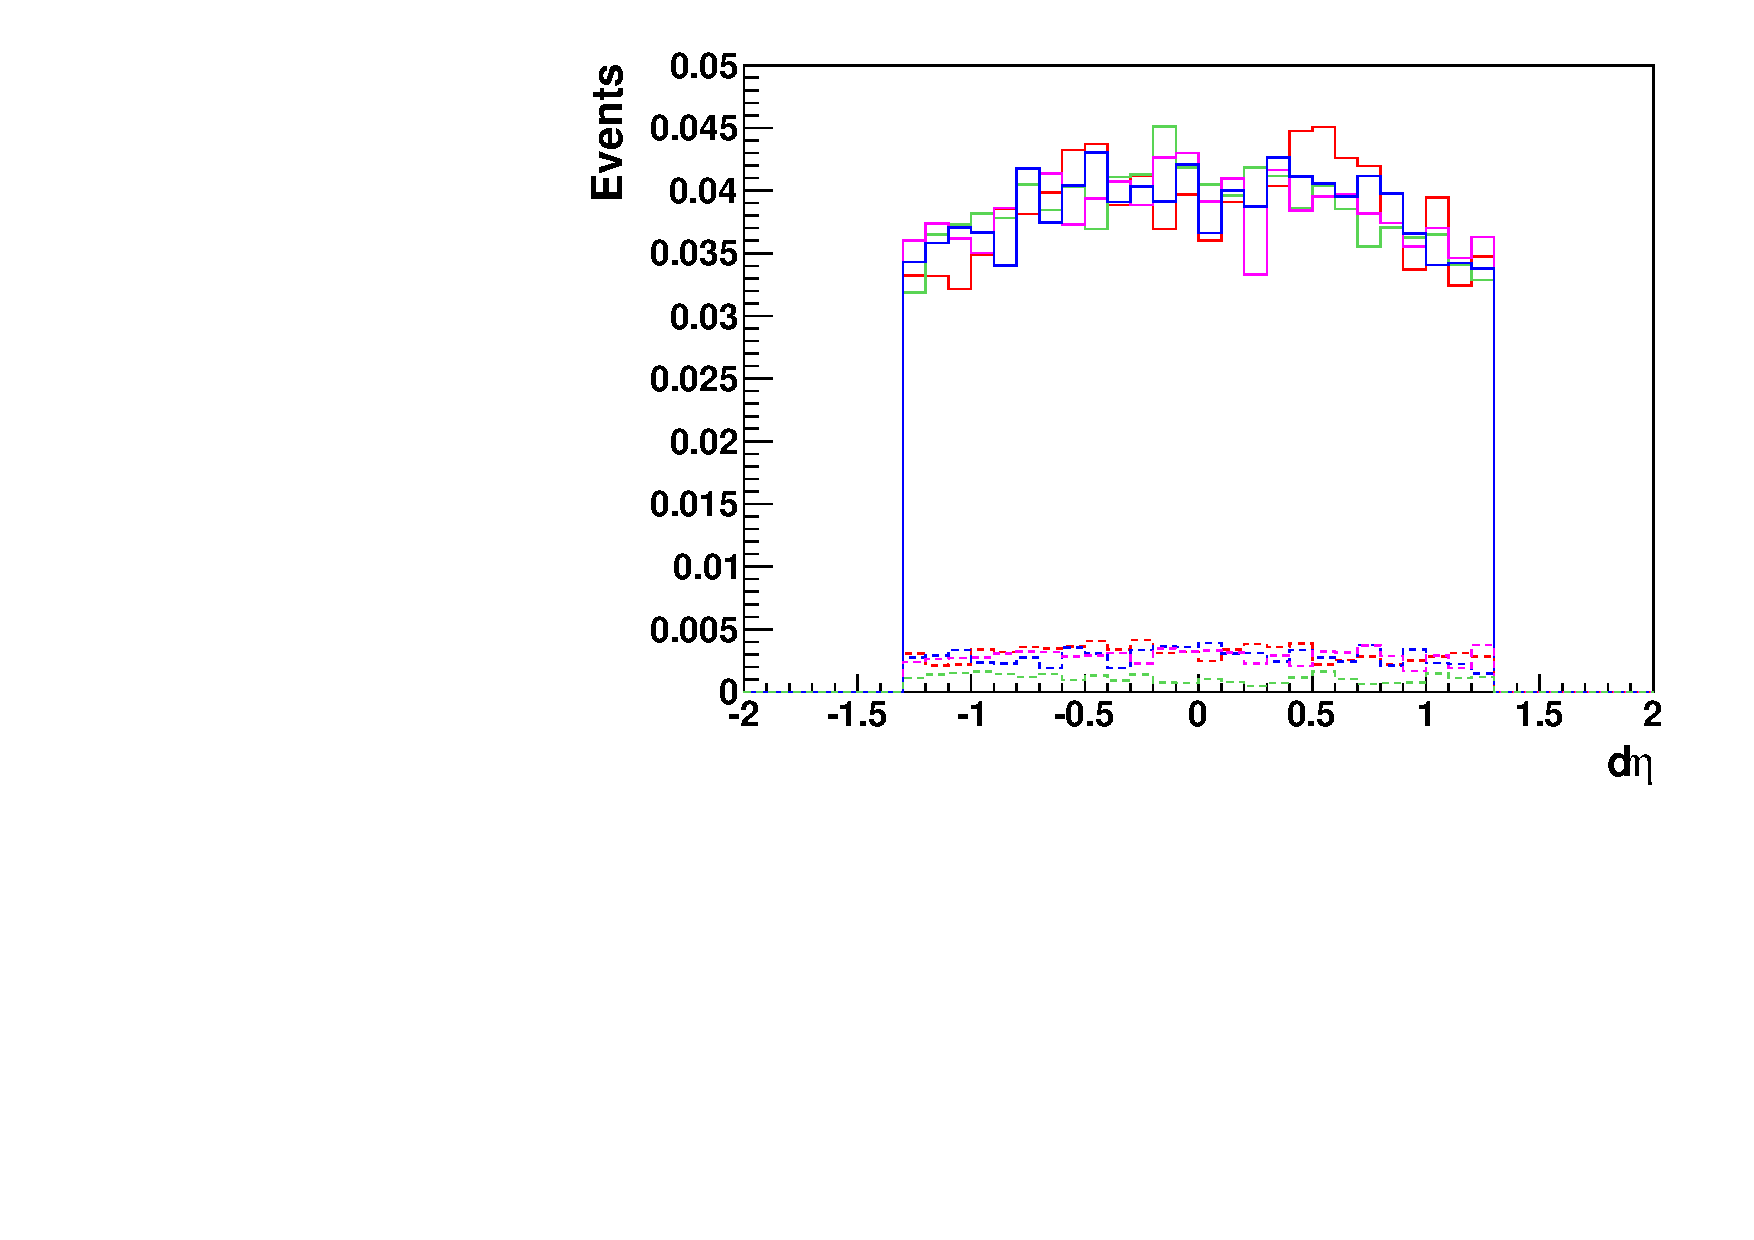
\includegraphics[width=0.48\textwidth]{figs/signal-acc-eff/RSGWWherwig-deta.pdf}
%\end{center}
%\caption{Signal shape in AK5 dijet mass and $\Delta \eta$: $G_{RS} \to WW$ using Herwig++.
%The shape in AK5 dijet mass is normalized to the number of generated events (with phasespace cuts).
%The distribution in $\Delta \eta$ is normalized to the number of events passing the analysis selection in the inclusive category (no W/Z-tagging required).} 
%\label{fig:acceptanceGstarWWherwig}
%\end{figure}


%\begin{figure}[htb]
%\begin{center}
%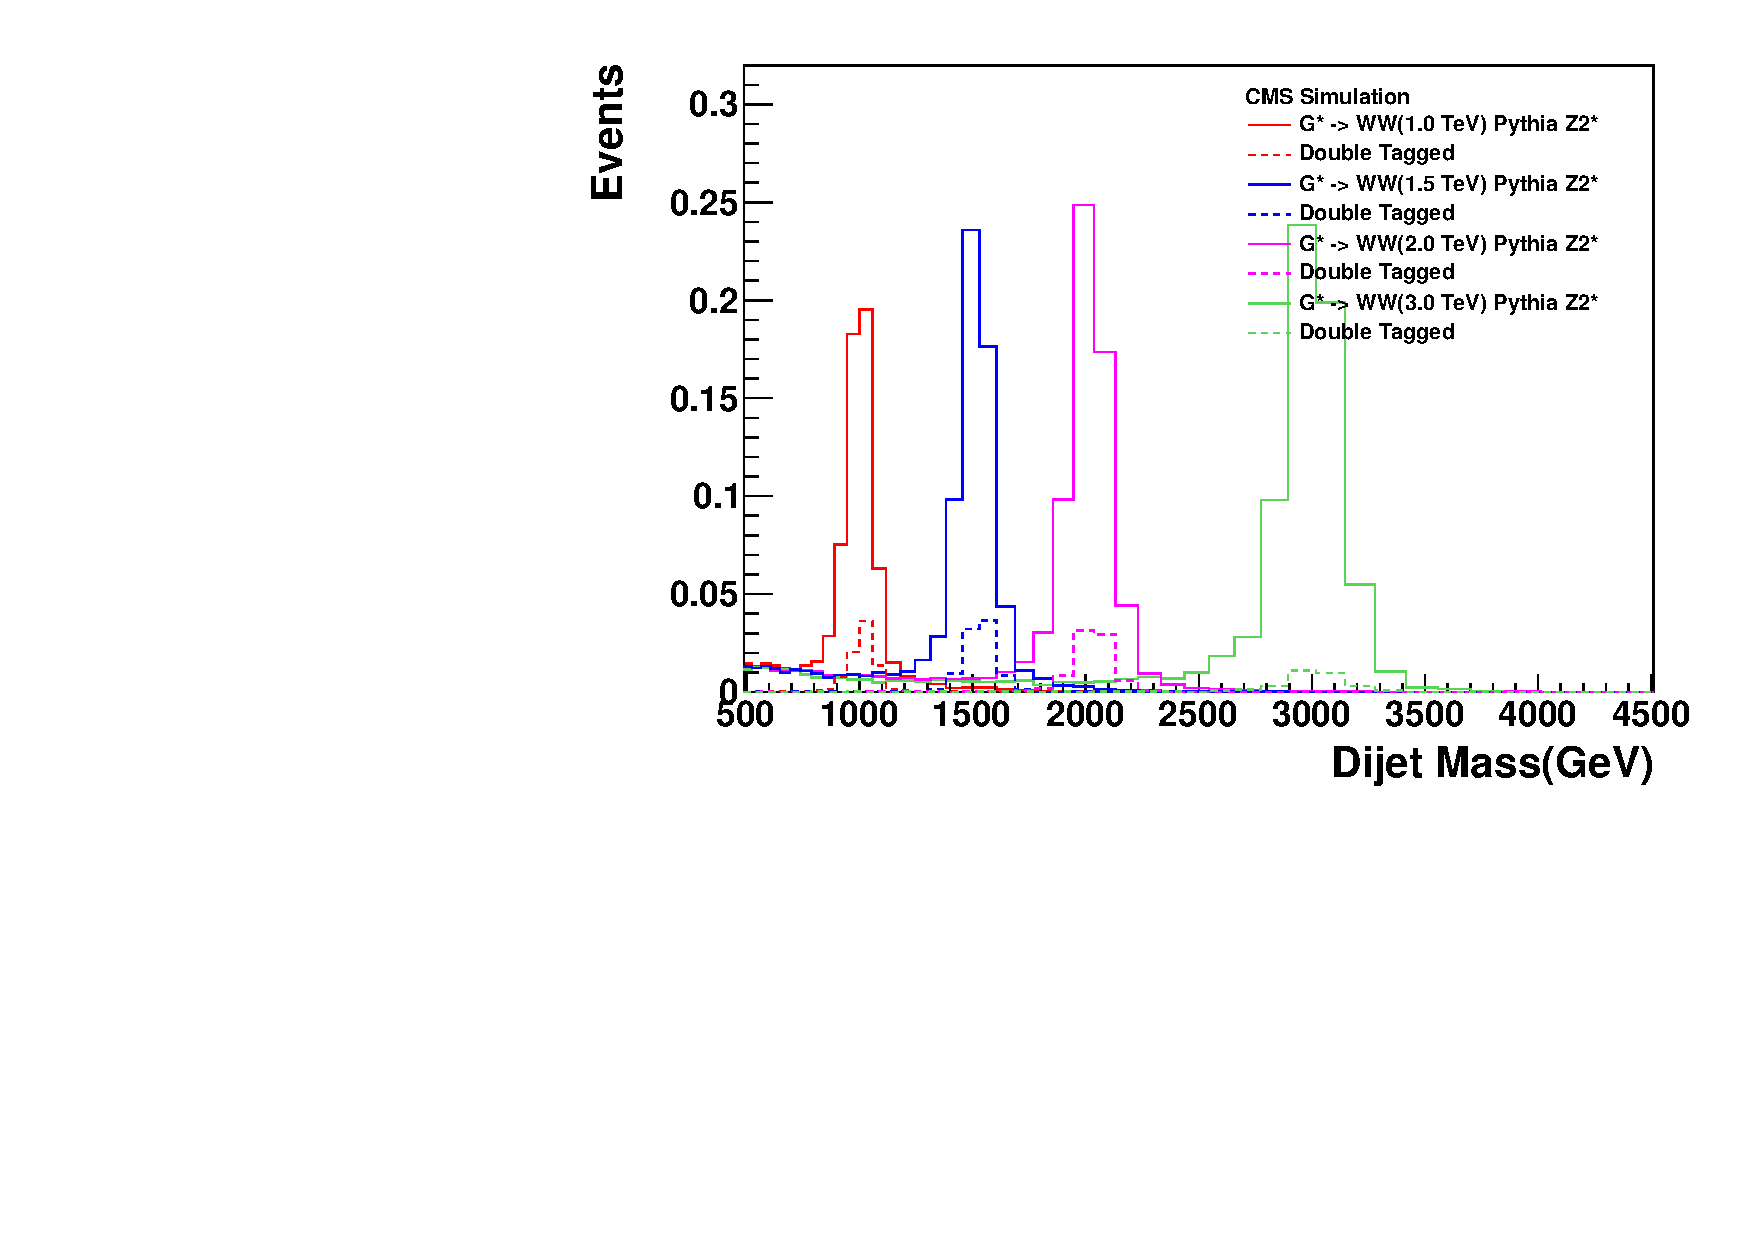
\includegraphics[width=0.48\textwidth]{figs/signal-acc-eff/GstarWWpythia.pdf}
%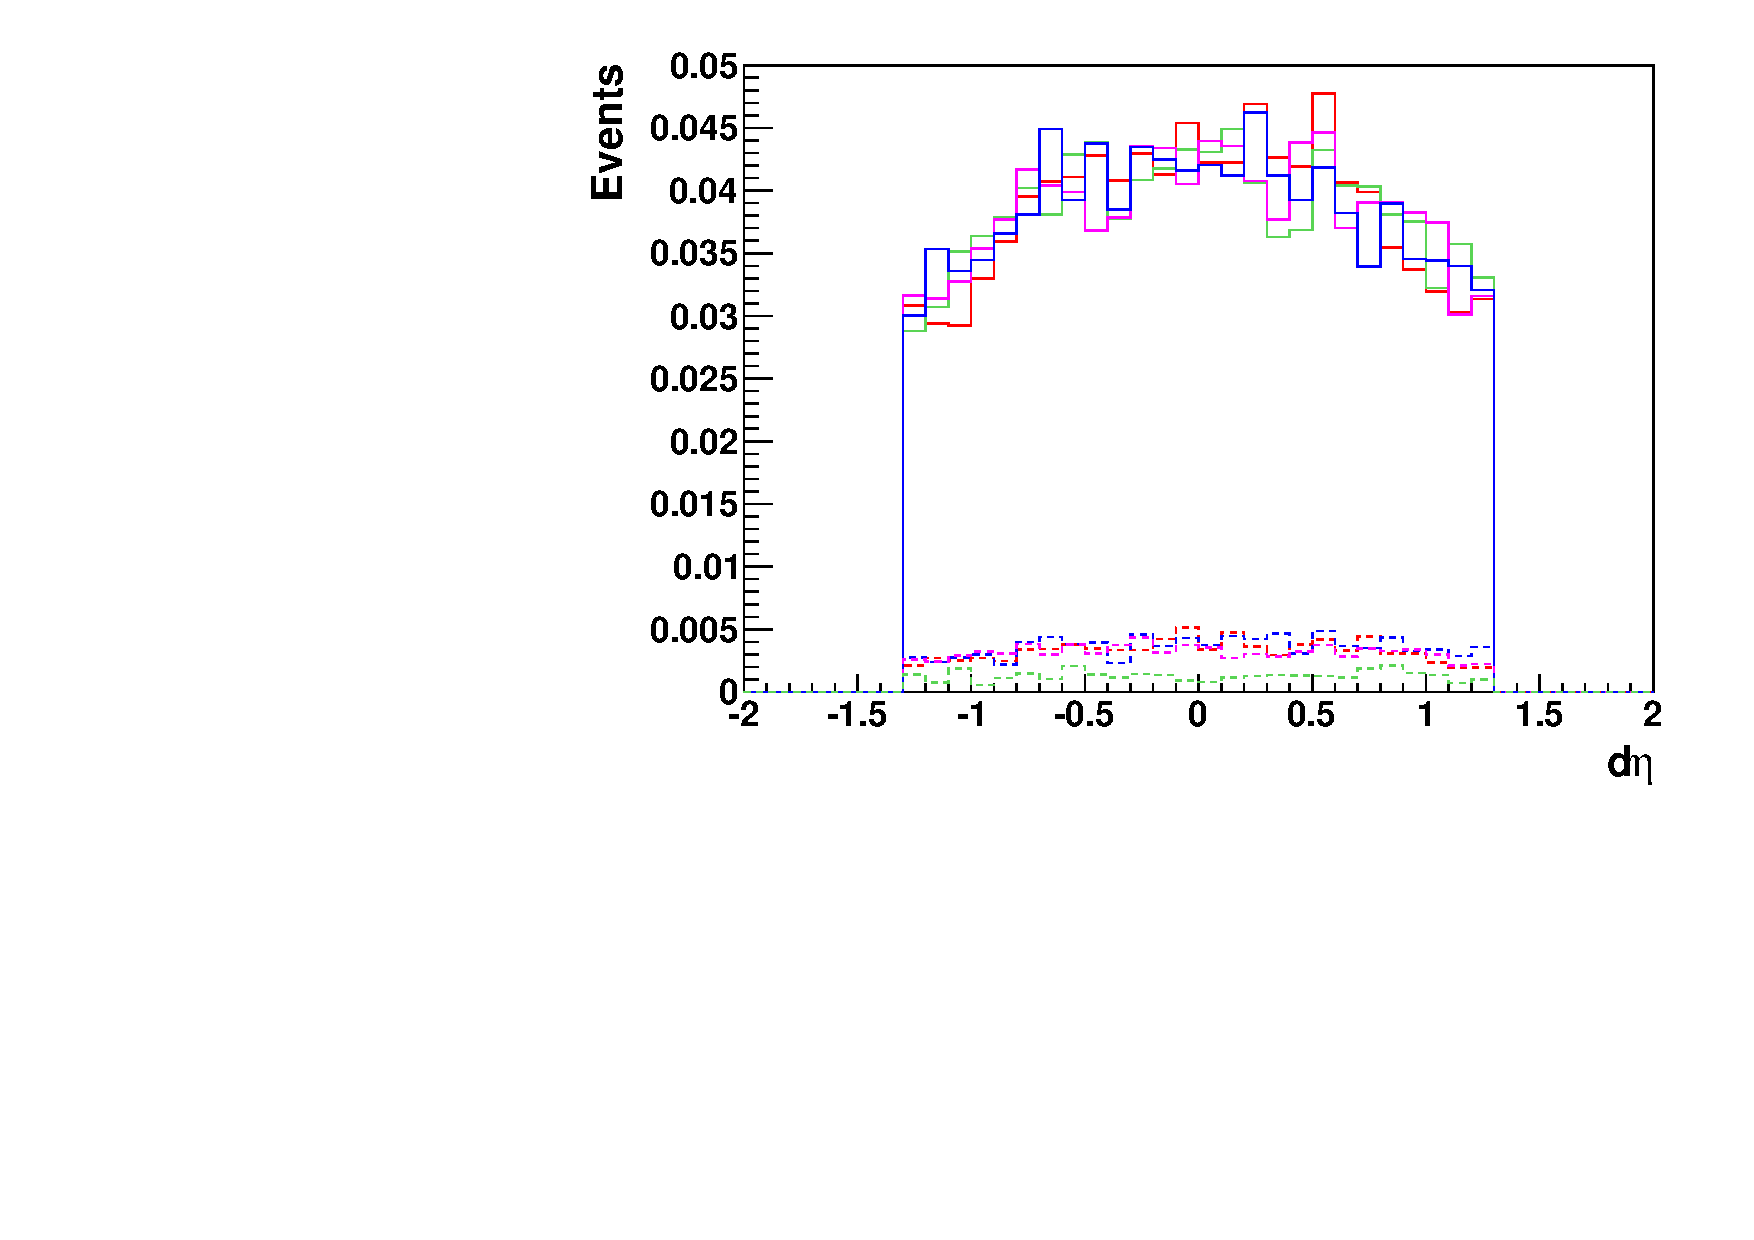
\includegraphics[width=0.48\textwidth]{figs/signal-acc-eff/RSGWWpythia-deta.pdf}
%\end{center}
%\caption{Signal shape in AK5 dijet mass and $\Delta \eta$: $G_{RS} \to WW$ using Pythia Z2*.
%The shape in AK5 dijet mass is normalized to the number of generated events (with phasespace cuts).
%The distribution in $\Delta \eta$ is normalized to the number of events passing the analysis selection in the inclusive category (no W/Z-tagging required).}
%\label{fig:acceptanceGstarWWpythia}
%\end{figure}

%\begin{figure}[htb]
%\begin{center}
%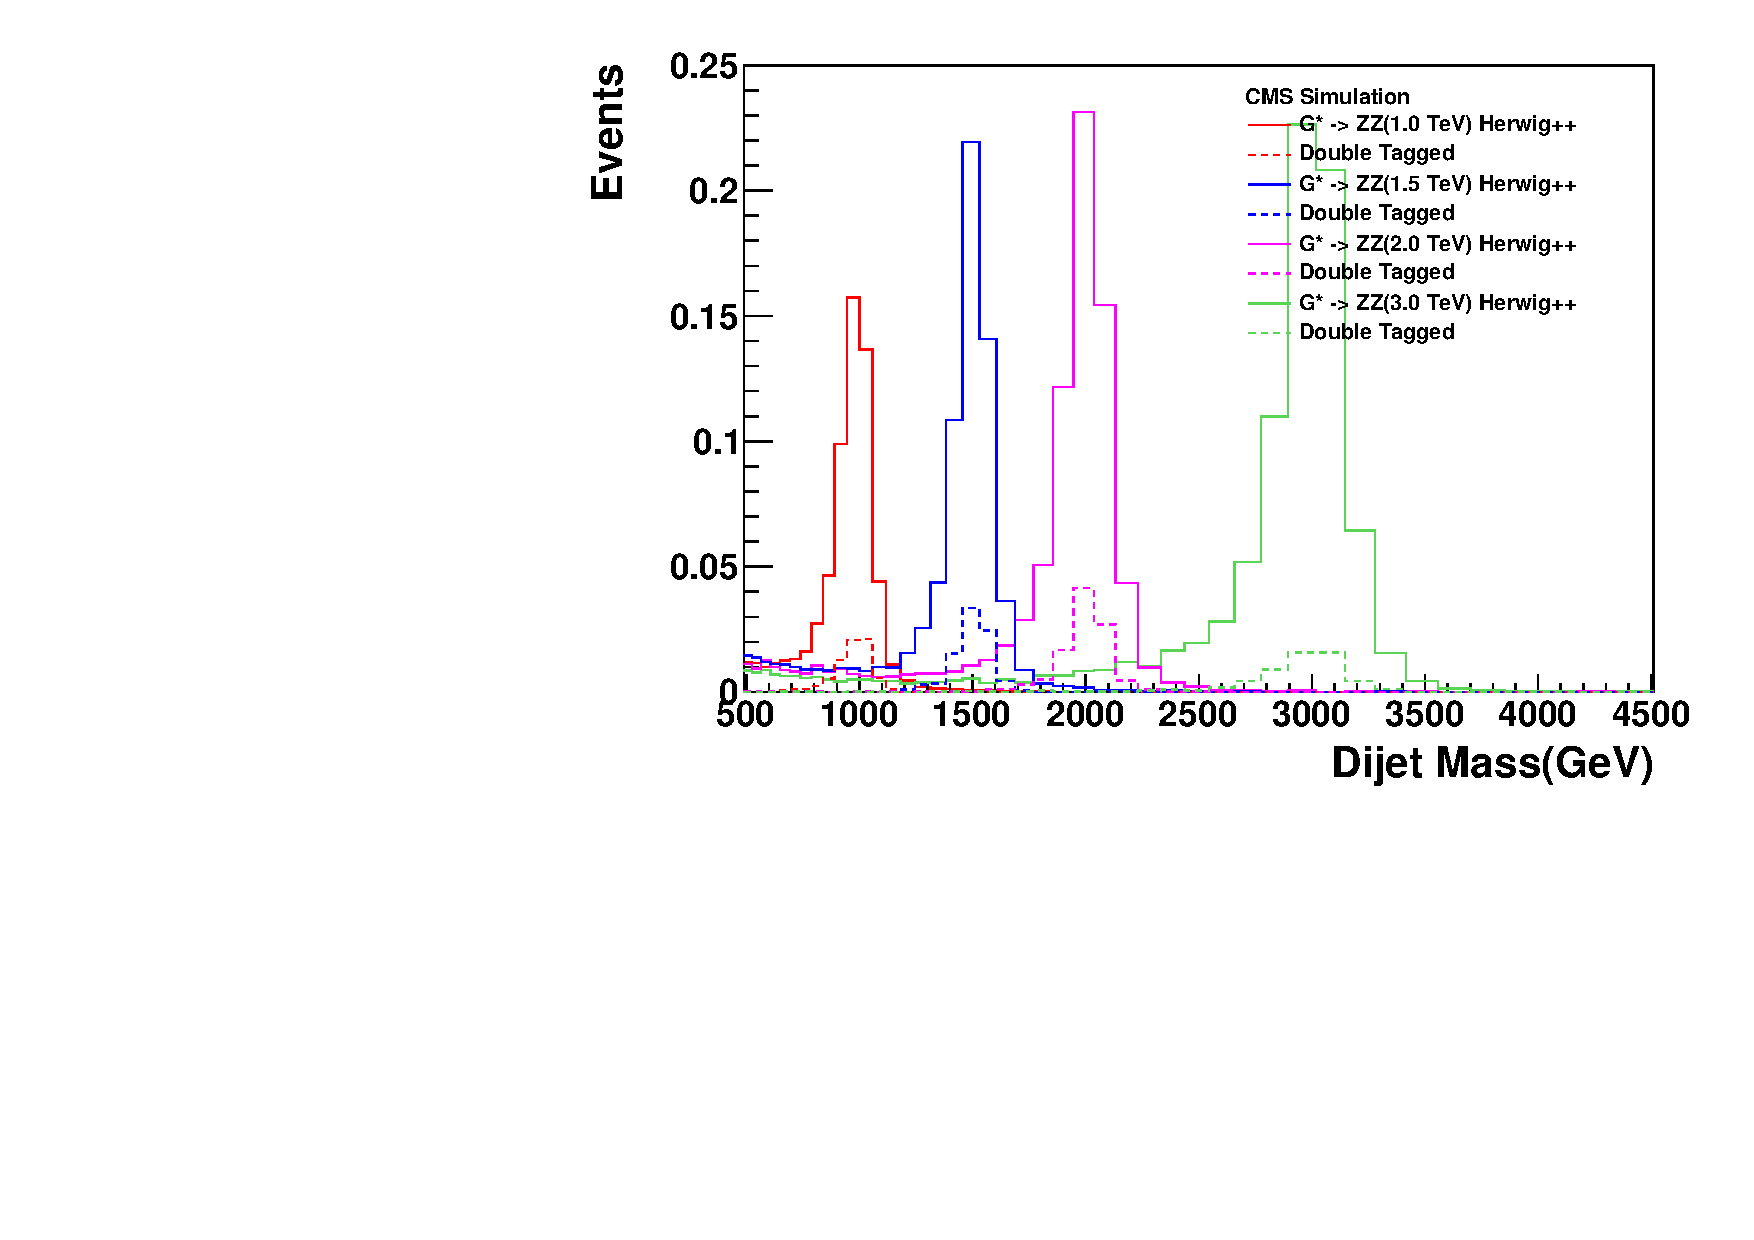
\includegraphics[width=0.48\textwidth]{figs/signal-acc-eff/GstarZZherwig.pdf}
%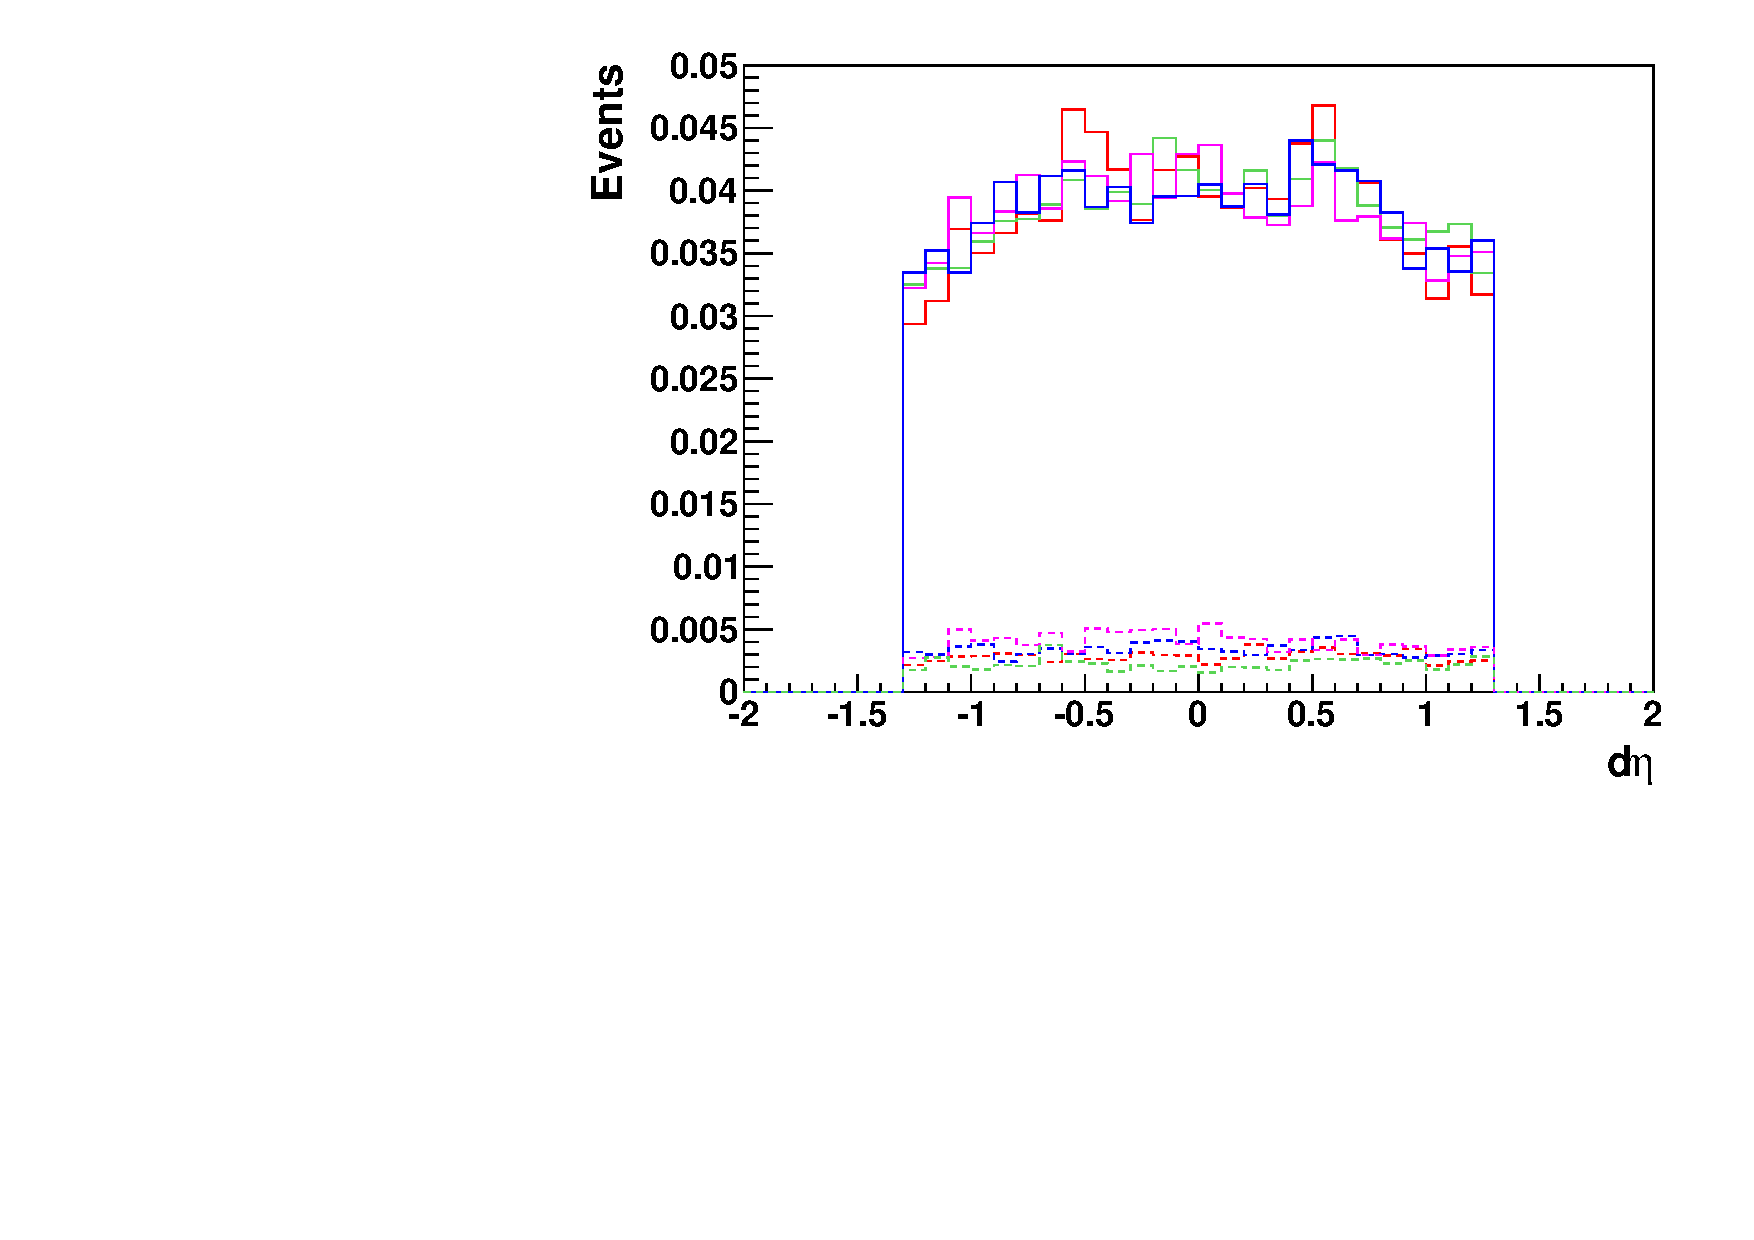
\includegraphics[width=0.48\textwidth]{figs/signal-acc-eff/RSGZZherwig-deta.pdf}
%\end{center}
%\caption{Signal shape in AK5 dijet mass and $\Delta \eta$: $G_{RS} \to ZZ$ using Herwig++.
%The shape in AK5 dijet mass is normalized to the number of generated events (with phasespace cuts).
%The distribution in $\Delta \eta$ is normalized to the number of events passing the analysis selection in the inclusive category (no W/Z-tagging required).}
%\label{fig:acceptanceGstarZZherwig}
%\end{figure}



%\begin{figure}[htb]
%\begin{center}
%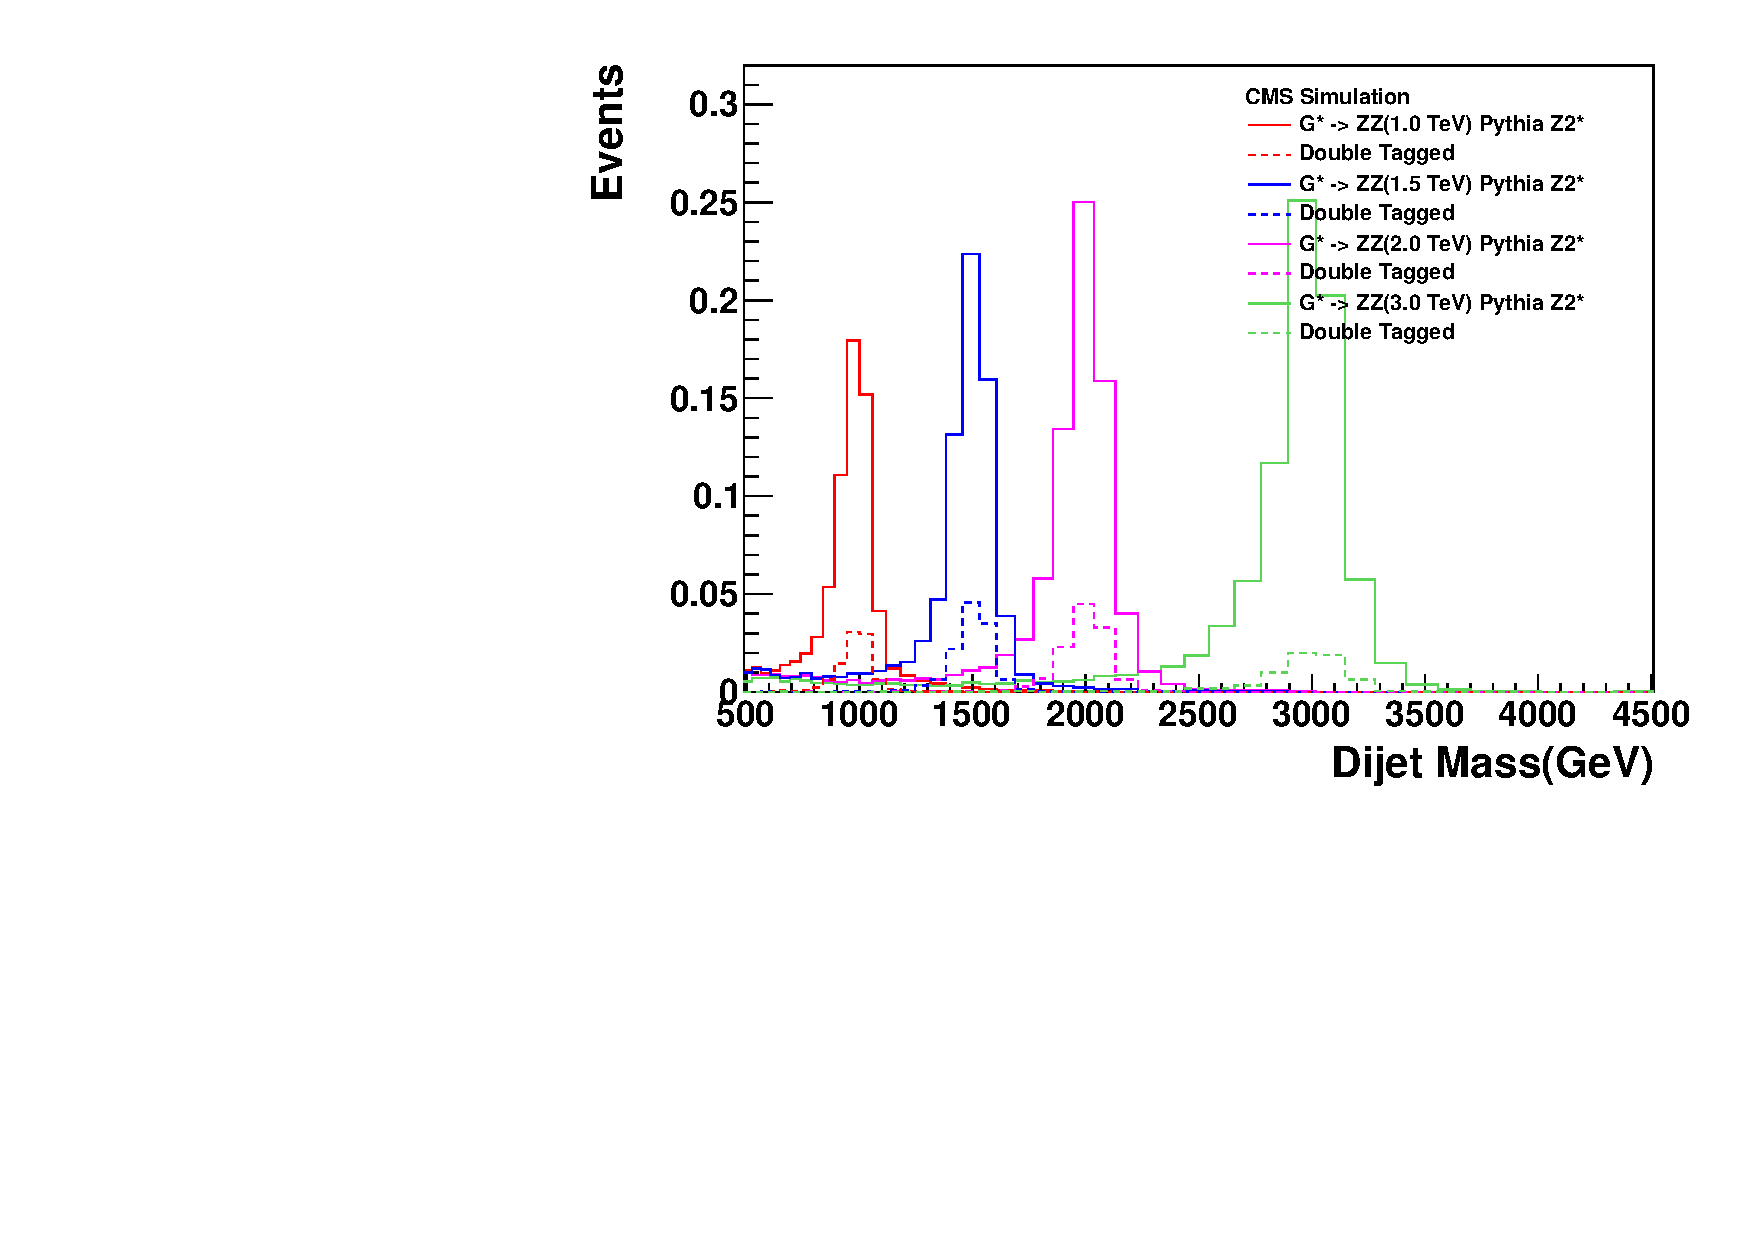
\includegraphics[width=0.48\textwidth]{figs/signal-acc-eff/GstarZZpythia.pdf}
%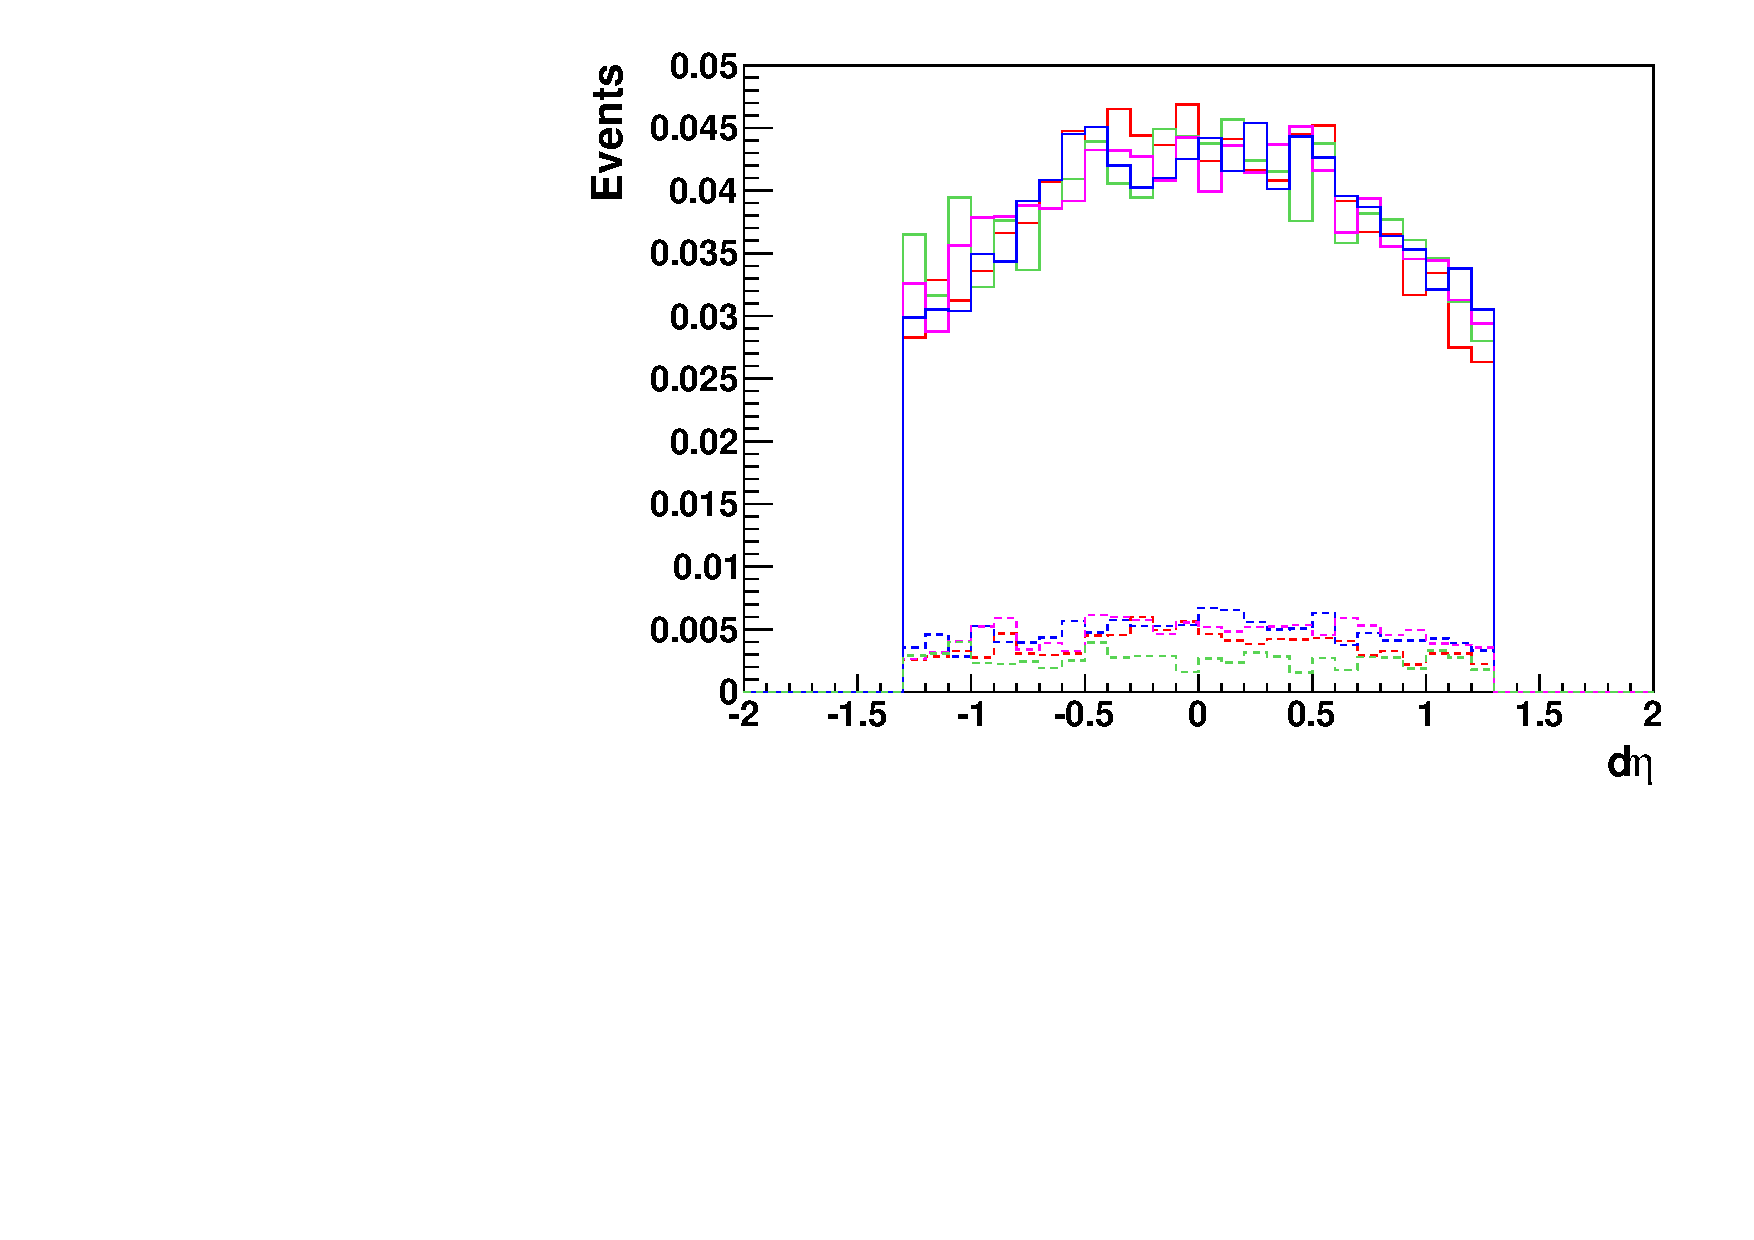
\includegraphics[width=0.48\textwidth]{figs/signal-acc-eff/RSGZZpythia-deta.pdf}
%\end{center}
%\caption{Signal shape in AK5 dijet mass and $\Delta \eta$: $G_{RS} \to ZZ$ using Pythia Z2*.
%The shape in AK5 dijet mass is normalized to the number of generated events (with phasespace cuts).
%The distribution in $\Delta \eta$ is normalized to the number of events passing the analysis selection in the inclusive category (no W/Z-tagging required).}
%\label{fig:acceptanceGstarZZpythia}
%\end{figure}


%\begin{figure}[htb]
%\begin{center}
%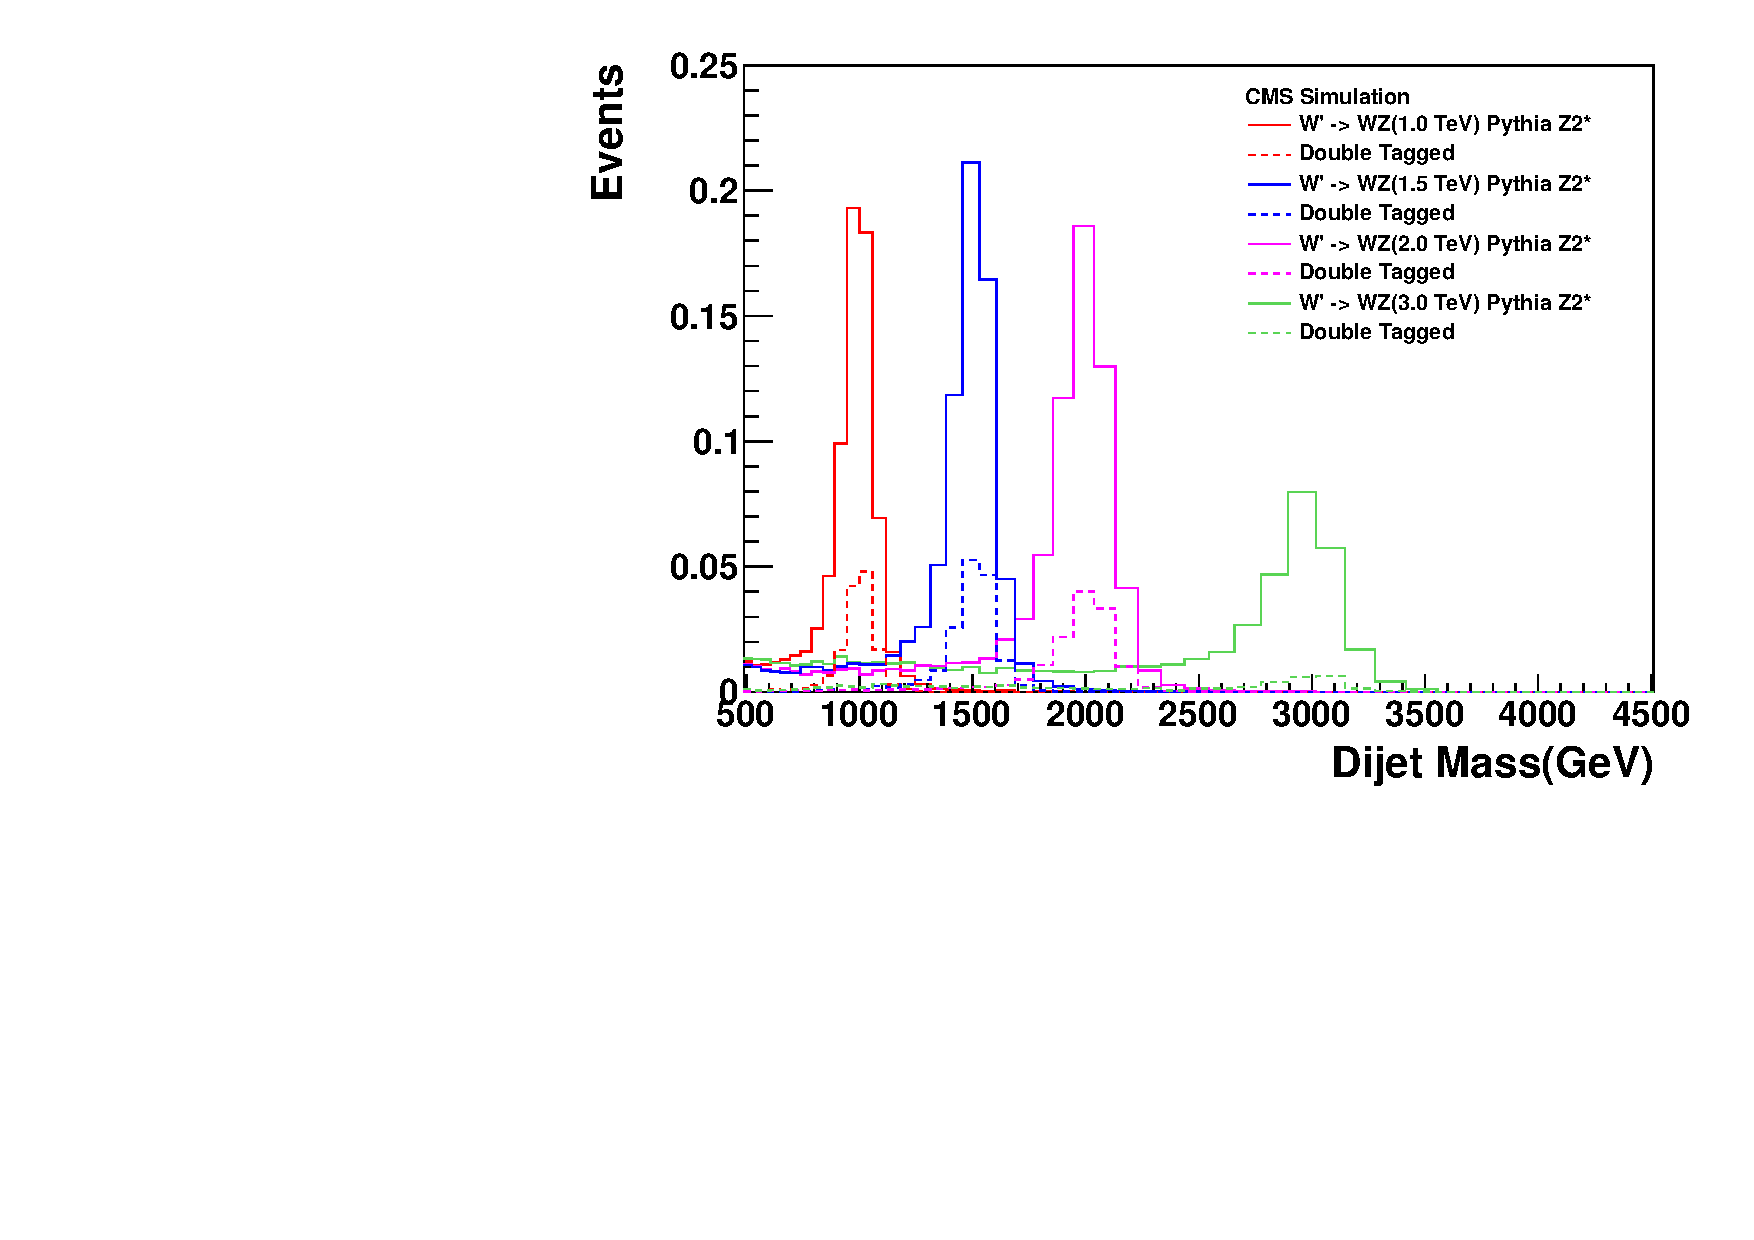
\includegraphics[width=0.48\textwidth]{figs/signal-acc-eff/WZWprime.pdf}
%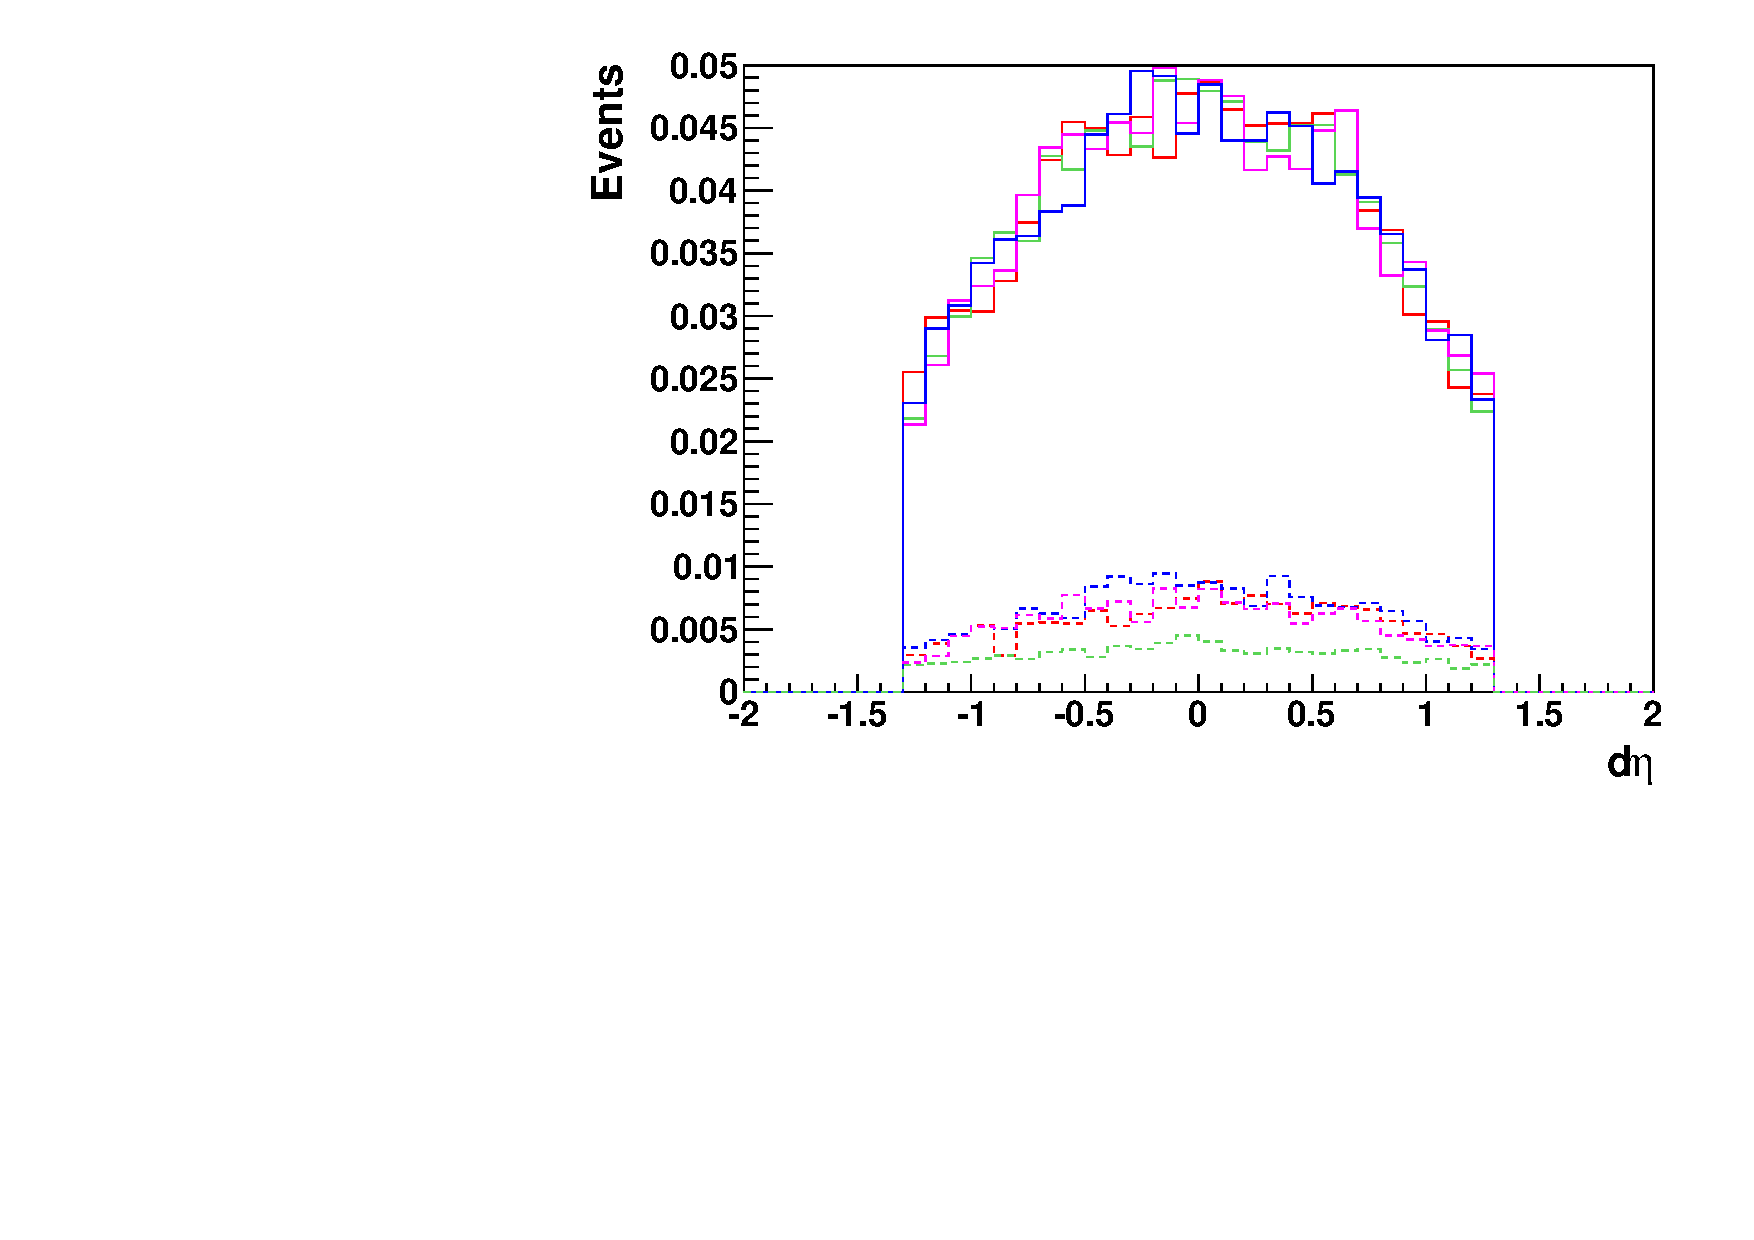
\includegraphics[width=0.48\textwidth]{figs/signal-acc-eff/Wprime-deta.pdf}
%\end{center}
%\caption{Signal shape in AK5 dijet mass and $\Delta \eta$: $W' \to WZ$.
%The shape in AK5 dijet mass is normalized to the number of generated events (with phasespace cuts).
%The distribution in $\Delta \eta$ is normalized to the number of events passing the analysis selection in the inclusive category (no W/Z-tagging required).}
%\label{fig:acceptanceWprime}
%\end{figure}

%\begin{figure}[htb]
%\begin{center}
%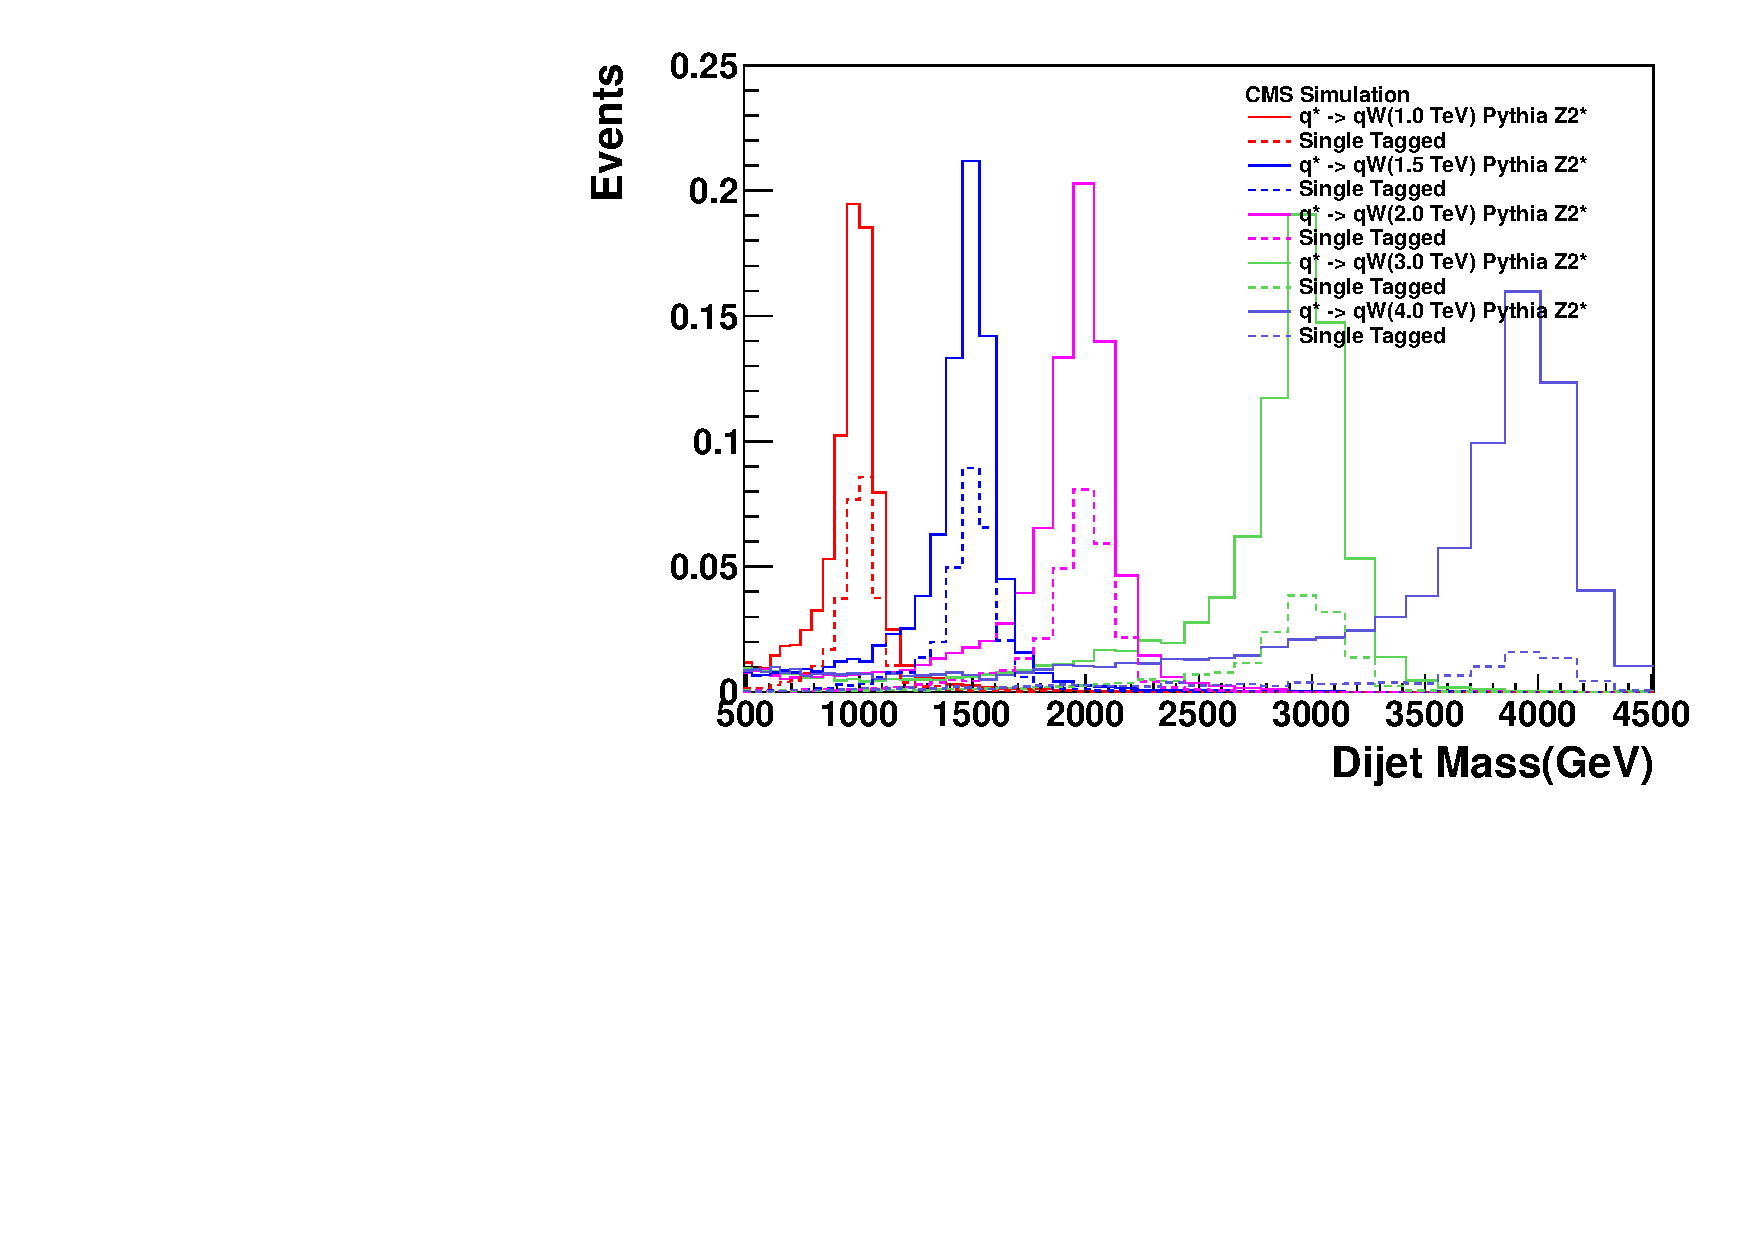
\includegraphics[width=0.48\textwidth]{figs/signal-acc-eff/qstarqw.pdf}
%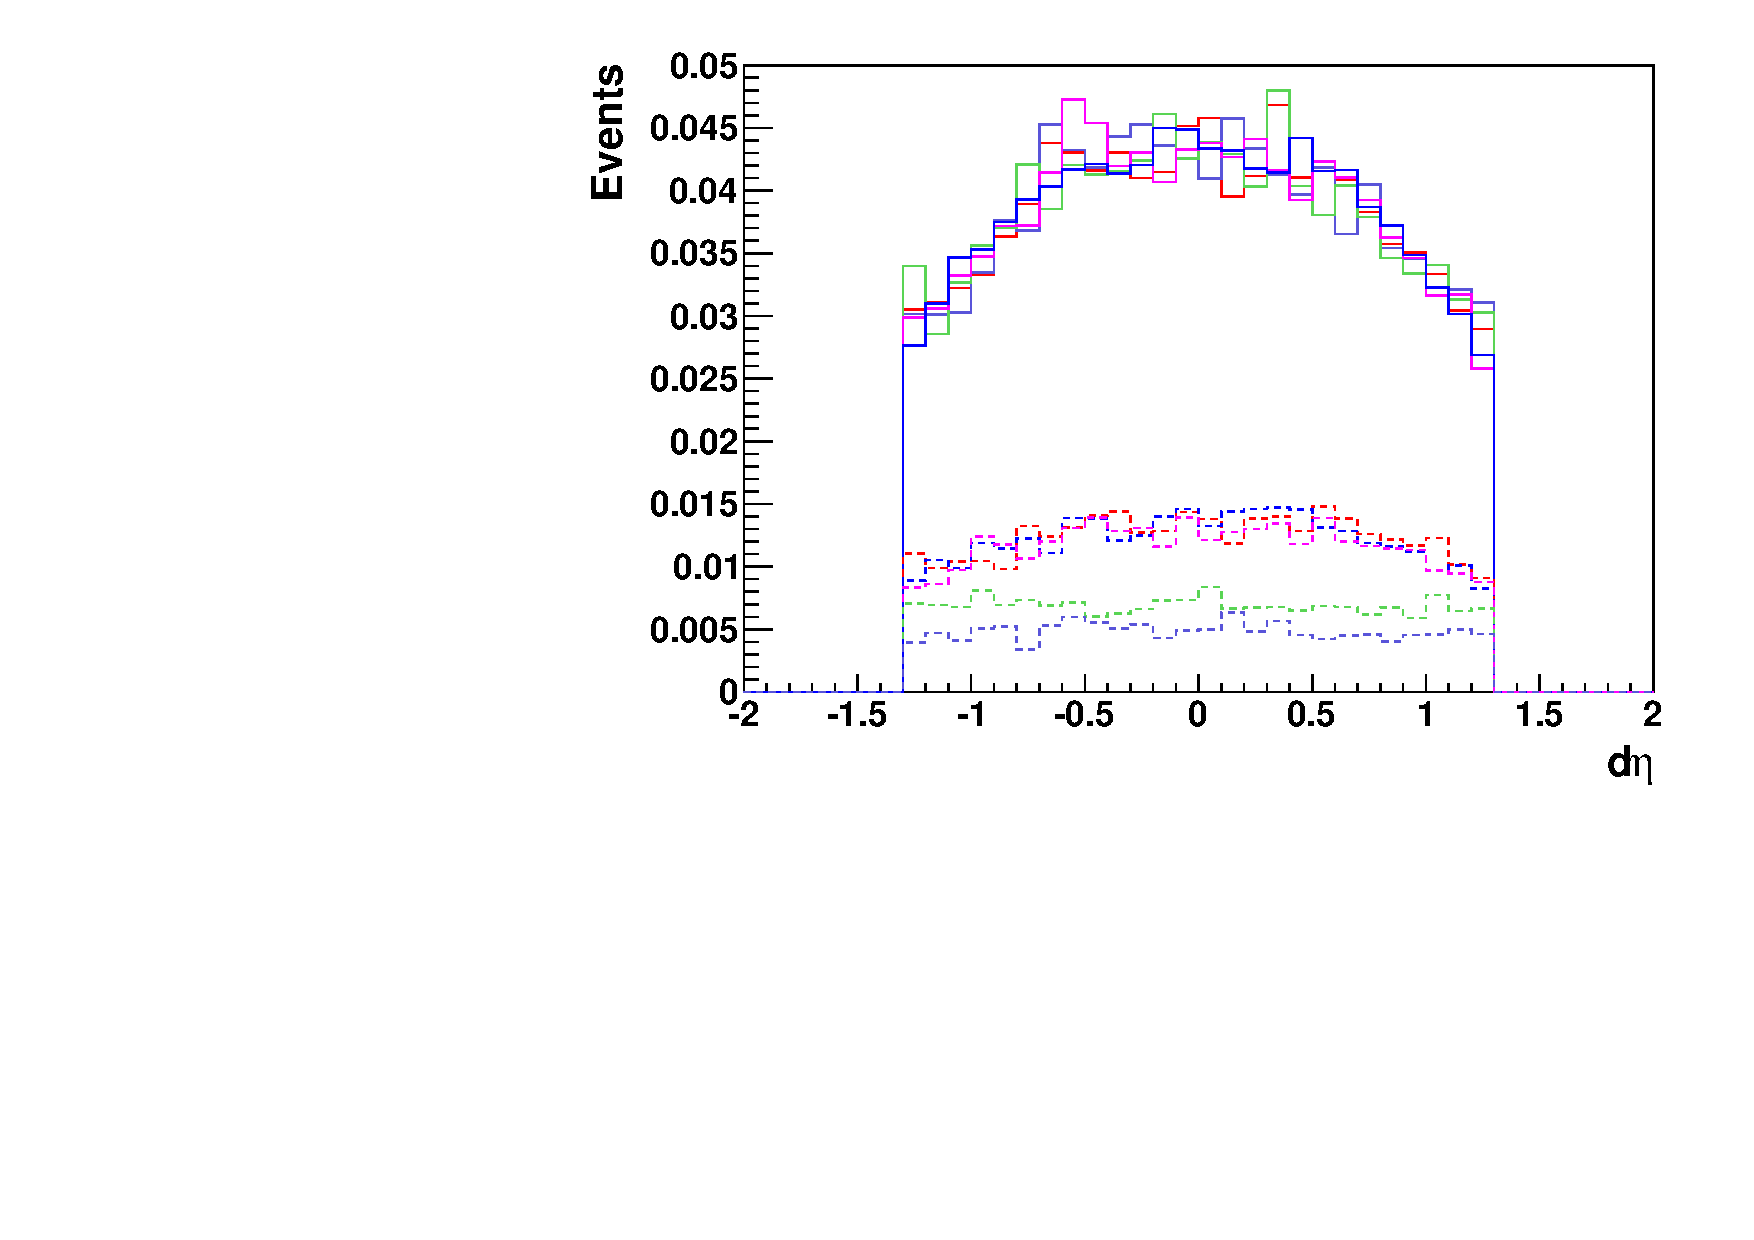
\includegraphics[width=0.48\textwidth]{figs/signal-acc-eff/QstarToQW-deta.pdf}
%\end{center}
%\caption{Signal shape in AK5 dijet mass and $\Delta \eta$: $q*\to qW$.
%The shape in AK5 dijet mass is normalized to the number of generated events (with phasespace cuts).
%The distribution in $\Delta \eta$ is normalized to the number of events passing the analysis selection in the inclusive category (no W/Z-tagging required).}
%\label{fig:acceptanceqstarqW}
%\end{figure}

%\begin{figure}[htb]
%\begin{center}
%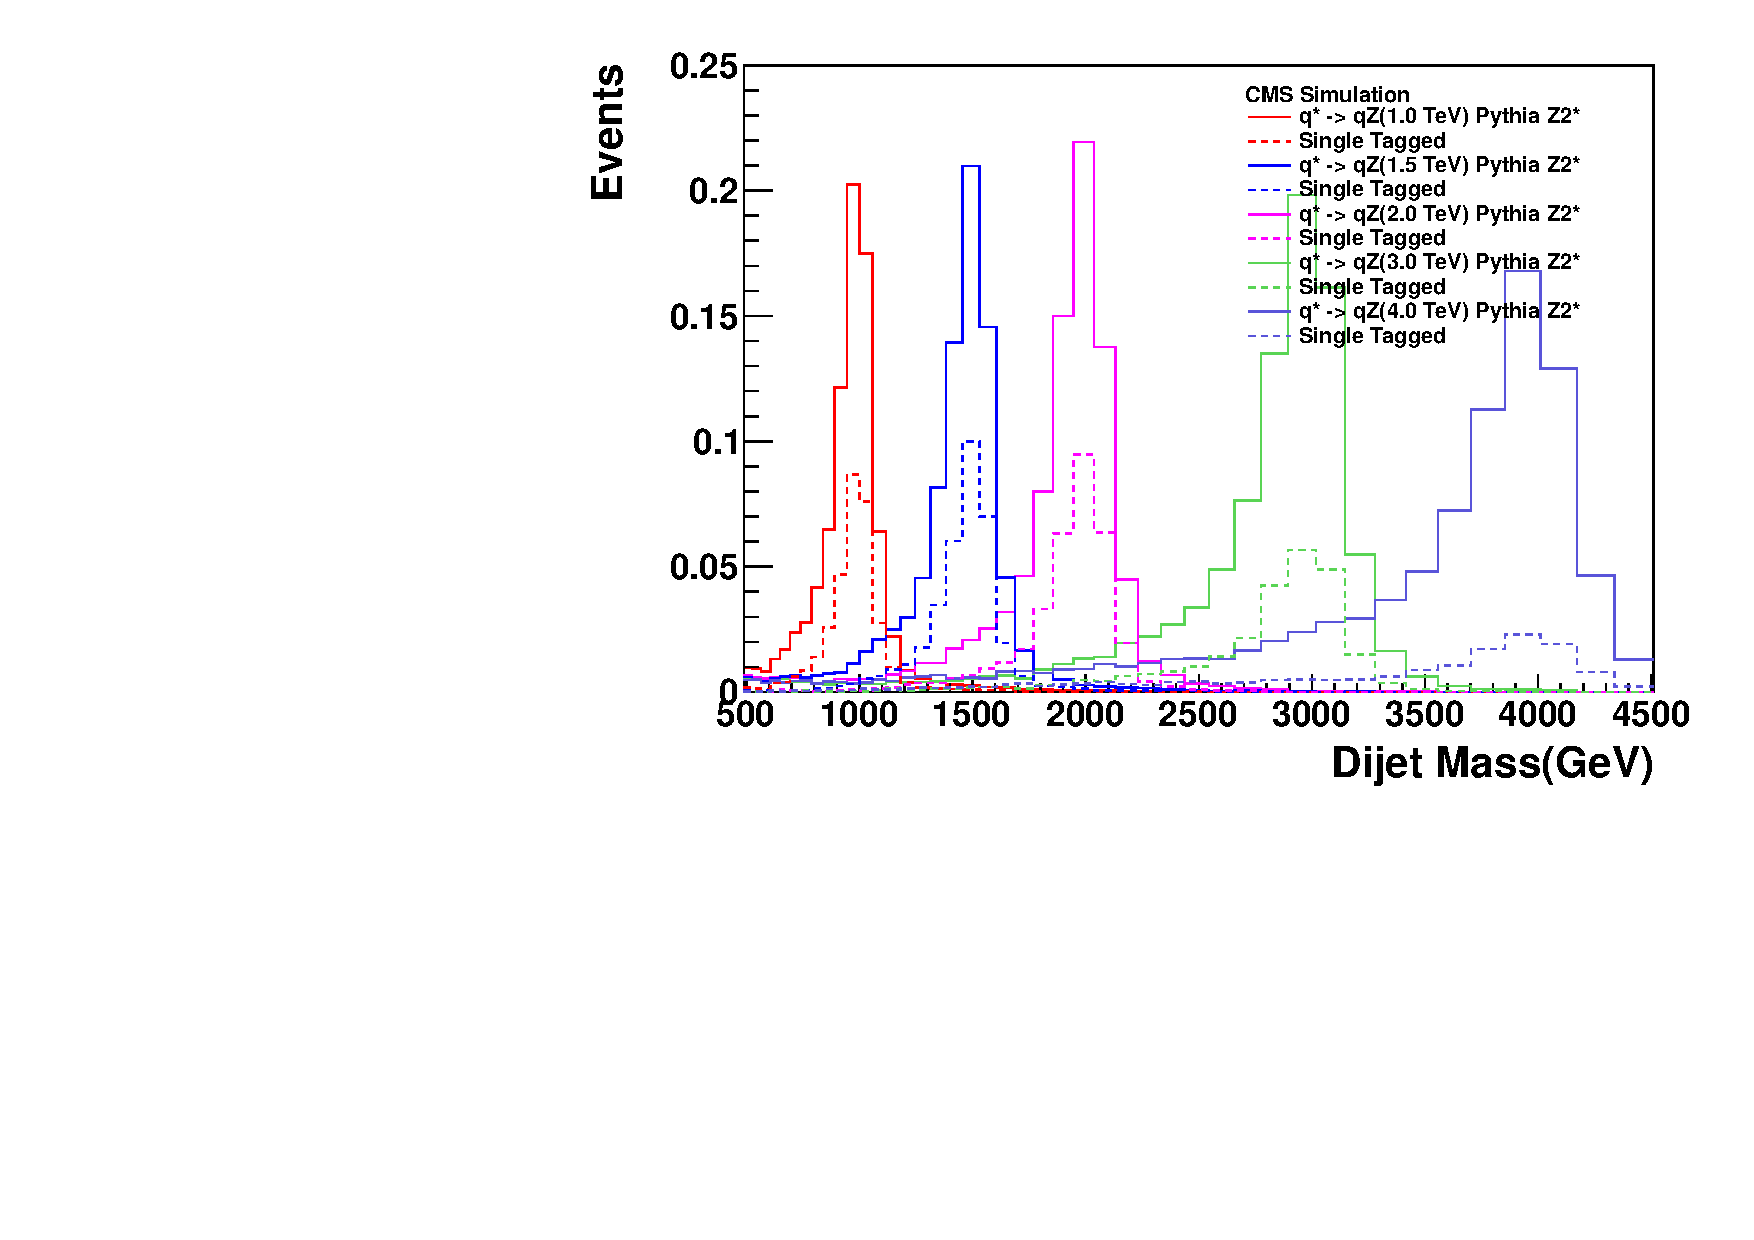
\includegraphics[width=0.48\textwidth]{figs/signal-acc-eff/qstarqz.pdf}
%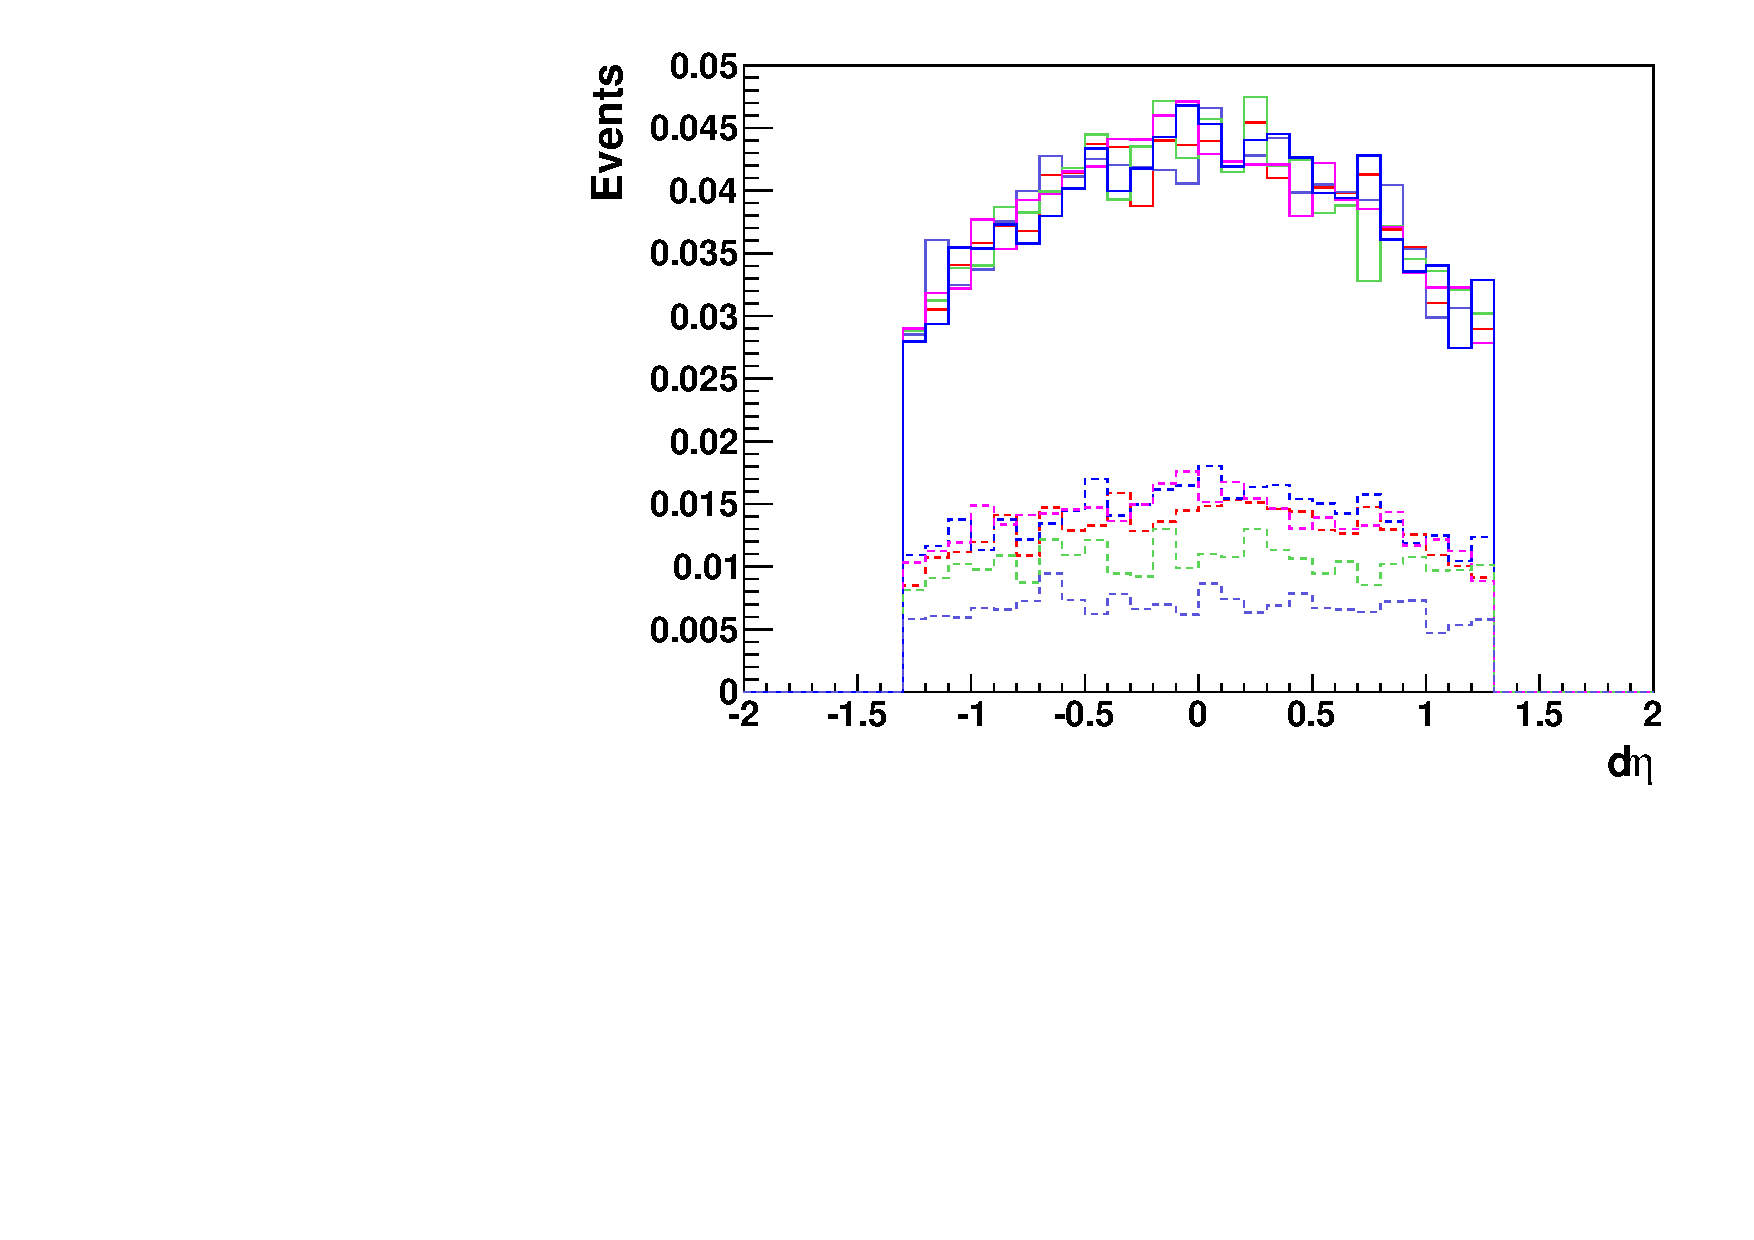
\includegraphics[width=0.48\textwidth]{figs/signal-acc-eff/QstarToQZ-deta.pdf}
%\end{center}
%\caption{Signal shape in AK5 dijet mass and $\Delta \eta$: $q*\to qZ$.
%The shape in AK5 dijet mass is normalized to the number of generated events (with phasespace cuts).
%The distribution in $\Delta \eta$ is normalized to the number of events passing the analysis selection in the inclusive category (no W/Z-tagging required).}
%\label{fig:acceptanceqstarqZ}
%\end{figure}
\fi

{\bf we will add the signal shapes here. and the overall signal tagging efficiency and data tagging efficiency.  }


\clearpage

